%\pdfoutput=1
% Uncomment line above if submitting to arXiv and using pdflatex

% $Id: main.tex 33041 2013-03-25 16:12:53Z tgershon $
% ============================================================================
% Purpose: Template for LHCb documents
% Authors: Tomasz Skwarnicki, Roger Forty, Ulrik Egede
% Modified by: Adam Elwood
% Created on: 2010-09-24
% ============================================================================
\documentclass[12pt,a4paper]{article}
% For two column text, add "twocolumn" as an option to the document
% class. Also uncomment the two "onecolumn" and "twocolumn" lines
% around the title page below.

% Variables that controls behaviour
\usepackage{ifthen} % for conditional statements
\newboolean{pdflatex}
\setboolean{pdflatex}{true} % False for eps figures 

\newboolean{articletitles}
\setboolean{articletitles}{true} % False removes titles in references

\newboolean{uprightparticles}
\setboolean{uprightparticles}{false} %True for upright particle symbols

%\newboolean{inbibliography}
%\setboolean{inbibliography}{false} %True once you enter the bibliography

% THis file contains all the default packages and modifications for
% LHCb formatting

%% %%%%%%%%%%%%%%%%%%
%%  Page formatting
%% %%%%%%%%%%%%%%%%%%
\textheight=230mm
\textwidth=160mm
\oddsidemargin=7mm
\evensidemargin=-10mm
\topmargin=-10mm
\headsep=20mm
\columnsep=5mm
\addtolength{\belowcaptionskip}{0.5em}

\renewcommand{\textfraction}{0.01}
\renewcommand{\floatpagefraction}{0.99}
\renewcommand{\topfraction}{0.9}
\renewcommand{\bottomfraction}{0.9}


\setlength{\hoffset}{-2cm}
\setlength{\voffset}{-2cm}
% Page defaults ...
\topmargin=0.5cm
\oddsidemargin=2.5cm
\textwidth=16cm
\textheight=22cm
% Allow the page size to vary a bit ...
\raggedbottom
% To avoid Latex to be too fussy with line breaking ...
%\sloppy

%% %%%%%%%%%%%%%%%%%%%%%%%
%% Packages to be used
%% %%%%%%%%%%%%%%%%%%%%%%% 
\usepackage{microtype}
\usepackage{lineno}  % for line numbering during review
\usepackage{xspace} % To avoid problems with missing or double spaces after
                    % predefined symbold
\usepackage{caption} %these three command get the figure and table captions automatically small
\renewcommand{\captionfont}{\small}
\renewcommand{\captionlabelfont}{\small}

%% Graphics
\usepackage{graphicx}  % to include figures (can also use other packages)
\usepackage{color}
\usepackage{colortbl}
\graphicspath{{./figs/}} % Make Latex search fig subdir for figures
\usepackage{cancel}
\usepackage{subfigure}

%% Math
\usepackage{amsmath} % Adds a large collection of math symbols
\usepackage{amssymb}
\usepackage{amsfonts}
\usepackage{upgreek} % Adds in support for greek letters in roman typeset

%% fix to allow peaceful coexistence of line numbering and
%% mathematical objects
%% http://www.latex-community.org/forum/viewtopic.php?f=5&t=163
%%
\newcommand*\patchAmsMathEnvironmentForLineno[1]{%
\expandafter\let\csname old#1\expandafter\endcsname\csname #1\endcsname
\expandafter\let\csname oldend#1\expandafter\endcsname\csname
end#1\endcsname
 \renewenvironment{#1}%
   {\linenomath\csname old#1\endcsname}%
   {\csname oldend#1\endcsname\endlinenomath}%
}
\newcommand*\patchBothAmsMathEnvironmentsForLineno[1]{%
  \patchAmsMathEnvironmentForLineno{#1}%
  \patchAmsMathEnvironmentForLineno{#1*}%
}
\AtBeginDocument{%
\patchBothAmsMathEnvironmentsForLineno{equation}%
\patchBothAmsMathEnvironmentsForLineno{align}%
\patchBothAmsMathEnvironmentsForLineno{flalign}%
\patchBothAmsMathEnvironmentsForLineno{alignat}%
\patchBothAmsMathEnvironmentsForLineno{gather}%
\patchBothAmsMathEnvironmentsForLineno{multline}%
}

% Get hyperlinks to captions and in references.
% These do not work with revtex. Use "hypertext" as class option instead.
\usepackage{hyperref}    % Hyperlinks in references
\usepackage[all]{hypcap} % Internal hyperlinks to floats.

%%% $Id: lhcb-symbols-def.tex 39235 2013-07-16 11:13:01Z roldeman $
%%% ======================================================================
%%% Purpose: Standard LHCb aliases
%%% Author: Originally Ulrik Egede, adapted by Tomasz Skwarnicki for templates,
%%% rewritten by Chris Parkes
%%% Maintainer : Ulrik Egede (2010 - 2012)
%%% =======================================================================

%%% To use this file outside the normal LHCb document environment, the
%%% following should be added in a preamble (before \begin{document}
%%%
%%%\usepackage{ifthen} 
%%%\newboolean{uprightparticles}
%%%\setboolean{uprightparticles}{false} %Set true for upright particle symbols
%%% \usepackage{xspace} 
%%% \usepackage{upgreek}

%%%%%%%%%%%%%%%%%%%%%%%%%%%%%%%%%%%%%%%%%%%%%%%%%%%%%%%%%%%%
%%%
%%% The following is to ensure that the template automatically can process
%%% this file.
%%%
%%% Add comments with at least three %%% preceding.
%%% Add new sections with one % preceding
%%% Add new subsections with two %% preceding
%%%%%%%%%%%%%%%%%%%%%%%%%%%%%%%%%%%%%%%%%%%%%%%%%%%%%%%%%%%%

%%%%%%%%%%%%%
% Experiments
%%%%%%%%%%%%%
\def\lhcb {\mbox{LHCb}\xspace}
\def\atlas  {\mbox{ATLAS}\xspace}
\def\cms    {\mbox{CMS}\xspace}
\def\alice  {\mbox{ALICE}\xspace}
\def\babar  {\mbox{BaBar}\xspace}
\def\belle  {\mbox{Belle}\xspace}
\def\cleo   {\mbox{CLEO}\xspace}
\def\cdf    {\mbox{CDF}\xspace}
\def\dzero  {\mbox{D0}\xspace}
\def\aleph  {\mbox{ALEPH}\xspace}
\def\delphi {\mbox{DELPHI}\xspace}
\def\opal   {\mbox{OPAL}\xspace}
\def\lthree {\mbox{L3}\xspace}
\def\sld    {\mbox{SLD}\xspace}
%%%\def\argus  {\mbox{ARGUS}\xspace}
%%%\def\uaone  {\mbox{UA1}\xspace}
%%%\def\uatwo  {\mbox{UA2}\xspace}
%%%\def\ux85 {\mbox{UX85}\xspace}
\def\cern {\mbox{CERN}\xspace}
\def\lhc    {\mbox{LHC}\xspace}
\def\lep    {\mbox{LEP}\xspace}
\def\tevatron {Tevatron\xspace}

%% LHCb sub-detectors and sub-systems

%%%\def\pu     {PU\xspace}
\def\velo   {VELO\xspace}
\def\rich   {RICH\xspace}
\def\richone {RICH1\xspace}
\def\richtwo {RICH2\xspace}
\def\ttracker {TT\xspace}
\def\intr   {IT\xspace}
\def\st     {ST\xspace}
\def\ot     {OT\xspace}
%%%\def\Tone   {T1\xspace}
%%%\def\Ttwo   {T2\xspace}
%%%\def\Tthree {T3\xspace}
%%%\def\Mone   {M1\xspace}
%%%\def\Mtwo   {M2\xspace}
%%%\def\Mthree {M3\xspace}
%%%\def\Mfour  {M4\xspace}
%%%\def\Mfive  {M5\xspace}
\def\spd    {SPD\xspace}
\def\presh  {PS\xspace}
\def\ecal   {ECAL\xspace}
\def\hcal   {HCAL\xspace}
%%%\def\bcm    {BCM\xspace}

%%%\def\ode    {ODE\xspace}
%%%\def\daq    {DAQ\xspace}
%%%\def\tfc    {TFC\xspace}
%%%\def\ecs    {ECS\xspace}
%%%\def\lone   {L0\xspace}
%%%\def\hlt    {HLT\xspace}
%%%\def\hltone {HLT1\xspace}
%%%\def\hlttwo {HLT2\xspace}

%%% Upright (not slanted) Particles

\ifthenelse{\boolean{uprightparticles}}%
{\def\Palpha      {\ensuremath{\upalpha}\xspace}
 \def\Pbeta       {\ensuremath{\upbeta}\xspace}
 \def\Pgamma      {\ensuremath{\upgamma}\xspace}                 
 \def\Pdelta      {\ensuremath{\updelta}\xspace}                 
 \def\Pepsilon    {\ensuremath{\upepsilon}\xspace}                 
 \def\Pvarepsilon {\ensuremath{\upvarepsilon}\xspace}                 
 \def\Pzeta       {\ensuremath{\upzeta}\xspace}                 
 \def\Peta        {\ensuremath{\upeta}\xspace}                 
 \def\Ptheta      {\ensuremath{\uptheta}\xspace}                 
 \def\Pvartheta   {\ensuremath{\upvartheta}\xspace}                 
 \def\Piota       {\ensuremath{\upiota}\xspace}                 
 \def\Pkappa      {\ensuremath{\upkappa}\xspace}                 
 \def\Plambda     {\ensuremath{\uplambda}\xspace}                 
 \def\Pmu         {\ensuremath{\upmu}\xspace}                 
 \def\Pnu         {\ensuremath{\upnu}\xspace}                 
 \def\Pxi         {\ensuremath{\upxi}\xspace}                 
 \def\Ppi         {\ensuremath{\uppi}\xspace}                 
 \def\Pvarpi      {\ensuremath{\upvarpi}\xspace}                 
 \def\Prho        {\ensuremath{\uprho}\xspace}                 
 \def\Pvarrho     {\ensuremath{\upvarrho}\xspace}                 
 \def\Ptau        {\ensuremath{\uptau}\xspace}                 
 \def\Pupsilon    {\ensuremath{\upupsilon}\xspace}                 
 \def\Pphi        {\ensuremath{\upphi}\xspace}                 
 \def\Pvarphi     {\ensuremath{\upvarphi}\xspace}                 
 \def\Pchi        {\ensuremath{\upchi}\xspace}                 
 \def\Ppsi        {\ensuremath{\uppsi}\xspace}                 
 \def\Pomega      {\ensuremath{\upomega}\xspace}                 

 \def\PDelta      {\ensuremath{\Delta}\xspace}                 
 \def\PXi      {\ensuremath{\Xi}\xspace}                 
 \def\PLambda      {\ensuremath{\Lambda}\xspace}                 
 \def\PSigma      {\ensuremath{\Sigma}\xspace}                 
 \def\POmega      {\ensuremath{\Omega}\xspace}                 
 \def\PUpsilon      {\ensuremath{\Upsilon}\xspace}                 
 
 %\mathchardef\Deltares="7101
 %\mathchardef\Xi="7104
 %\mathchardef\Lambda="7103
 %\mathchardef\Sigma="7106
 %\mathchardef\Omega="710A


 \def\PA      {\ensuremath{\mathrm{A}}\xspace}                 
 \def\PB      {\ensuremath{\mathrm{B}}\xspace}                 
 \def\PC      {\ensuremath{\mathrm{C}}\xspace}                 
 \def\PD      {\ensuremath{\mathrm{D}}\xspace}                 
 \def\PE      {\ensuremath{\mathrm{E}}\xspace}                 
 \def\PF      {\ensuremath{\mathrm{F}}\xspace}                 
 \def\PG      {\ensuremath{\mathrm{G}}\xspace}                 
 \def\PH      {\ensuremath{\mathrm{H}}\xspace}                 
 \def\PI      {\ensuremath{\mathrm{I}}\xspace}                 
 \def\PJ      {\ensuremath{\mathrm{J}}\xspace}                 
 \def\PK      {\ensuremath{\mathrm{K}}\xspace}                 
 \def\PL      {\ensuremath{\mathrm{L}}\xspace}                 
 \def\PM      {\ensuremath{\mathrm{M}}\xspace}                 
 \def\PN      {\ensuremath{\mathrm{N}}\xspace}                 
 \def\PO      {\ensuremath{\mathrm{O}}\xspace}                 
 \def\PP      {\ensuremath{\mathrm{P}}\xspace}                 
 \def\PQ      {\ensuremath{\mathrm{Q}}\xspace}                 
 \def\PR      {\ensuremath{\mathrm{R}}\xspace}                 
 \def\PS      {\ensuremath{\mathrm{S}}\xspace}                 
 \def\PT      {\ensuremath{\mathrm{T}}\xspace}                 
 \def\PU      {\ensuremath{\mathrm{U}}\xspace}                 
 \def\PV      {\ensuremath{\mathrm{V}}\xspace}                 
 \def\PW      {\ensuremath{\mathrm{W}}\xspace}                 
 \def\PX      {\ensuremath{\mathrm{X}}\xspace}                 
 \def\PY      {\ensuremath{\mathrm{Y}}\xspace}                 
 \def\PZ      {\ensuremath{\mathrm{Z}}\xspace}                 
 \def\Pa      {\ensuremath{\mathrm{a}}\xspace}                 
 \def\Pb      {\ensuremath{\mathrm{b}}\xspace}                 
 \def\Pc      {\ensuremath{\mathrm{c}}\xspace}                 
 \def\Pd      {\ensuremath{\mathrm{d}}\xspace}                 
 \def\Pe      {\ensuremath{\mathrm{e}}\xspace}                 
 \def\Pf      {\ensuremath{\mathrm{f}}\xspace}                 
 \def\Pg      {\ensuremath{\mathrm{g}}\xspace}                 
 \def\Ph      {\ensuremath{\mathrm{h}}\xspace}                 
 \def\Pi      {\ensuremath{\mathrm{i}}\xspace}                 
 \def\Pj      {\ensuremath{\mathrm{j}}\xspace}                 
 \def\Pk      {\ensuremath{\mathrm{k}}\xspace}                 
 \def\Pl      {\ensuremath{\mathrm{l}}\xspace}                 
 \def\Pm      {\ensuremath{\mathrm{m}}\xspace}                 
 \def\Pn      {\ensuremath{\mathrm{n}}\xspace}                 
 \def\Po      {\ensuremath{\mathrm{o}}\xspace}                 
 \def\Pp      {\ensuremath{\mathrm{p}}\xspace}                 
 \def\Pq      {\ensuremath{\mathrm{q}}\xspace}                 
 \def\Pr      {\ensuremath{\mathrm{r}}\xspace}                 
 \def\Ps      {\ensuremath{\mathrm{s}}\xspace}                 
 \def\Pt      {\ensuremath{\mathrm{t}}\xspace}                 
 \def\Pu      {\ensuremath{\mathrm{u}}\xspace}                 
 \def\Pv      {\ensuremath{\mathrm{v}}\xspace}                 
 \def\Pw      {\ensuremath{\mathrm{w}}\xspace}                 
 \def\Px      {\ensuremath{\mathrm{x}}\xspace}                 
 \def\Py      {\ensuremath{\mathrm{y}}\xspace}                 
 \def\Pz      {\ensuremath{\mathrm{z}}\xspace}                 
}
{\def\Palpha      {\ensuremath{\alpha}\xspace}
 \def\Pbeta       {\ensuremath{\beta}\xspace}
 \def\Pgamma      {\ensuremath{\gamma}\xspace}                 
 \def\Pdelta      {\ensuremath{\delta}\xspace}                 
 \def\Pepsilon    {\ensuremath{\epsilon}\xspace}                 
 \def\Pvarepsilon {\ensuremath{\varepsilon}\xspace}                 
 \def\Pzeta       {\ensuremath{\zeta}\xspace}                 
 \def\Peta        {\ensuremath{\eta}\xspace}                 
 \def\Ptheta      {\ensuremath{\theta}\xspace}                 
 \def\Pvartheta   {\ensuremath{\vartheta}\xspace}                 
 \def\Piota       {\ensuremath{\iota}\xspace}                 
 \def\Pkappa      {\ensuremath{\kappa}\xspace}                 
 \def\Plambda     {\ensuremath{\lambda}\xspace}                 
 \def\Pmu         {\ensuremath{\mu}\xspace}                 
 \def\Pnu         {\ensuremath{\nu}\xspace}                 
 \def\Pxi         {\ensuremath{\xi}\xspace}                 
 \def\Ppi         {\ensuremath{\pi}\xspace}                 
 \def\Pvarpi      {\ensuremath{\varpi}\xspace}                 
 \def\Prho        {\ensuremath{\rho}\xspace}                 
 \def\Pvarrho     {\ensuremath{\varrho}\xspace}                 
 \def\Ptau        {\ensuremath{\tau}\xspace}                 
 \def\Pupsilon    {\ensuremath{\upsilon}\xspace}                 
 \def\Pphi        {\ensuremath{\phi}\xspace}                 
 \def\Pvarphi     {\ensuremath{\varphi}\xspace}                 
 \def\Pchi        {\ensuremath{\chi}\xspace}                 
 \def\Ppsi        {\ensuremath{\psi}\xspace}                 
 \def\Pomega      {\ensuremath{\omega}\xspace}                 
 \mathchardef\PDelta="7101
 \mathchardef\PXi="7104
 \mathchardef\PLambda="7103
 \mathchardef\PSigma="7106
 \mathchardef\POmega="710A
 \mathchardef\PUpsilon="7107
 \def\PA      {\ensuremath{A}\xspace}                 
 \def\PB      {\ensuremath{B}\xspace}                 
 \def\PC      {\ensuremath{C}\xspace}                 
 \def\PD      {\ensuremath{D}\xspace}                 
 \def\PE      {\ensuremath{E}\xspace}                 
 \def\PF      {\ensuremath{F}\xspace}                 
 \def\PG      {\ensuremath{G}\xspace}                 
 \def\PH      {\ensuremath{H}\xspace}                 
 \def\PI      {\ensuremath{I}\xspace}                 
 \def\PJ      {\ensuremath{J}\xspace}                 
 \def\PK      {\ensuremath{K}\xspace}                 
 \def\PL      {\ensuremath{L}\xspace}                 
 \def\PM      {\ensuremath{M}\xspace}                 
 \def\PN      {\ensuremath{N}\xspace}                 
 \def\PO      {\ensuremath{O}\xspace}                 
 \def\PP      {\ensuremath{P}\xspace}                 
 \def\PQ      {\ensuremath{Q}\xspace}                 
 \def\PR      {\ensuremath{R}\xspace}                 
 \def\PS      {\ensuremath{S}\xspace}                 
 \def\PT      {\ensuremath{T}\xspace}                 
 \def\PU      {\ensuremath{U}\xspace}                 
 \def\PV      {\ensuremath{V}\xspace}                 
 \def\PW      {\ensuremath{W}\xspace}                 
 \def\PX      {\ensuremath{X}\xspace}                 
 \def\PY      {\ensuremath{Y}\xspace}                 
 \def\PZ      {\ensuremath{Z}\xspace}                 
 \def\Pa      {\ensuremath{a}\xspace}                 
 \def\Pb      {\ensuremath{b}\xspace}                 
 \def\Pc      {\ensuremath{c}\xspace}                 
 \def\Pd      {\ensuremath{d}\xspace}                 
 \def\Pe      {\ensuremath{e}\xspace}                 
 \def\Pf      {\ensuremath{f}\xspace}                 
 \def\Pg      {\ensuremath{g}\xspace}                 
 \def\Ph      {\ensuremath{h}\xspace}                 
 \def\Pi      {\ensuremath{i}\xspace}                 
 \def\Pj      {\ensuremath{j}\xspace}                 
 \def\Pk      {\ensuremath{k}\xspace}                 
 \def\Pl      {\ensuremath{l}\xspace}                 
 \def\Pm      {\ensuremath{m}\xspace}                 
 \def\Pn      {\ensuremath{n}\xspace}                 
 \def\Po      {\ensuremath{o}\xspace}                 
 \def\Pp      {\ensuremath{p}\xspace}                 
 \def\Pq      {\ensuremath{q}\xspace}                 
 \def\Pr      {\ensuremath{r}\xspace}                 
 \def\Ps      {\ensuremath{s}\xspace}                 
 \def\Pt      {\ensuremath{t}\xspace}                 
 \def\Pu      {\ensuremath{u}\xspace}                 
 \def\Pv      {\ensuremath{v}\xspace}                 
 \def\Pw      {\ensuremath{w}\xspace}                 
 \def\Px      {\ensuremath{x}\xspace}                 
 \def\Py      {\ensuremath{y}\xspace}                 
 \def\Pz      {\ensuremath{z}\xspace}                 
}

%%%%%%%%%%%%%%%%%%%%%%%%%%%%%%%%%%%%%%%%%%%%%%%
% Particles

%% Leptons

\let\emi\en
\def\electron   {\ensuremath{\Pe}\xspace}
\def\en         {\ensuremath{\Pe^-}\xspace}   % electron negative (\em is taken)
\def\ep         {\ensuremath{\Pe^+}\xspace}
\def\epm        {\ensuremath{\Pe^\pm}\xspace} 
\def\epem       {\ensuremath{\Pe^+\Pe^-}\xspace}
%%%\def\ee         {\ensuremath{\Pe^-\Pe^-}\xspace}

\def\mmu        {\ensuremath{\Pmu}\xspace}
\def\mup        {\ensuremath{\Pmu^+}\xspace}
\def\mun        {\ensuremath{\Pmu^-}\xspace} % muon negative (\mum is taken)
\def\mumu       {\ensuremath{\Pmu^+\Pmu^-}\xspace}
\def\mtau       {\ensuremath{\Ptau}\xspace}

\def\taup       {\ensuremath{\Ptau^+}\xspace}
\def\taum       {\ensuremath{\Ptau^-}\xspace}
\def\tautau     {\ensuremath{\Ptau^+\Ptau^-}\xspace}

\def\ellm       {\ensuremath{\ell^-}\xspace}
\def\ellp       {\ensuremath{\ell^+}\xspace}
%%%\def\ellell     {\ensuremath{\ell^+ \ell^-}\xspace}

\def\neu        {\ensuremath{\Pnu}\xspace}
\def\neub       {\ensuremath{\overline{\Pnu}}\xspace}
%%%\def\nuenueb    {\ensuremath{\neu\neub}\xspace}
\def\neue       {\ensuremath{\neu_e}\xspace}
\def\neueb      {\ensuremath{\neub_e}\xspace}
%%%\def\neueneueb  {\ensuremath{\neue\neueb}\xspace}
\def\neum       {\ensuremath{\neu_\mu}\xspace}
\def\neumb      {\ensuremath{\neub_\mu}\xspace}
%%%\def\neumneumb  {\ensuremath{\neum\neumb}\xspace}
\def\neut       {\ensuremath{\neu_\tau}\xspace}
\def\neutb      {\ensuremath{\neub_\tau}\xspace}
%%%\def\neutneutb  {\ensuremath{\neut\neutb}\xspace}
\def\neul       {\ensuremath{\neu_\ell}\xspace}
\def\neulb      {\ensuremath{\neub_\ell}\xspace}
%%%\def\neulneulb  {\ensuremath{\neul\neulb}\xspace}

%% Gauge bosons and scalars

\def\g      {\ensuremath{\Pgamma}\xspace}
\def\H      {\ensuremath{\PH^0}\xspace}
\def\Hp     {\ensuremath{\PH^+}\xspace}
\def\Hm     {\ensuremath{\PH^-}\xspace}
\def\Hpm    {\ensuremath{\PH^\pm}\xspace}
\def\W      {\ensuremath{\PW}\xspace}
\def\Wp     {\ensuremath{\PW^+}\xspace}
\def\Wm     {\ensuremath{\PW^-}\xspace}
\def\Wpm    {\ensuremath{\PW^\pm}\xspace}
\def\Z      {\ensuremath{\PZ}\xspace}

%% Quarks

\def\quark     {\ensuremath{\Pq}\xspace}
\def\quarkbar  {\ensuremath{\overline \quark}\xspace}
\def\qqbar     {\ensuremath{\quark\quarkbar}\xspace}
\def\uquark    {\ensuremath{\Pu}\xspace}
\def\uquarkbar {\ensuremath{\overline \uquark}\xspace}
\def\uubar     {\ensuremath{\uquark\uquarkbar}\xspace}
\def\dquark    {\ensuremath{\Pd}\xspace}
\def\dquarkbar {\ensuremath{\overline \dquark}\xspace}
\def\ddbar     {\ensuremath{\dquark\dquarkbar}\xspace}
\def\squark    {\ensuremath{\Ps}\xspace}
\def\squarkbar {\ensuremath{\overline \squark}\xspace}
\def\ssbar     {\ensuremath{\squark\squarkbar}\xspace}
\def\cquark    {\ensuremath{\Pc}\xspace}
\def\cquarkbar {\ensuremath{\overline \cquark}\xspace}
\def\ccbar     {\ensuremath{\cquark\cquarkbar}\xspace}
\def\bquark    {\ensuremath{\Pb}\xspace}
\def\bquarkbar {\ensuremath{\overline \bquark}\xspace}
\def\bbbar     {\ensuremath{\bquark\bquarkbar}\xspace}
\def\tquark    {\ensuremath{\Pt}\xspace}
\def\tquarkbar {\ensuremath{\overline \tquark}\xspace}
\def\ttbar     {\ensuremath{\tquark\tquarkbar}\xspace}

%% Light mesons

\def\pion  {\ensuremath{\Ppi}\xspace}
\def\piz   {\ensuremath{\pion^0}\xspace}
\def\pizs  {\ensuremath{\pion^0\mbox\,\rm{s}}\xspace}
%%%\def\ppz   {\ensuremath{\pion^0\pion^0}\xspace}
\def\pip   {\ensuremath{\pion^+}\xspace}
\def\pim   {\ensuremath{\pion^-}\xspace}
%%%\def\pipi  {\ensuremath{\pion^+\pion^-}\xspace}
\def\pipm  {\ensuremath{\pion^\pm}\xspace}
\def\pimp  {\ensuremath{\pion^\mp}\xspace}

\def\kaon  {\ensuremath{\PK}\xspace}
%%% do NOT use ensuremath here
  \def\Kbar  {\kern 0.2em\overline{\kern -0.2em \PK}{}\xspace}
\def\Kb    {\ensuremath{\Kbar}\xspace}
\def\Kz    {\ensuremath{\kaon^0}\xspace}
\def\Kzb   {\ensuremath{\Kbar^0}\xspace}
%%%\def\KzKzb {\ensuremath{\Kz \kern -0.16em \Kzb}\xspace}
\def\Kp    {\ensuremath{\kaon^+}\xspace}
\def\Km    {\ensuremath{\kaon^-}\xspace}
\def\Kpm   {\ensuremath{\kaon^\pm}\xspace}
\def\Kmp   {\ensuremath{\kaon^\mp}\xspace}
%%%\def\KpKm  {\ensuremath{\Kp \kern -0.16em \Km}\xspace}
\def\KS    {\ensuremath{\kaon^0_{\rm\scriptscriptstyle S}}\xspace} 
\def\KL    {\ensuremath{\kaon^0_{\rm\scriptscriptstyle L}}\xspace} 
\def\Kstarz  {\ensuremath{\kaon^{*0}}\xspace}
\def\Kstarzb {\ensuremath{\Kbar^{*0}}\xspace}
\def\Kstar   {\ensuremath{\kaon^*}\xspace}
\def\Kstarb  {\ensuremath{\Kbar^*}\xspace}
\def\Kstarp  {\ensuremath{\kaon^{*+}}\xspace}
\def\Kstarm  {\ensuremath{\kaon^{*-}}\xspace}
\def\Kstarpm {\ensuremath{\kaon^{*\pm}}\xspace}
\def\Kstarmp {\ensuremath{\kaon^{*\mp}}\xspace}

\newcommand{\etapr}{\ensuremath{\Peta^{\prime}}\xspace}

%% Heavy mesons

%%% do NOT use ensuremath here
  \def\Dbar    {\kern 0.2em\overline{\kern -0.2em \PD}{}\xspace}
\def\D       {\ensuremath{\PD}\xspace}
\def\Db      {\ensuremath{\Dbar}\xspace}
\def\Dz      {\ensuremath{\D^0}\xspace}
\def\Dzb     {\ensuremath{\Dbar^0}\xspace}
%%%\def\DzDzb   {\ensuremath{\Dz {\kern -0.16em \Dzb}}\xspace}
\def\Dp      {\ensuremath{\D^+}\xspace}
\def\Dm      {\ensuremath{\D^-}\xspace}
\def\Dpm     {\ensuremath{\D^\pm}\xspace}
\def\Dmp     {\ensuremath{\D^\mp}\xspace}
%%%\def\DpDm    {\ensuremath{\Dp {\kern -0.16em \Dm}}\xspace}
\def\Dstar   {\ensuremath{\D^*}\xspace}
\def\Dstarb  {\ensuremath{\Dbar^*}\xspace}
\def\Dstarz  {\ensuremath{\D^{*0}}\xspace}
\def\Dstarzb {\ensuremath{\Dbar^{*0}}\xspace}
\def\Dstarp  {\ensuremath{\D^{*+}}\xspace}
\def\Dstarm  {\ensuremath{\D^{*-}}\xspace}
\def\Dstarpm {\ensuremath{\D^{*\pm}}\xspace}
\def\Dstarmp {\ensuremath{\D^{*\mp}}\xspace}
\def\Ds      {\ensuremath{\D^+_\squark}\xspace}
\def\Dsp     {\ensuremath{\D^+_\squark}\xspace}
\def\Dsm     {\ensuremath{\D^-_\squark}\xspace}
\def\Dspm    {\ensuremath{\D^{\pm}_\squark}\xspace}
\def\Dsmp    {\ensuremath{\D^{\mp}_\squark}\xspace}
\def\Dss     {\ensuremath{\D^{*+}_\squark}\xspace}
\def\Dssp    {\ensuremath{\D^{*+}_\squark}\xspace}
\def\Dssm    {\ensuremath{\D^{*-}_\squark}\xspace}
\def\Dsspm   {\ensuremath{\D^{*\pm}_\squark}\xspace}
\def\Dssmp   {\ensuremath{\D^{*\mp}_\squark}\xspace}

\def\B       {\ensuremath{\PB}\xspace}
%%% do NOT use ensuremath here
\def\Bbar    {\ensuremath{\kern 0.18em\overline{\kern -0.18em \PB}{}}\xspace}
\def\Bb      {\ensuremath{\Bbar}\xspace}
%%%\def\BBbar   {\ensuremath{\B\Bbar}\xspace} 
\def\Bz      {\ensuremath{\B^0}\xspace}
\def\Bzb     {\ensuremath{\Bbar^0}\xspace}
\def\Bu      {\ensuremath{\B^+}\xspace}
\def\Bub     {\ensuremath{\B^-}\xspace}
\def\Bp      {\ensuremath{\Bu}\xspace}
\def\Bm      {\ensuremath{\Bub}\xspace}
\def\Bpm     {\ensuremath{\B^\pm}\xspace}
\def\Bmp     {\ensuremath{\B^\mp}\xspace}
\def\Bd      {\ensuremath{\B^0}\xspace}
\def\Bs      {\ensuremath{\B^0_\squark}\xspace}
\def\Bsb     {\ensuremath{\Bbar^0_\squark}\xspace}
\def\Bdb     {\ensuremath{\Bbar^0}\xspace}
\def\Bc      {\ensuremath{\B_\cquark^+}\xspace}
\def\Bcp     {\ensuremath{\B_\cquark^+}\xspace}
\def\Bcm     {\ensuremath{\B_\cquark^-}\xspace}
\def\Bcpm    {\ensuremath{\B_\cquark^\pm}\xspace}

%% Onia

\def\jpsi     {\ensuremath{{\PJ\mskip -3mu/\mskip -2mu\Ppsi\mskip 2mu}}\xspace}
\def\psitwos  {\ensuremath{\Ppsi{(2S)}}\xspace}
\def\psiprpr  {\ensuremath{\Ppsi(3770)}\xspace}
\def\etac     {\ensuremath{\Peta_\cquark}\xspace}
\def\chiczero {\ensuremath{\Pchi_{\cquark 0}}\xspace}
\def\chicone  {\ensuremath{\Pchi_{\cquark 1}}\xspace}
\def\chictwo  {\ensuremath{\Pchi_{\cquark 2}}\xspace}
  %\mathchardef\Upsilon="7107
  \def\Y#1S{\ensuremath{\PUpsilon{(#1S)}}\xspace}% no space before {...}!
\def\OneS  {\Y1S}
\def\TwoS  {\Y2S}
\def\ThreeS{\Y3S}
\def\FourS {\Y4S}
\def\FiveS {\Y5S}

\def\chic  {\ensuremath{\Pchi_{c}}\xspace}

%% Baryons

\def\proton      {\ensuremath{\Pp}\xspace}
\def\antiproton  {\ensuremath{\overline \proton}\xspace}
\def\neutron     {\ensuremath{\Pn}\xspace}
\def\antineutron {\ensuremath{\overline \neutron}\xspace}

\def\Deltares {\ensuremath{\PDelta}\xspace}
\def\Deltaresbar{\ensuremath{\overline \Deltares}\xspace}
\def\Xires {\ensuremath{\PXi}\xspace}
\def\Xiresbar{\ensuremath{\overline \Xires}\xspace}
\def\Lz {\ensuremath{\PLambda}\xspace}
\def\Lbar {\ensuremath{\kern 0.1em\overline{\kern -0.1em\PLambda}}\xspace}
\def\Lambdares {\ensuremath{\PLambda}\xspace}
\def\Lambdaresbar{\ensuremath{\Lbar}\xspace}
\def\Sigmares {\ensuremath{\PSigma}\xspace}
\def\Sigmaresbar{\ensuremath{\overline \Sigmares}\xspace}
\def\Omegares {\ensuremath{\POmega^-}\xspace}
\def\Omegaresbar{\ensuremath{\overline{\POmega}^+}\xspace}

%%% do NOT use ensuremath here
 % \def\Deltabar{\kern 0.25em\overline{\kern -0.25em \Deltares}{}\xspace}
 % \def\Sigbar{\kern 0.2em\overline{\kern -0.2em \Sigma}{}\xspace}
 % \def\Xibar{\kern 0.2em\overline{\kern -0.2em \Xi}{}\xspace}
 % \def\Obar{\kern 0.2em\overline{\kern -0.2em \Omega}{}\xspace}
 % \def\Nbar{\kern 0.2em\overline{\kern -0.2em N}{}\xspace}
 % \def\Xb{\kern 0.2em\overline{\kern -0.2em X}{}\xspace}

\def\Lb      {\ensuremath{\Lz^0_\bquark}\xspace}
\def\Lbbar   {\ensuremath{\Lbar^0_\bquark}\xspace}
\def\Lc      {\ensuremath{\Lz^+_\cquark}\xspace}
\def\Lcbar   {\ensuremath{\Lbar^-_\cquark}\xspace}

%%%%%%%%%%%%%%%%%%
% Physics symbols
%%%%%%%%%%%%%%%%%

%% Decays
\def\BF         {{\ensuremath{\cal B}\xspace}}
\def\BRvis      {{\ensuremath{\BR_{\rm{vis}}}}}
\def\BR         {\BF}
\newcommand{\decay}[2]{\ensuremath{#1\!\to #2}\xspace}         % {\Pa}{\Pb \Pc}
\def\ra                 {\ensuremath{\rightarrow}\xspace}
\def\to                 {\ensuremath{\rightarrow}\xspace}

%% Lifetimes
\newcommand{\tauBs}{\ensuremath{\tau_{\Bs}}\xspace}
\newcommand{\tauBd}{\ensuremath{\tau_{\Bd}}\xspace}
\newcommand{\tauBz}{\ensuremath{\tau_{\Bz}}\xspace}
\newcommand{\tauBu}{\ensuremath{\tau_{\Bp}}\xspace}
\newcommand{\tauDp}{\ensuremath{\tau_{\Dp}}\xspace}
\newcommand{\tauDz}{\ensuremath{\tau_{\Dz}}\xspace}
\newcommand{\tauL}{\ensuremath{\tau_{\rm L}}\xspace}
\newcommand{\tauH}{\ensuremath{\tau_{\rm H}}\xspace}

%% Masses
\newcommand{\mBd}{\ensuremath{m_{\Bd}}\xspace}
\newcommand{\mBp}{\ensuremath{m_{\Bp}}\xspace}
\newcommand{\mBs}{\ensuremath{m_{\Bs}}\xspace}
\newcommand{\mBc}{\ensuremath{m_{\Bc}}\xspace}
\newcommand{\mLb}{\ensuremath{m_{\Lb}}\xspace}

%% EW theory, groups
\def\grpsuthree {\ensuremath{\mathrm{SU}(3)}\xspace}
\def\grpsutw    {\ensuremath{\mathrm{SU}(2)}\xspace}
\def\grpuone    {\ensuremath{\mathrm{U}(1)}\xspace}

\def\ssqtw {\ensuremath{\sin^{2}\!\theta_{\mathrm{W}}}\xspace}
\def\csqtw {\ensuremath{\cos^{2}\!\theta_{\mathrm{W}}}\xspace}
\def\stw   {\ensuremath{\sin\theta_{\mathrm{W}}}\xspace}
\def\ctw   {\ensuremath{\cos\theta_{\mathrm{W}}}\xspace}
\def\ssqtwef {\ensuremath{{\sin}^{2}\theta_{\mathrm{W}}^{\mathrm{eff}}}\xspace}
\def\csqtwef {\ensuremath{{\cos}^{2}\theta_{\mathrm{W}}^{\mathrm{eff}}}\xspace}
\def\stwef {\ensuremath{\sin\theta_{\mathrm{W}}^{\mathrm{eff}}}\xspace}
\def\ctwef {\ensuremath{\cos\theta_{\mathrm{W}}^{\mathrm{eff}}}\xspace}
\def\gv    {\ensuremath{g_{\mbox{\tiny V}}}\xspace}
\def\ga    {\ensuremath{g_{\mbox{\tiny A}}}\xspace}

\def\order   {\ensuremath{\mathcal{O}}\xspace}
\def\ordalph {\ensuremath{\mathcal{O}(\alpha)}\xspace}
\def\ordalsq {\ensuremath{\mathcal{O}(\alpha^{2})}\xspace}
\def\ordalcb {\ensuremath{\mathcal{O}(\alpha^{3})}\xspace}

%% QCD parameters
\newcommand{\as}{\ensuremath{\alpha_s}\xspace}
\newcommand{\MSb}{\ensuremath{\overline{\mathrm{MS}}}\xspace}
\newcommand{\lqcd}{\ensuremath{\Lambda_{\mathrm{QCD}}}\xspace}
\def\qsq       {\ensuremath{q^2}\xspace}

%% CKM, CP violation

\def\eps   {\ensuremath{\varepsilon}\xspace}
\def\epsK  {\ensuremath{\varepsilon_K}\xspace}
\def\epsB  {\ensuremath{\varepsilon_B}\xspace}
\def\epsp  {\ensuremath{\varepsilon^\prime_K}\xspace}

\def\CP                {\ensuremath{C\!P}\xspace}
\def\CPT               {\ensuremath{C\!PT}\xspace}

\def\rhobar {\ensuremath{\overline \rho}\xspace}
\def\etabar {\ensuremath{\overline \eta}\xspace}

\def\Vud  {\ensuremath{V_{\uquark\dquark}}\xspace}
\def\Vcd  {\ensuremath{V_{\cquark\dquark}}\xspace}
\def\Vtd  {\ensuremath{V_{\tquark\dquark}}\xspace}
\def\Vus  {\ensuremath{V_{\uquark\squark}}\xspace}
\def\Vcs  {\ensuremath{V_{\cquark\squark}}\xspace}
\def\Vts  {\ensuremath{V_{\tquark\squark}}\xspace}
\def\Vub  {\ensuremath{V_{\uquark\bquark}}\xspace}
\def\Vcb  {\ensuremath{V_{\cquark\bquark}}\xspace}
\def\Vtb  {\ensuremath{V_{\tquark\bquark}}\xspace}

%% Oscillations

\newcommand{\dm}{\ensuremath{\Delta m}\xspace}
\newcommand{\dms}{\ensuremath{\Delta m_{\squark}}\xspace}
\newcommand{\dmd}{\ensuremath{\Delta m_{\dquark}}\xspace}
\newcommand{\DG}{\ensuremath{\Delta\Gamma}\xspace}
\newcommand{\DGs}{\ensuremath{\Delta\Gamma_{\squark}}\xspace}
\newcommand{\DGd}{\ensuremath{\Delta\Gamma_{\dquark}}\xspace}
\newcommand{\Gs}{\ensuremath{\Gamma_{\squark}}\xspace}
\newcommand{\Gd}{\ensuremath{\Gamma_{\dquark}}\xspace}

\newcommand{\MBq}{\ensuremath{M_{\B_\quark}}\xspace}
\newcommand{\DGq}{\ensuremath{\Delta\Gamma_{\quark}}\xspace}
\newcommand{\Gq}{\ensuremath{\Gamma_{\quark}}\xspace}
\newcommand{\dmq}{\ensuremath{\Delta m_{\quark}}\xspace}
\newcommand{\GL}{\ensuremath{\Gamma_{\rm L}}\xspace}
\newcommand{\GH}{\ensuremath{\Gamma_{\rm H}}\xspace}

\newcommand{\DGsGs}{\ensuremath{\Delta\Gamma_{\squark}/\Gamma_{\squark}}\xspace}
\newcommand{\Delm}{\mbox{$\Delta m $}\xspace}
\newcommand{\ACP}{\ensuremath{{\cal A}^{\CP}}\xspace}
\newcommand{\Adir}{\ensuremath{{\cal A}^{\rm dir}}\xspace}
\newcommand{\Amix}{\ensuremath{{\cal A}^{\rm mix}}\xspace}
\newcommand{\ADelta}{\ensuremath{{\cal A}^\Delta}\xspace}
\newcommand{\phid}{\ensuremath{\phi_{\dquark}}\xspace}
\newcommand{\sinphid}{\ensuremath{\sin\!\phid}\xspace}
\newcommand{\phis}{\ensuremath{\phi_{\squark}}\xspace}
\newcommand{\betas}{\ensuremath{\beta_{\squark}}\xspace}
\newcommand{\sbetas}{\ensuremath{\sigma(\beta_{\squark})}\xspace}
\newcommand{\stbetas}{\ensuremath{\sigma(2\beta_{\squark})}\xspace}
\newcommand{\stphis}{\ensuremath{\sigma(\phi_{\squark})}\xspace}
\newcommand{\sinphis}{\ensuremath{\sin\!\phis}\xspace}

%% Tagging
\newcommand{\edet}{{\ensuremath{\varepsilon_{\rm det}}}\xspace}
\newcommand{\erec}{{\ensuremath{\varepsilon_{\rm rec/det}}}\xspace}
\newcommand{\esel}{{\ensuremath{\varepsilon_{\rm sel/rec}}}\xspace}
\newcommand{\etrg}{{\ensuremath{\varepsilon_{\rm trg/sel}}}\xspace}
\newcommand{\etot}{{\ensuremath{\varepsilon_{\rm tot}}}\xspace}

\newcommand{\mistag}{\ensuremath{\omega}\xspace}
\newcommand{\wcomb}{\ensuremath{\omega^{\rm comb}}\xspace}
\newcommand{\etag}{{\ensuremath{\varepsilon_{\rm tag}}}\xspace}
\newcommand{\etagcomb}{{\ensuremath{\varepsilon_{\rm tag}^{\rm comb}}}\xspace}
\newcommand{\effeff}{\ensuremath{\varepsilon_{\rm eff}}\xspace}
\newcommand{\effeffcomb}{\ensuremath{\varepsilon_{\rm eff}^{\rm comb}}\xspace}
\newcommand{\efftag}{{\ensuremath{\etag(1-2\omega)^2}}\xspace}
\newcommand{\effD}{{\ensuremath{\etag D^2}}\xspace}

\newcommand{\etagprompt}{{\ensuremath{\varepsilon_{\rm tag}^{\rm Pr}}}\xspace}
\newcommand{\etagLL}{{\ensuremath{\varepsilon_{\rm tag}^{\rm LL}}}\xspace}

%% Key decay channels

\def\BdToKstmm    {\decay{\Bd}{\Kstarz\mup\mun}}
\def\BdbToKstmm   {\decay{\Bdb}{\Kstarzb\mup\mun}}

\def\BsToJPsiPhi  {\decay{\Bs}{\jpsi\phi}}
\def\BdToJPsiKst  {\decay{\Bd}{\jpsi\Kstarz}}
\def\BdbToJPsiKst {\decay{\Bdb}{\jpsi\Kstarzb}}

\def\BsPhiGam     {\decay{\Bs}{\phi \g}}
\def\BdKstGam     {\decay{\Bd}{\Kstarz \g}}

\def\BTohh        {\decay{\B}{\Ph^+ \Ph'^-}}
\def\BdTopipi     {\decay{\Bd}{\pip\pim}}
\def\BdToKpi      {\decay{\Bd}{\Kp\pim}}
\def\BsToKK       {\decay{\Bs}{\Kp\Km}}
\def\BsTopiK      {\decay{\Bs}{\pip\Km}}

%% Rare decays
\def\BdKstee  {\decay{\Bd}{\Kstarz\epem}}
\def\BdbKstee {\decay{\Bdb}{\Kstarzb\epem}}
\def\bsll     {\decay{\bquark}{\squark \ell^+ \ell^-}}
\def\AFB      {\ensuremath{A_{\mathrm{FB}}}\xspace}
\def\FL       {\ensuremath{F_{\mathrm{L}}}\xspace}
\def\AT#1     {\ensuremath{A_{\mathrm{T}}^{#1}}\xspace}           % 2
\def\btosgam  {\decay{\bquark}{\squark \g}}
\def\btodgam  {\decay{\bquark}{\dquark \g}}
\def\Bsmm     {\decay{\Bs}{\mup\mun}}
\def\Bdmm     {\decay{\Bd}{\mup\mun}}
\def\ctl       {\ensuremath{\cos{\theta_\ell}}\xspace}
\def\ctk       {\ensuremath{\cos{\theta_K}}\xspace}

%% Wilson coefficients and operators
\def\C#1      {\ensuremath{\mathcal{C}_{#1}}\xspace}                       % 9
\def\Cp#1     {\ensuremath{\mathcal{C}_{#1}^{'}}\xspace}                    % 7
\def\Ceff#1   {\ensuremath{\mathcal{C}_{#1}^{\mathrm{(eff)}}}\xspace}        % 9  
\def\Cpeff#1  {\ensuremath{\mathcal{C}_{#1}^{'\mathrm{(eff)}}}\xspace}       % 7
\def\Ope#1    {\ensuremath{\mathcal{O}_{#1}}\xspace}                       % 2
\def\Opep#1   {\ensuremath{\mathcal{O}_{#1}^{'}}\xspace}                    % 7

%% Charm

\def\xprime     {\ensuremath{x^{\prime}}\xspace}
\def\yprime     {\ensuremath{y^{\prime}}\xspace}
\def\ycp        {\ensuremath{y_{\CP}}\xspace}
\def\agamma     {\ensuremath{A_{\Gamma}}\xspace}
%%%\def\kpi        {\ensuremath{\PK\Ppi}\xspace}
%%%\def\kk         {\ensuremath{\PK\PK}\xspace}
%%%\def\dkpi       {\decay{\PD}{\PK\Ppi}}
%%%\def\dkk        {\decay{\PD}{\PK\PK}}
\def\dkpicf     {\decay{\Dz}{\Km\pip}}

%% QM
\newcommand{\bra}[1]{\ensuremath{\langle #1|}}             % {a}
\newcommand{\ket}[1]{\ensuremath{|#1\rangle}}              % {b}
\newcommand{\braket}[2]{\ensuremath{\langle #1|#2\rangle}} % {a}{b}

%%%%%%%%%%%%%%%%%%%%%%%%%%%%%%%%%%%%%%%%%%%%%%%%%%
% Units
%%%%%%%%%%%%%%%%%%%%%%%%%%%%%%%%%%%%%%%%%%%%%%%%%%
\newcommand{\unit}[1]{\ensuremath{\rm\,#1}\xspace}          % {kg}

%% Energy and momentum
\newcommand{\tev}{\ifthenelse{\boolean{inbibliography}}{\ensuremath{~T\kern -0.05em eV}\xspace}{\ensuremath{\mathrm{\,Te\kern -0.1em V}}\xspace}}
\newcommand{\gev}{\ensuremath{\mathrm{\,Ge\kern -0.1em V}}\xspace}
\newcommand{\mev}{\ensuremath{\mathrm{\,Me\kern -0.1em V}}\xspace}
\newcommand{\kev}{\ensuremath{\mathrm{\,ke\kern -0.1em V}}\xspace}
\newcommand{\ev}{\ensuremath{\mathrm{\,e\kern -0.1em V}}\xspace}
\newcommand{\gevc}{\ensuremath{{\mathrm{\,Ge\kern -0.1em V\!/}c}}\xspace}
\newcommand{\mevc}{\ensuremath{{\mathrm{\,Me\kern -0.1em V\!/}c}}\xspace}
\newcommand{\gevcc}{\ensuremath{{\mathrm{\,Ge\kern -0.1em V\!/}c^2}}\xspace}
\newcommand{\gevgevcccc}{\ensuremath{{\mathrm{\,Ge\kern -0.1em V^2\!/}c^4}}\xspace}
\newcommand{\mevcc}{\ensuremath{{\mathrm{\,Me\kern -0.1em V\!/}c^2}}\xspace}

%% Distance and area
\def\km   {\ensuremath{\rm \,km}\xspace}
\def\m    {\ensuremath{\rm \,m}\xspace}
\def\cm   {\ensuremath{\rm \,cm}\xspace}
\def\cma  {\ensuremath{{\rm \,cm}^2}\xspace}
\def\mm   {\ensuremath{\rm \,mm}\xspace}
\def\mma  {\ensuremath{{\rm \,mm}^2}\xspace}
\def\mum  {\ensuremath{\,\upmu\rm m}\xspace}
\def\muma {\ensuremath{\,\upmu\rm m^2}\xspace}
\def\nm   {\ensuremath{\rm \,nm}\xspace}
\def\fm   {\ensuremath{\rm \,fm}\xspace}
\def\barn{\ensuremath{\rm \,b}\xspace}
%%%\def\barnhyph{\ensuremath{\rm -b}\xspace}
\def\mbarn{\ensuremath{\rm \,mb}\xspace}
\def\mub{\ensuremath{\rm \,\upmu b}\xspace}
%%%\def\mbarnhyph{\ensuremath{\rm -mb}\xspace}
\def\nb {\ensuremath{\rm \,nb}\xspace}
\def\invnb {\ensuremath{\mbox{\,nb}^{-1}}\xspace}
\def\pb {\ensuremath{\rm \,pb}\xspace}
\def\invpb {\ensuremath{\mbox{\,pb}^{-1}}\xspace}
\def\fb   {\ensuremath{\mbox{\,fb}}\xspace}
\def\invfb   {\ensuremath{\mbox{\,fb}^{-1}}\xspace}

%% Time 
\def\sec  {\ensuremath{\rm {\,s}}\xspace}
\def\ms   {\ensuremath{{\rm \,ms}}\xspace}
\def\mus  {\ensuremath{\,\upmu{\rm s}}\xspace}
\def\ns   {\ensuremath{{\rm \,ns}}\xspace}
\def\ps   {\ensuremath{{\rm \,ps}}\xspace}
\def\fs   {\ensuremath{\rm \,fs}\xspace}

\def\mhz  {\ensuremath{{\rm \,MHz}}\xspace}
\def\khz  {\ensuremath{{\rm \,kHz}}\xspace}
\def\hz   {\ensuremath{{\rm \,Hz}}\xspace}

\def\invps{\ensuremath{{\rm \,ps^{-1}}}\xspace}

\def\yr   {\ensuremath{\rm \,yr}\xspace}
\def\hr   {\ensuremath{\rm \,hr}\xspace}

%% Temperature
\def\degc {\ensuremath{^\circ}{C}\xspace}
\def\degk {\ensuremath {\rm K}\xspace}

%% Material lengths, radiation
\def\Xrad {\ensuremath{X_0}\xspace}
\def\NIL{\ensuremath{\lambda_{int}}\xspace}
\def\mip {MIP\xspace}
\def\neutroneq {\ensuremath{\rm \,n_{eq}}\xspace}
\def\neqcmcm {\ensuremath{\rm \,n_{eq} / cm^2}\xspace}
\def\kRad {\ensuremath{\rm \,kRad}\xspace}
\def\MRad {\ensuremath{\rm \,MRad}\xspace}
\def\ci {\ensuremath{\rm \,Ci}\xspace}
\def\mci {\ensuremath{\rm \,mCi}\xspace}

%% Uncertainties
\def\sx    {\ensuremath{\sigma_x}\xspace}    
\def\sy    {\ensuremath{\sigma_y}\xspace}   
\def\sz    {\ensuremath{\sigma_z}\xspace}    

\newcommand{\stat}{\ensuremath{\mathrm{\,(stat)}}\xspace}
\newcommand{\syst}{\ensuremath{\mathrm{\,(syst)}}\xspace}

%% Maths

\def\order{{\ensuremath{\cal O}}\xspace}
\newcommand{\chisq}{\ensuremath{\chi^2}\xspace}
\newcommand{\chisqndf}{\ensuremath{\chi^2/\mathrm{ndf}}\xspace}
\newcommand{\chisqip}{\ensuremath{\chi^2_{\rm IP}}\xspace}
\newcommand{\chisqvs}{\ensuremath{\chi^2_{\rm VS}}\xspace}
\newcommand{\chisqvtx}{\ensuremath{\chi^2_{\rm vtx}}\xspace}

\def\deriv {\ensuremath{\mathrm{d}}}

\def\gsim{{~\raise.15em\hbox{$>$}\kern-.85em
          \lower.35em\hbox{$\sim$}~}\xspace}
\def\lsim{{~\raise.15em\hbox{$<$}\kern-.85em
          \lower.35em\hbox{$\sim$}~}\xspace}

\newcommand{\mean}[1]{\ensuremath{\left\langle #1 \right\rangle}} % {x}
\newcommand{\abs}[1]{\ensuremath{\left\|#1\right\|}} % {x}
\newcommand{\Real}{\ensuremath{\mathcal{R}e}\xspace}
\newcommand{\Imag}{\ensuremath{\mathcal{I}m}\xspace}

\def\PDF {PDF\xspace}

\def\sPlot{\mbox{\em sPlot}}
\def\sWeight{\mbox{\em sWeight}}
%%%%%%%%%%%%%%%%%%%%%%%%%%%%%%%%%%%%%%%%%%%%%%%%%%
% Kinematics
%%%%%%%%%%%%%%%%%%%%%%%%%%%%%%%%%%%%%%%%%%%%%%%%%%

%% Energy, Momenta
\def\Ebeam {\ensuremath{E_{\mbox{\tiny BEAM}}}\xspace}
\def\sqs   {\ensuremath{\protect\sqrt{s}}\xspace}

\def\ptot       {\mbox{$p$}\xspace}
\def\pt         {\mbox{$p_{\rm T}$}\xspace}
\def\et         {\mbox{$E_{\rm T}$}\xspace}
\def\mt         {\mbox{$M_{\rm T}$}\xspace}
\def\dpp        {\ensuremath{\Delta p/p}\xspace}

\newcommand{\dedx}{\ensuremath{\mathrm{d}\hspace{-0.1em}E/\mathrm{d}x}\xspace}

%% PID

\def\dllkpi     {\ensuremath{\mathrm{DLL}_{\kaon\pion}}\xspace}
\def\dllppi     {\ensuremath{\mathrm{DLL}_{\proton\pion}}\xspace}
\def\dllepi     {\ensuremath{\mathrm{DLL}_{\electron\pion}}\xspace}
\def\dllmupi    {\ensuremath{\mathrm{DLL}_{\mmu\pi}}\xspace}

%% Geometry
%%%\def\mphi       {\mbox{$\phi$}\xspace}
%%%\def\mtheta     {\mbox{$\theta$}\xspace}
%%%\def\ctheta     {\mbox{$\cos\theta$}\xspace}
%%%\def\stheta     {\mbox{$\sin\theta$}\xspace}
%%%\def\ttheta     {\mbox{$\tan\theta$}\xspace}

\def\degrees{\ensuremath{^{\circ}}\xspace}
\def\krad {\ensuremath{\rm \,krad}\xspace}
\def\mrad{\ensuremath{\rm \,mrad}\xspace}
\def\rad{\ensuremath{\rm \,rad}\xspace}

%% Accelerator
\def\betastar {\ensuremath{\beta^*}}
\newcommand{\lum} {\ensuremath{\mathcal{L}}\xspace}
\newcommand{\intlum}[1]{\ensuremath{\int\lum=#1\xspace}}  % {2 \,\invfb}

%%%%%%%%%%%%%%%%%%%%%%%%%%%%%%%%%%%%%%%%%%%%%%%%%%%%%%%%%%%%%%%%%%%%
% Software
%%%%%%%%%%%%%%%%%%%%%%%%%%%%%%%%%%%%%%%%%%%%%%%%%%%%%%%%%%%%%%%%%%%%

%% Programs
%%%\def\ansys      {\mbox{\textsc{Ansys}}\xspace}
\def\bcvegpy    {\mbox{\textsc{Bcvegpy}}\xspace}
\def\boole      {\mbox{\textsc{Boole}}\xspace}
\def\brunel     {\mbox{\textsc{Brunel}}\xspace}
\def\davinci    {\mbox{\textsc{DaVinci}}\xspace}
\def\dirac      {\mbox{\textsc{Dirac}}\xspace}
%%%\def\erasmus    {\mbox{\textsc{Erasmus}}\xspace}
\def\evtgen     {\mbox{\textsc{EvtGen}}\xspace}
\def\fewz       {\mbox{\textsc{Fewz}}\xspace}
\def\fluka      {\mbox{\textsc{Fluka}}\xspace}
\def\ganga      {\mbox{\textsc{Ganga}}\xspace}
%%%\def\garfield   {\mbox{\textsc{Garfield}}\xspace}
\def\gaudi      {\mbox{\textsc{Gaudi}}\xspace}
\def\gauss      {\mbox{\textsc{Gauss}}\xspace}
\def\geant      {\mbox{\textsc{Geant4}}\xspace}
\def\hepmc      {\mbox{\textsc{HepMC}}\xspace}
\def\herwig     {\mbox{\textsc{Herwig}}\xspace}
\def\moore      {\mbox{\textsc{Moore}}\xspace}
\def\neurobayes {\mbox{\textsc{NeuroBayes}}\xspace}
\def\photos     {\mbox{\textsc{Photos}}\xspace}
\def\powheg     {\mbox{\textsc{Powheg}}\xspace}
%%%\def\pyroot     {\mbox{\textsc{PyRoot}}\xspace}
\def\pythia     {\mbox{\textsc{Pythia}}\xspace}
\def\resbos     {\mbox{\textsc{ResBos}}\xspace}
\def\roofit     {\mbox{\textsc{RooFit}}\xspace}
\def\root       {\mbox{\textsc{Root}}\xspace}
\def\spice      {\mbox{\textsc{Spice}}\xspace}
%%%\def\tosca      {\mbox{\textsc{Tosca}}\xspace}
\def\urania     {\mbox{\textsc{Urania}}\xspace}

%% Languages
\def\cpp        {\mbox{\textsc{C\raisebox{0.1em}{{\footnotesize{++}}}}}\xspace}
%%%\def\python     {\mbox{\textsc{Python}}\xspace}
\def\ruby       {\mbox{\textsc{Ruby}}\xspace}
\def\fortran    {\mbox{\textsc{Fortran}}\xspace}
\def\svn        {\mbox{\textsc{SVN}}\xspace}

%% Data processing
\def\kbytes     {\ensuremath{{\rm \,kbytes}}\xspace}
\def\kbsps      {\ensuremath{{\rm \,kbytes/s}}\xspace}
\def\kbits      {\ensuremath{{\rm \,kbits}}\xspace}
\def\kbsps      {\ensuremath{{\rm \,kbits/s}}\xspace}
\def\mbsps      {\ensuremath{{\rm \,Mbits/s}}\xspace}
\def\mbytes     {\ensuremath{{\rm \,Mbytes}}\xspace}
\def\mbps       {\ensuremath{{\rm \,Mbyte/s}}\xspace}
\def\mbsps      {\ensuremath{{\rm \,Mbytes/s}}\xspace}
\def\gbsps      {\ensuremath{{\rm \,Gbits/s}}\xspace}
\def\gbytes     {\ensuremath{{\rm \,Gbytes}}\xspace}
\def\gbsps      {\ensuremath{{\rm \,Gbytes/s}}\xspace}
\def\tbytes     {\ensuremath{{\rm \,Tbytes}}\xspace}
\def\tbpy       {\ensuremath{{\rm \,Tbytes/yr}}\xspace}

\def\dst        {DST\xspace}

%%%%%%%%%%%%%%%%%%%%%%%%%%%
% Detector related
%%%%%%%%%%%%%%%%%%%%%%%%%%%

%% Detector technologies
\def\nonn {\ensuremath{\rm {\it{n^+}}\mbox{-}on\mbox{-}{\it{n}}}\xspace}
\def\ponn {\ensuremath{\rm {\it{p^+}}\mbox{-}on\mbox{-}{\it{n}}}\xspace}
\def\nonp {\ensuremath{\rm {\it{n^+}}\mbox{-}on\mbox{-}{\it{p}}}\xspace}
\def\cvd  {CVD\xspace}
\def\mwpc {MWPC\xspace}
\def\gem  {GEM\xspace}

%% Detector components, electronics
\def\tell1  {TELL1\xspace}
\def\ukl1   {UKL1\xspace}
\def\beetle {Beetle\xspace}
\def\otis   {OTIS\xspace}
\def\croc   {CROC\xspace}
\def\carioca {CARIOCA\xspace}
\def\dialog {DIALOG\xspace}
\def\sync   {SYNC\xspace}
\def\cardiac {CARDIAC\xspace}
\def\gol    {GOL\xspace}
\def\vcsel  {VCSEL\xspace}
\def\ttc    {TTC\xspace}
\def\ttcrx  {TTCrx\xspace}
\def\hpd    {HPD\xspace}
\def\pmt    {PMT\xspace}
\def\specs  {SPECS\xspace}
\def\elmb   {ELMB\xspace}
\def\fpga   {FPGA\xspace}
\def\plc    {PLC\xspace}
\def\rasnik {RASNIK\xspace}
\def\elmb   {ELMB\xspace}
\def\can    {CAN\xspace}
\def\lvds   {LVDS\xspace}
\def\ntc    {NTC\xspace}
\def\adc    {ADC\xspace}
\def\led    {LED\xspace}
\def\ccd    {CCD\xspace}
\def\hv     {HV\xspace}
\def\lv     {LV\xspace}
\def\pvss   {PVSS\xspace}
\def\cmos   {CMOS\xspace}
\def\fifo   {FIFO\xspace}
\def\ccpc   {CCPC\xspace}

%% Chemical symbols
\def\cfourften     {\ensuremath{\rm C_4 F_{10}}\xspace}
\def\cffour        {\ensuremath{\rm CF_4}\xspace}
\def\cotwo         {\ensuremath{\rm CO_2}\xspace} 
\def\csixffouteen  {\ensuremath{\rm C_6 F_{14}}\xspace} 
\def\mgftwo     {\ensuremath{\rm Mg F_2}\xspace} 
\def\siotwo     {\ensuremath{\rm SiO_2}\xspace} 

%%%%%%%%%%%%%%%
% Special Text 
%%%%%%%%%%%%%%%
\newcommand{\eg}{\mbox{\itshape e.g.}\xspace}
\newcommand{\ie}{\mbox{\itshape i.e.}\xspace}
\newcommand{\etal}{\mbox{\itshape et al.}\xspace}
\newcommand{\etc}{\mbox{\itshape etc.}\xspace}
\newcommand{\cf}{\mbox{\itshape cf.}\xspace}
\newcommand{\ffp}{\mbox{\itshape ff.}\xspace}
\newcommand{\vs}{\mbox{\itshape vs.}\xspace}
 % Add in the predefined LHCb symbols

% Make this the last packages you include before the \begin{document}
%\usepackage{cite} % Allows for ranges in citations
%\usepackage{mciteplus}

%Use biblatex
\usepackage[backend=biber,sorting=none]{biblatex}

\usepackage{longtable} % only for template; not usually to be used in PAPERs

%\bibliography{main}
\addbibresource{main.bib}

\begin{document}

%%%%%%%%%%%%%%%%%%%%%%%%%
%%%%% Title     %%%%%%%%%
%%%%%%%%%%%%%%%%%%%%%%%%%
\renewcommand{\thefootnote}{\fnsymbol{footnote}}
\setcounter{footnote}{1}

% %%%%%%% CHOOSE TITLE PAGE--------
%\onecolumn
%% $Id: title-LHCb-PAPER.tex 39841 2013-07-26 10:31:08Z roldeman $
% ===============================================================================
% Purpose: LHCb-PAPER journal paper title page template
% Author: 
% Created on: 2010-09-25
% ===============================================================================

%%%%%%%%%%%%%%%%%%%%%%%%%
%%%%%  TITLE PAGE  %%%%%%
%%%%%%%%%%%%%%%%%%%%%%%%%
\begin{titlepage}
\pagenumbering{roman}

% Header ---------------------------------------------------
\vspace*{-1.5cm}
\centerline{\large EUROPEAN ORGANIZATION FOR NUCLEAR RESEARCH (CERN)}
\vspace*{1.5cm}
\hspace*{-0.5cm}
\begin{tabular*}{\linewidth}{lc@{\extracolsep{\fill}}r}
\ifthenelse{\boolean{pdflatex}}% Logo format choice
{\vspace*{-2.7cm}\mbox{\!\!\!\includegraphics[width=.14\textwidth]{lhcb-logo.pdf}} & &}%
{\vspace*{-1.2cm}\mbox{\!\!\!\includegraphics[width=.12\textwidth]{lhcb-logo.eps}} & &}%
\\
 & & CERN-PH-EP-20XX-YYY \\  % ID 
 & & LHCb-PAPER-20XX-YYY \\  % ID 
 & & \today \\ % Date - Can also hardwire e.g.: 23 March 2010
 & & \\
% not in paper \hline
\end{tabular*}

\vspace*{4.0cm}

% Title --------------------------------------------------
{\bf\boldmath\huge
\begin{center}
  Template for writing LHCb papers
\end{center}
}

\vspace*{2.0cm}

% Authors -------------------------------------------------
\begin{center}
The LHCb collaboration\footnote{Authors are listed on the following pages.}
\end{center}

\vspace{\fill}

% Abstract -----------------------------------------------
\begin{abstract}
  \noindent
  Guidelines for the preparation of LHCb documents are given. This is
  a ``living'' document, that should reflect our current practice. It
  is expected that these guidelines are implemented for papers already
  before they go into the first collaboration wide review. Please
  contact the Editorial Board chair if you have suggestions for
  modifications.
  This is the title page for journal publications (PAPER).
\end{abstract}

\vspace*{2.0cm}

\begin{center}
  Submitted to JHEP / Phys.~Rev.~D / Phys.~Rev.~Lett. / Phys.~Lett.~B / Eur.~Phys.~J.~C / Nucl.~Phys.~B 
\end{center}

\vspace{\fill}

{\footnotesize 
\centerline{\copyright~CERN on behalf of the \lhcb collaboration, license \href{http://creativecommons.org/licenses/by/3.0/}{CC-BY-3.0}.}}
\vspace*{2mm}

\end{titlepage}


%%%%%%%%%%%%%%%%%%%%%%%%%%%%%%%%
%%%%%  EOD OF TITLE PAGE  %%%%%%
%%%%%%%%%%%%%%%%%%%%%%%%%%%%%%%%

%  empty page follows the title page ----
\newpage
\setcounter{page}{2}
\mbox{~}
\newpage

% Author List ----------------------------
%  You need to get a new author list!

\cleardoublepage








%\twocolumn
% %%%%%%%%%%%%% ---------
% %%%%%%%% OR 
% $Id: title-LHCb-PAPER.tex 39841 2013-07-26 10:31:08Z roldeman $
% ===============================================================================
% Purpose: Basic title page
% Author: Adam Elwood
% Created on: 2014-02-14
% ===============================================================================

%%%%%%%%%%%%%%%%%%%%%%%%%
%%%%%  TITLE PAGE  %%%%%%
%%%%%%%%%%%%%%%%%%%%%%%%%

\title{Supersymmetry searches with the $\alpha_T$ variable at CMS}
\date{5 June 2015}
\author{Adam Elwood}

\maketitle        
        
% Abstract -----------------------------------------------
\begin{abstract}
  \noindent
The baseline of an all hadronic SUSY search in data taken by the CMS experiment during Run~2 of the LHC is described and motivated. The analysis utilises the $\alpha_T$ topological variable for multijet background control. New software developments required for the analysis of $13$~TeV data are outlined. Along with this, new analysis optimisations are discussed. These include binning in a missing energy variable and the update of reconstruction algorithms. It is found that with the new optimisations, the analysis should be sensitive to new SUSY parameter space with $10/$fb of data or less.
\end{abstract}

%\vspace*{2.0cm}


%%%%%%%%%%%%%%%%%%%%%%%%%%%%%%%%
%%%%%  END OF TITLE   %%%%%%
%%%%%%%%%%%%%%%%%%%%%%%%%%%%%%%%












\renewcommand{\thefootnote}{\arabic{footnote}}
\setcounter{footnote}{0}

%%%%%%%%%%%%%%%%%%%%%%%%%%%%%%%%
%%%%%  Table of Content   %%%%%%
%%%%%%%%%%%%%%%%%%%%%%%%%%%%%%%%
%%%% Uncomment next 2 lines if desired
%\tableofcontents
%\cleardoublepage


%%%%%%%%%%%%%%%%%%%%%%%%%
%%%%% Main text %%%%%%%%%
%%%%%%%%%%%%%%%%%%%%%%%%%

\pagestyle{plain} % restore page numbers for the main text
\setcounter{page}{1}
\pagenumbering{arabic}

%% Uncomment during review phase. 
%% Comment before a final submission.
%\linenumbers

% You can include short sections directly in the main tex file.
% However, for larger papers it is desirable to split the text into
% several semiautonomous files, which can be revised independently.
% This is especially useful when developing a document in
% collaboration with several people, since then different parts can be
% edited independently.  This type of file organization is shown here.
% 

% $Id: introduction.tex 34630 2013-04-29 22:53:51Z roldeman $

\section{The \boldmath $\alpha_T$ analysis at CMS}
\label{sec:Introduction}

%%%%%%% MY BIT

The Standard Model (SM) of particle physics \cite{Salam1964,Glashow1961,Weinberg1967} has consistently stood up to experimental scrutiny. Despite its successes in describing fundamental particles and their interactions, there are experimental and theoretical inconsistencies that imply the SM is incomplete. One favoured extension of the SM is supersymmetry (SUSY), predicting the existence of a new particle for every SM particle. Whilst being theoretically well motivated, SUSY at the TeV scale can act to solve the Higgs hierarchy problem and provide a candidate dark matter particle \cite{SUSYprimerMartin:1997ns,susy1,susy2,susy3,susy4,susy5,susy6}.
\\\\
% the LHC and cms
The Large Hadron Collider (LHC) \cite{LHCMachine} is in the final stages of preparation for Run 2, in which the centre of mass of the proton collisions will increase from the $8$~TeV in Run~1 to $13$~TeV. The CMS detector is built around one of the proton collision points. It is a multi-purpose, hermetic particle detector designed to be sensitive to the production of unobserved particles. The CMS detector contains a $~4$~Tesla magnet that bends charged particles to allow accurate determination of their momenta. These particles pass through the silicon tracking system, electromagnetic and hadronic calorimeters and finally the muon chambers. From the traces left behind in each of these subdetectors, the type of particle produced in the collision can be identified. The momentum of charged particles can be measured with a resolution of greater than $99\%$ \cite{ScienceArticle} \cite{CMSTechDesign1DetectorPerformance}. For a detailed description of the CMS detector see \cite{CMS_Overview_Chatrchyan:2008aa}.
\\\\
As the LHC is a proton collider, the highest cross section SUSY production processes occur via strong force interactions. In the case of R parity conserving SUSY, this results in the pair production of gluinos or squarks that rapidly decay to a weakly interacting Lightest Supersymmetric Particle (LSP) \cite{SUSYPhe_hadronic_states_Farrar:1978xj}. The typical signature left in the CMS detector is one of hard hadronic jets with significant missing momentum carried away by the undetected LSP. The $\alpha_T$ analysis is designed to minimise the SM background while searching for SUSY produced in this purely hadronic way. As the exact momentum along the beam direction of the colliding partons is not known, the momentum and missing momentum of particles is only considered transverse to the beam direction.

\subsection{Definition of \boldmath $\alpha_T$}

Due to the very high cross sections of QCD processes at the LHC, there is a large multijet background. In the case that one of the jets are mismeasured, this results in fake missing energy, the signature left by SUSY production. To negate this effect, the dimensionless variable $\alpha_T$ is introduced \cite{AlphaTproposalCMS:2008vya} \cite{AlphaTproposalPhysRevLett.101.221803}. For a dijet system it is defined as:
\begin{equation}
\alpha_T=\frac{E_T^{j_2}}{M_T},
\end{equation}
where $E_T^{j_2}$ is the energy of the lowest energy jet, $M_T=\sqrt{H_T^2-\cancel{H}_T^2}$ is the invariant mass of the dijet system. It is constructed from the jet characterising variables:
\begin{equation}
H_T=\sum_{i=1}^{n_{jet}}E_T^{j_i}, 
\end{equation}
and
\begin{equation}
\cancel{H}_T=|\sum_{i=1}^{n_{jet}}\vec{p}_T^{j_i}|,
\end{equation}
with $n_{jet}$ jets, $j_i$, with transverse momentum $\vec{p}_T^{j_i}$ and transverse energy $E_T^{j_i}$. For events with more than two jets, a pseudo dijet system is formed by combining jets. The system chosen is one that minimises $|\Delta H_T|$, this is the difference between the $E_T$ of each pseudo jet, where $E_T$ is the scalar sum of the transverse energies of all the jets in each pseudo jet. This leads to a generalised form of $\alpha_T$ \cite{AlphaT8TeVChatrchyan:2013lya}:
\begin{equation}
\alpha_T=\frac{1}{2}\times\frac{H_T-\Delta H_T}{\sqrt{H_T^2-\cancel{H}_T^2}}
\end{equation}
Balanced and mismeasured multijet events have values of $\alpha_T\leq0.5$, while events with genuine missing energy have values of $\alpha_T>0.5$. By choosing an appropriate cut above $0.5$ it is possible to reduce the multijet background to a negligible amount, this is evident in Fig.~\ref{fig:alphaT}. 

\begin{figure}
	\begin{center}
		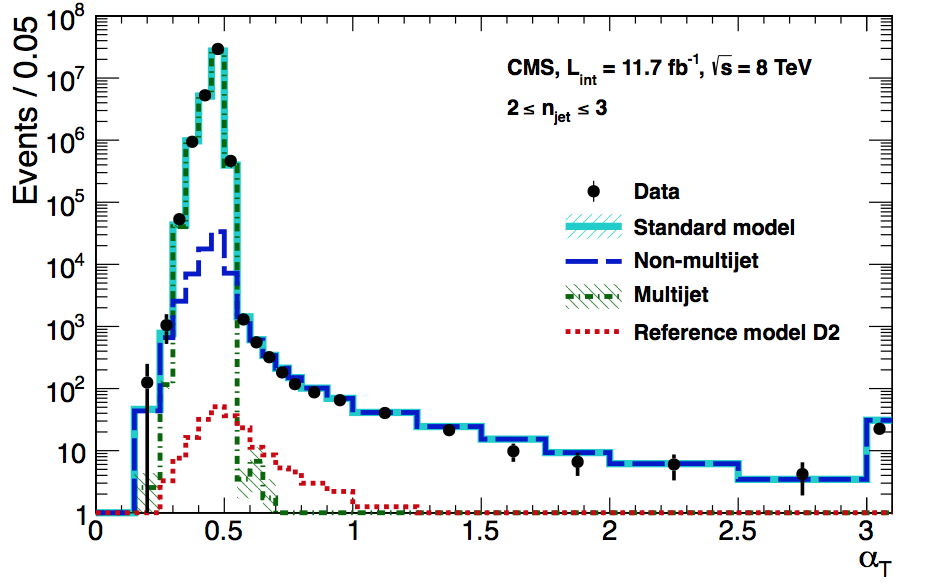
\includegraphics[width=0.8\linewidth]{alphaT1_bkgd}
	\end{center}
	\caption{The $\alpha_T$ values for events with $H_T>375$ GeV and 2 to 3 jets that pass all other cuts imposed in the $\alpha_T$ analysis. The green dotted line shows the expected multijet QCD background that can be removed with an appropriate cut on $\alpha_T$ \cite{AlphaT8TeVChatrchyan:2013lya}}
	\label{fig:alphaT}
\end{figure}

\subsection{The \boldmath $\alpha_T$ analysis}

The only genuine source of missing transverse energy ($\cancel{E}_T$) in the SM is electroweak neutrino production. In these cases an associated lepton is simultaneously produced. This background is minimised by vetoing any events with isolated \footnote{A particle is isolated if the energy of other particles within a cone of $R\equiv\sqrt{(\Delta\phi)^2+(\Delta\eta)^2}=0.3$, where $\phi$ is the azimuthal angle and $\eta$ the pseudorapidity, do not add up to a significant proportion of the particle's momentum, typically $~10$\%} leptons of $p_T>10$~GeV. To ensure a fully hadronic final state there is also a veto on photons of $p_T>25$~GeV. Further, to reduce the ``lost lepton'' backgrounds from W~+~jets 
and $t\bar{t}$, events containing single isolated tracks with $p_T >10$~GeV and $|\eta| < 2.5$ are vetoed.
\\\\
Events are also required to contain at least one $p_T>100$~GeV and one $p_T>40$~GeV jet, where the jets are well reconstructed in the central region, $|\eta|<3$. If any jets fall outside the $\eta$ range, the event is vetoed. Significant hadronic activity is selected for by requiring $H_T>200$~GeV. Events are categorised based on the number of jets, the number of jets with a reconstructed b-quark and the value of $H_T$. 
\\\\
Due to the reduction in QCD cross section at high values of $H_T$, the $\alpha_T$ cut is reduced with this variable while keeping a consistent effective $\cancel{H_T}$ value, see Table~\ref{tab:alphat-thresholds}. Additional cleaning cuts on the ratio of $\cancel{H_T}/\cancel{E_T}$ are also required to reduce instances of high $\cancel{H_T}$ caused by jets just falling out of acceptance. Full details of the analysis as carried out on Run~1 data can be found at \cite{AlphaT8TeVChatrchyan:2013lya} and \cite{AlphaT_7TeV_PRLChatrchyan:2011zy}, and ongoing developments for Run~2 at \cite{AN-15-004}.
\\\\

\begin{table}[h!]
  \caption{$\alpha_T$ and (effective) $\cancel{H_T}$ thresholds per $H_T$ bin.\label{tab:alphat-thresholds}}
  \centering
  \footnotesize
  \begin{tabular}{ lcccccc }
    \hline
    \hline
    $H_T$     & 200--250   & 250--300   & 300--350  & 350--400  & 400--800 \\ %& $>$900       \\
    \hline                                                                     
    $alpha_T$      & 0.65       & 0.60       & 0.55      & 0.53      & 0.52     \\  %& 0.505         \\
    "Min $\cancel{H_T}$"   & $\sim$128  & $\sim$138  & $\sim$125 & $\sim$133 & $\sim$137 \\  %& $\sim$126 \\
    \hline
    \hline
  \end{tabular}
\end{table}

\noindent For the prediction of backgrounds and measuring of systematic errors, control samples are defined. These have all the cuts used for the signal selection described above, but require the existence of one or two leptons or a photon. These leptons and photons are ignored in the calculation of any analysis variables. Additionally, in the case of the lepton control sample no, $\alpha_T$ requirement is made.


% $Id: introduction.tex 34630 2013-04-29 22:53:51Z roldeman $

\section{The Large Hadron Collider}
\label{sec:SUSYproduction}

The LHC is a 27km circumference hadron synchrotron built on the Franco-Swiss border \cite{LHCMachine} near Geneva. It ran from 2010 to 2013 colliding protons at centre-of-mass energies $\sqrt{s}=7$ and $8$ TeV (Run 1), with detectors built around the beam collecting up to $23.3$~fb$^{-1}$ of data. Preparations are currently underway for Run 2 of the LHC at a full operating energy of $\sqrt{s}=13$ to $14$ TeV in 2015. This upgrade will have a maximum instantaneous luminosity of $1.6\times10^{34}$~cm$^{-2}$s$^{-1}$, more than twice the peak of $7.7\times10^{33}$~cm$^{-2}$s$^{-1}$ reached in 2012 \cite{LHCLuminosityIPAC13}. With this increase in energy and luminosity, potential for the discovery of new physics at the energy frontier is high.  
\\\\
\subsection{Supersymmetry production at the LHC}
As the LHC is a hadron collider, the highest cross section SUSY production processes occur via the strong force \cite{SUSYprimerMartin:1997ns} \cite{SUSYxsections_NewAspectsof_pp_collisions}. These processes result in the production of squarks and gluinos, the SUSY particles with colour charge. In all favoured SUSY models, these relatively heavy particles decay within the detector to a weakly interacting LSP, usually a neutralino \cite{SUSYPhe_hadronic_states_Farrar:1978xj}. In collisions at the LHC this will appear as several hard jets with unbalanced momentum (missing energy). 
\\\\
To interpret the results of SUSY searches simplified models are used. These models include a smaller number of SUSY particles than the MSSM, but allow the representation of event topologies in a consistent way \cite{SimplifiedModelsAlves:2011wf} \cite{MathiasSUSYthesis}. A simplified model representation of hadronic SUSY production and decay can be seen in Fig.~\ref{fig:simpdecays}.
\begin{figure}
	\begin{center}
		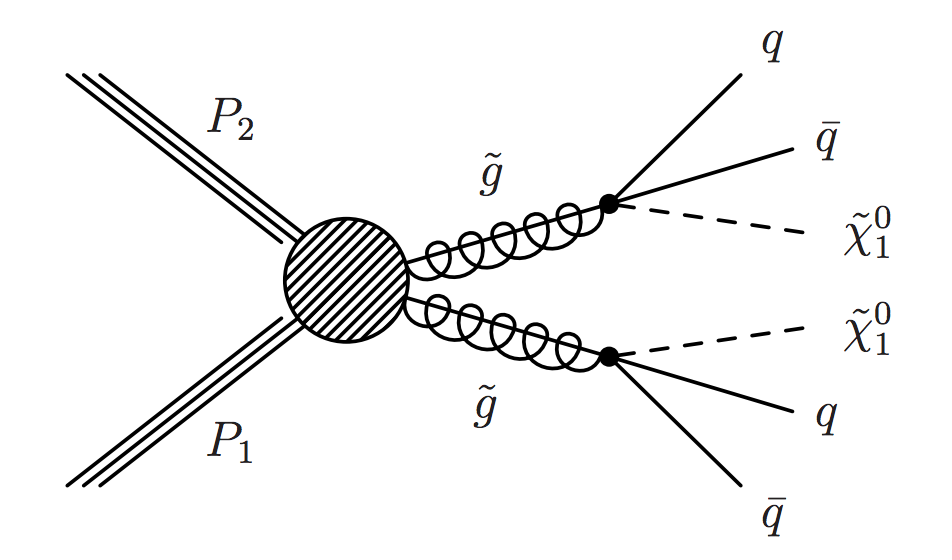
\includegraphics[width=0.4\linewidth]{T1simlifiedpp-gg-qqqqXX}\put(-32,133){(a)}
		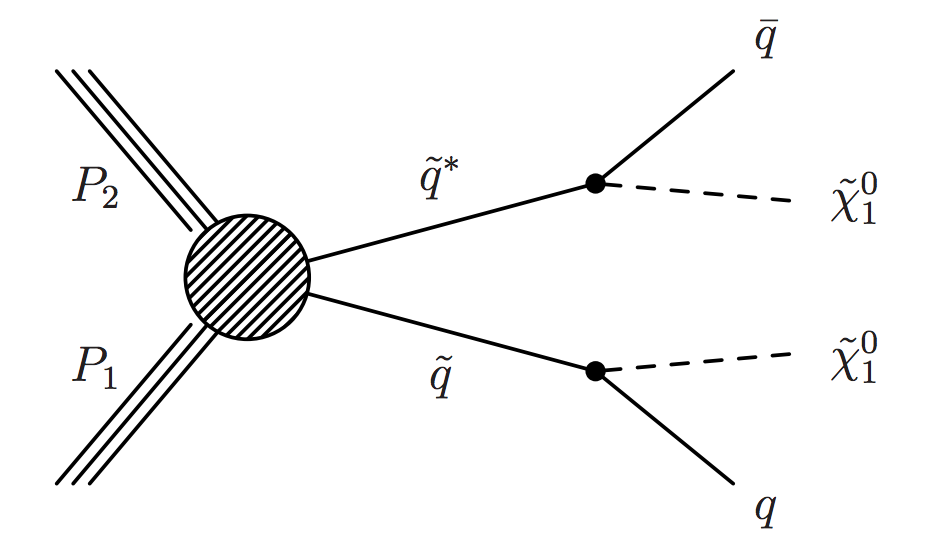
\includegraphics[width=0.4\linewidth]{T2simplifiedpp-qq-qqXX}\put(-32,133){(b)}
	\end{center}
	\caption{Simplified models of SUSY being produced at the LHC and decaying into hadrons plus missing energy \cite{MathiasSUSYthesis}}
	\label{fig:simpdecays}
\end{figure}
\\\\
The $7$ and $8$ TeV run of the LHC has not resulted in any observation of SUSY production as of yet. Instead, limits have been set on the mass of SUSY particles. It is possible that the mass of the SUSY particle has been outside of the energy range of the LHC. With the 2015 upgrade, the cross sections of such supersymmetric particles will increase by at least an order of magnitude, giving a large potential for discovery. It is also possible that the mass splitting of SUSY particles is small, known as compressed spectra. If this is the case the searches at the LHC are not as sensitive, as the energy of the jets produced in the decay to the LSP will be low. This results in a small visible component of missing energy. If SUSY exists at a scale that solves the hierarchy problem with minimal fine tuning, it should be seen at the LHC.

% $Id: introduction.tex 34630 2013-04-29 22:53:51Z roldeman $

\section{The Compact Muon Solenoid detector}
\label{sec:CMS}

The Compact Muon Solenoid (CMS) detector is one of two multipurpose detectors built around proton beam collision points at the LHC. In CMS the results of collisions are measured with a series of subdetectors, built within and around a 3.8T superconducting solenoid, designed to track and record the energy of all non-neutrino SM particles \cite{CMSTechDesign1DetectorPerformance}. A representative view of CMS and its components can be seen in Fig.~\ref{fig:CMS}.
\begin{figure}
	\begin{center}
		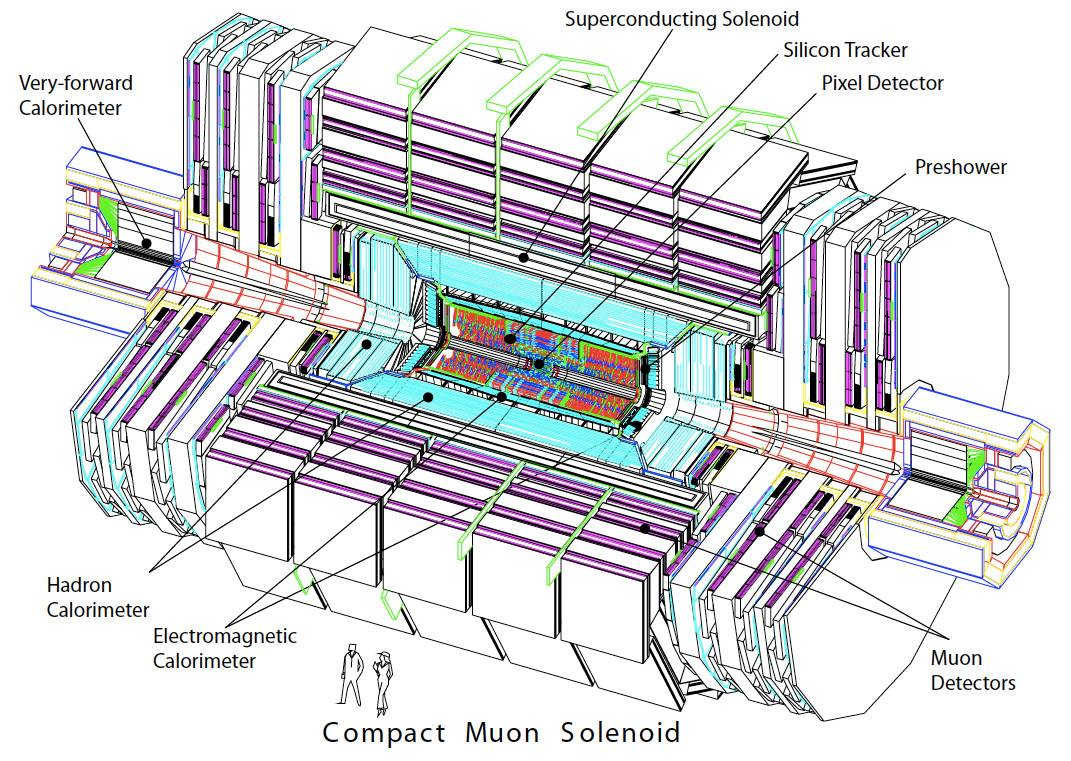
\includegraphics[width=0.8\linewidth]{cms_detector}
	\end{center}
	\caption{An internal view of the Compact Muon Solenoid detector highlighting the key detecting components \cite{CMSTechDesign1DetectorPerformance}}
	\label{fig:CMS}
\end{figure}

\subsection{The Inner Tracking System}
Within the superconducting solenoid is the silicon tracking system that can track \mbox{$p_T>1$~GeV} charged particles with an efficiency greater than $99\%$ \cite{ScienceArticle} \cite{CMSTechDesign1DetectorPerformance}. The Pixel Detector is the high granularity component of the tracking system that sits closest to the interaction point, covering the pseudorapidity region $|\eta|<2.1$ \footnote{$\eta \equiv -ln[tan\frac{\theta}{2}]$, where $\theta$ is measured with respect to the z-axis that points along the beam direction.}. The Silicon Strip Tracker sits around this with barrel and endcap components covering $|\eta|<2.4$. By measuring the curvature of their tracks, charged particle momenta can be measured with an error between $1.5\%$ and $3\%$ for $p_T\sim 100$ GeV \cite{Adam_Elwood_MSci}. The resolution of the trackers is such that the points of origin of event decay products can be inferred within $10$~$\mu$m, allowing the performance of CMS to extend up to very high pileup (number of simultaneous collisions) \cite{CMSTrackPerformance}.

\subsection{The Electromagnetic and Hadronic Calorimeters}
Surrounding the tracking system are the electromagnetic and hadronic calorimeters (ECAL and HCAL). The ECAL is constructed from 75~848 PbWO$_4$ scintillating crystals covering $|\eta|<3$. They are designed to absorb electrons and photons and emit light proportional to the energy deposited. This light is detected by custom photodiodes designed to perform well in high magnetic fields.
\\\\
The HCAL is designed to absorb hadrons and is constructed from brass absorbers interleaved with scintillating plastic tiles covering $|\eta|<3$. The scintillations are read out with hybrid photodiodes via wavelength shifting fibres.
\\\\
In the forward detector regions, the hadronic calorimetry is extended up to $|\eta|<5$ with the Forward Calorimeter, made from steel absorber with quartz scintillating fibre. To also help prevent signal contamination from low energy neutral pions there is a Preshower detector consisting of lead absorbers and silicon microstrips \cite{CMSTechDesign1DetectorPerformance}\cite{Cutajar}.

\subsection{The Muon System}
As muons are unlikely to be absorbed in the ECAL and HCAL, a muon system is built into the iron return yoke that surrounds the solenoid.  This consists of wire chambers containing ionising gas that allows the measurement of muon momenta with a greater than $1\%$ precision \cite{CMS_Overview_Chatrchyan:2008aa}.

\subsection{The Trigger and Data Acquisition System}
The rate of collisions at the LHC is so high that it would be impossible to reconstruct and store the results of all collision events. As the majority of the collisions are soft QCD processes, they are not useful in the search for new physics at the electroweak energy scale. This necessitates a multi-level trigger system that is designed to pick out and store only high centre-of-mass physics processes. The Level 1 Trigger (L1T) is the first component of the trigger system and is made from custom FPGA computational boards situated close to the detector. This uses coarse information from the calorimeters and muon system to reduce the event rate from $20$MHz (during Run 1) to $\sim100$kHz. The data from the subdetectors are then passed to the High Level Trigger (HLT), which uses full detector information to reconstruct the events and reduce the data rate to $\sim1$kHz. The remaining events are then fully reconstructed and stored at various Grid sites \cite{GridTechDesign}.




% $Id: introduction.tex 34630 2013-04-29 22:53:51Z roldeman $

\section{Supersymmetry Searches with the \boldmath $\alpha_T$ Variable}
\label{sec:alphaT}

As motivated in Section~2, it is important to carry out a search for SUSY at the LHC in the hadronic jets plus missing transverse energy, $\cancel{E}_T$, final state. By considering only events with an all hadronic final state, vetoing isolated leptons, electroweak backgrounds can be suppressed. This is particularly important as the only genuine source of $\cancel{E}_T$ in the SM is neutrinos.
\subsection{Definition of \boldmath $\alpha_T$}
The major problem with purely hadronic events is the huge background from multijet events. QCD events can give fake $\cancel{E}_T$ signatures if one or more of the jets are mismeasured in the detector. To overcome this, the dimensionless variable $\alpha_T$ is introduced \cite{AlphaTproposalCMS:2008vya} \cite{AlphaTproposalPhysRevLett.101.221803}. For a dijet system it is defined as:
\begin{equation}
\alpha_T=\frac{E_T^{j_2}}{M_T},
\end{equation}
where $E_T^{j_2}$ is the energy of the lowest energy jet, $M_T=\sqrt{H_T^2-\cancel{H}_T^2}$ is the invariant mass of the dijet system. It is constructed from the jet characterising variables:
\begin{equation}
H_T=\sum_{i=1}^{n_{jet}}E_T^{j_i}, 
\end{equation}
and
\begin{equation}
\cancel{H}_T=|\sum_{i=1}^{n_{jet}}\vec{p}_T^{j_i}|,
\end{equation}
with $n_{jet}$ jets, $j_i$, with transverse momentum $\vec{p}_T^{j_i}$ and transverse energy $E_T^{j_i}$. For events with more than two jets a pseudo dijet system is formed by combining jets. The system chosen is one that minimises $|\Delta H_T|$. This is the difference between the $E_T$ of each pseudo jet, where $E_T$ is the scalar sum of the transverse energies of all the jets in each pseudo jet. This leads to a generalised form of $\alpha_T$ \cite{AlphaT8TeVChatrchyan:2013lya}:
\begin{equation}
\alpha_T=\frac{1}{2}\times\frac{H_T-\Delta H_T}{\sqrt{H_T^2-\cancel{H}_T^2}}
\end{equation}
In the case that two well measured back to back jets are produced by a QCD process, assuming the mass of the jet constituents is much less than the total energy of the jet, $\alpha_T=0.5$. If one of these jets is mismeasured, resulting in fake $\cancel{E}_T$, then $\alpha_T<0.5$. However, if the two jets are recoiling from genuine $\cancel{E}_T$ then $\alpha_T>0.5$. A cut on $\alpha_T$ of around $0.55$ can remove almost all QCD background. The power of this variable to eliminate QCD background can be seen in Fig.~\ref{fig:alphaT}.
\begin{figure}
	\begin{center}
		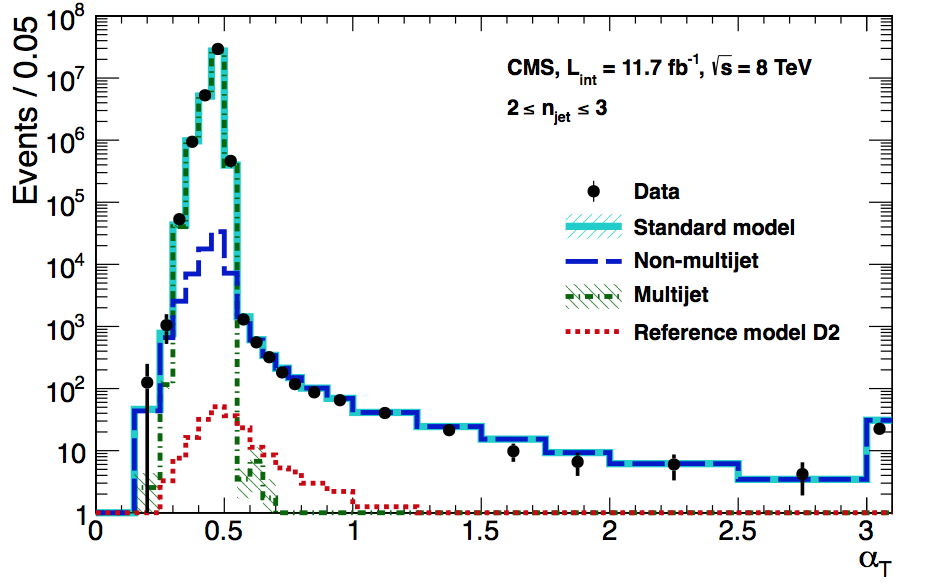
\includegraphics[width=0.8\linewidth]{alphaT1_bkgd}
	\end{center}
	\caption{The $\alpha_T$ values for events with $H_T>375$ GeV and 2 to 3 jets that pass all other cuts imposed in the $\alpha_T$ analysis. The green dotted line shows the expected multijet QCD background that can be removed with an appropriate cut on $\alpha_T$ \cite{AlphaT8TeVChatrchyan:2013lya}}
	\label{fig:alphaT}
\end{figure}
\subsection{The \boldmath $\alpha_T$ analysis}
Events are selected with at least one vertex with $p_T>50$~GeV jets, where the jets are well reconstructed in the central region, $|\eta|<3$. Events with isolated\footnote{A particle is isolated if there are no other particles within a cone of $\sqrt{(\Delta\phi)^2+(\Delta\eta)^2}=0.3$} leptons of $p_T>10$~GeV or photons of $p_T>25$~GeV are vetoed. Events are categorised based on the number of jets, the number of jets with a reconstructed b-quark and the value of $H_T$. This allows for a variable $\alpha_T$ cut based on the category, maximising signal acceptance. Full details of the analysis can be found at \cite{AlphaT8TeVChatrchyan:2013lya} and \cite{AlphaT_7TeV_PRLChatrchyan:2011zy}.


% $Id: introduction.tex 34630 2013-04-29 22:53:51Z roldeman $

\section{The Level 1 Trigger Upgrade}
\label{sec:triggerupgrade}

With the upgrading of the LHC to $\sqrt{s}=13$ to $14$ TeV in 2015 the demands on the trigger are going to be greatly increased, particularly with the instantaneous luminosity increase \cite{TriggerTDR_Tapper:2013yva}. The calculations for triggering on the calorimeters are carried out with a Global Calorimeter Trigger (GCT). The ECAL and HCAL components are split into a $56\times 72$ grid of towers (TT) in $\eta$ and $\phi$ (the azimuthal angle), with each tower covering the area of $5\times5$ ECAL crystals. The GCT in the previous run had limited resources so the towers were grouped into $4\times4$ blocks, known as RCT regions, by the Regional Calorimeter Trigger. This is visually represented in Fig.~\ref{fig:trigger_calorimeter}.
\begin{figure}
	\begin{center}
		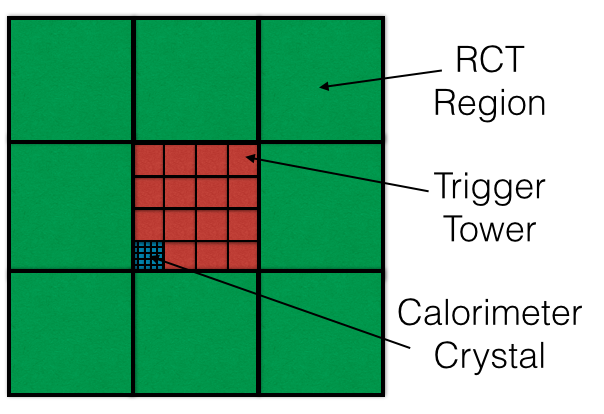
\includegraphics[width=0.4\linewidth]{trigger_calorimeter}
	\end{center}
	\caption{The various calorimeter regions used in algorithms for the L1 trigger}
	\label{fig:trigger_calorimeter}
\end{figure}
\\\\
A key consideration for the L1T is the latency of the algorithms run on the boards. This depends on the algorithms themselves and the boards being used. The latency must be kept low to ensure that each bunch crossing can be processed in as much detail as possible. An upgrade to the trigger is proposed to allow more sophisticated algorithms, while not missing any bunch crossings.
\\\\
\noindent The upgrade to the trigger will come in two stages, each exploiting the recent improvement in the performance of FPGAs and high-speed optical links. Stage 1 will be introduced for the start of Run 2 in 2015 \cite{UCT-TDR}. The basis for Stage 2 will be a Time Multiplexed Trigger (TMT) and will be commissioned in parallel with Stage 1, ready for the 2016 run. 
\\\\
The amount of calorimeter information that can be put into a single FPGA is limited by the IO capacity of the FPGA. To process the full calorimeter data from a single bunch crossing it takes the equivalent of $\sim10$ bunch crossings of time. The GCT deals with this problem by processing different sections of the calorimeter in separate boards. This necessitates duplication of information at the section boundaries. However, by time multiplexing the calorimeter data, it is possible to have 10 FPGAs processing one bunch crossing each with full granularity calorimeter information in each board. This allows much greater flexibility in algorithms as each FPGA has access to all the information available in each event \cite{Baber1_2013} \cite{TMTdemo2012}.

%The algorithms for the trigger
\section{Jet Algorithm for the Level 1 trigger upgrade}
To make use of the L1 trigger upgrades new algorithms must be developed that improve the identification of different particles. With more information available, it is possible to develop more efficient triggers for the various analyses carried out at CMS. The increase in granularity allows the trigger to have a better view of the substructure of energy deposits, allowing the identification of 3 pronged tau jets and isolated electrons that have varying deposits in the ECAL and HCAL for example. 
\\\\
One particular area of potential improvement is in the jet algorithm. During Run 1, the jet candidates were created from a $3\times3$ RCT region sliding window. Candidates in which the central region has the maximum energy are kept as jets. The performance of this algorithm will be severely reduced by the conditions that will be experienced during Run 2. The doubling of the LHC luminosity will result in $\sim$40 instantaneous collisions, or pileup (PU), per bunch crossing. In any bunch crossing with hard scattering event, it is likely that all other simultaneous collisions consist of soft QCD processes, and should therefore be ignored. The process to do this is known as pileup subtraction (PUS), and if done well should remove these soft processes and subtract the contribution they make to the hard physics process under consideration. With the coarse jets available at Run 1 and more limited hardware resources, correcting for the PU is difficult, as one does not want to subtract any interesting physics. The upgrade will therefore aim to carry out PUS and create a jet with a better position resolution.

\subsection{The Stage 2 Jet algorithm}
\label{sec:stage2_jetalgo}
The jet algorithm for Stage 2 of the CMS trigger upgrade operates on the TT-level calorimeter output, with the energy of each TT taken as the sum of the ECAL and HCAL energy. Each TT within $|\eta|<3$ is considered as a candidate. A $9\times9$ square of TTs with the candidate in the centre is constructed. The candidate is vetoed if any of the other TT in the square have an energy deposit of either greater than or greater than or equal to it. The veto condition applied is antisymmetric along the diagonal of the square to prevent TT with the same energy from vetoing one another. A representation of the square considered can be seen in Fig.~\ref{fig:stage2_jetalgo}(a). Any TT that pass this criteria are considered as jet centres, where the jet reconstructed from the TT has the energy equal to the sum of all the towers within the $9\times9$ square. 
\begin{figure}
	\begin{center}
		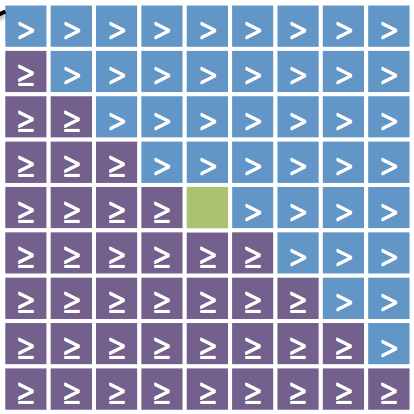
\includegraphics[width=0.3\linewidth]{stage2_jetalgo}\put(-32,143){(a)}
		\hspace{1cm}
		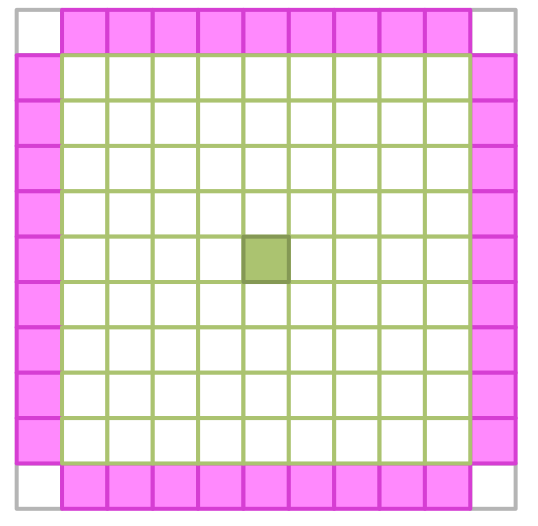
\includegraphics[width=0.3\linewidth]{Donut_plots/donut_region}\put(-32,143){(b)}
	\end{center}
	\caption{(a) The consideration of a Trigger Tower candidate for the Stage 2 Level 1 Trigger jet algorithm. The candidate (green) is vetoed if the energy of the other towers meets the condition shown in the blue and purple towers. (b) The ring considered around a jet when carrying out donut subtraction \cite{jad-l1jets}}
	\label{fig:stage2_jetalgo}
\end{figure}
\\\\
The motivation for the jets having a size of $9\times9$ TT is that the area of each jet is approximately equal to the maximum area allowed for offline jets that are reconstructed using the anti-kt with a maximum radius of 0.4 (AK4) \cite{antiktJetAlgorithm}. This is the algorithm that will be used for offline clustering during Run 2. Taking the highest energy TT as the centre of the jet axis is motivated by the fact that jets are boosted objects with most of their energy in the middle \cite{JetProfile_pileup}. The performance of the algorithm as compared to AK4 can be seen in Fig.~\ref{fig:ak4_comp}.
\begin{figure}
	\begin{center}
		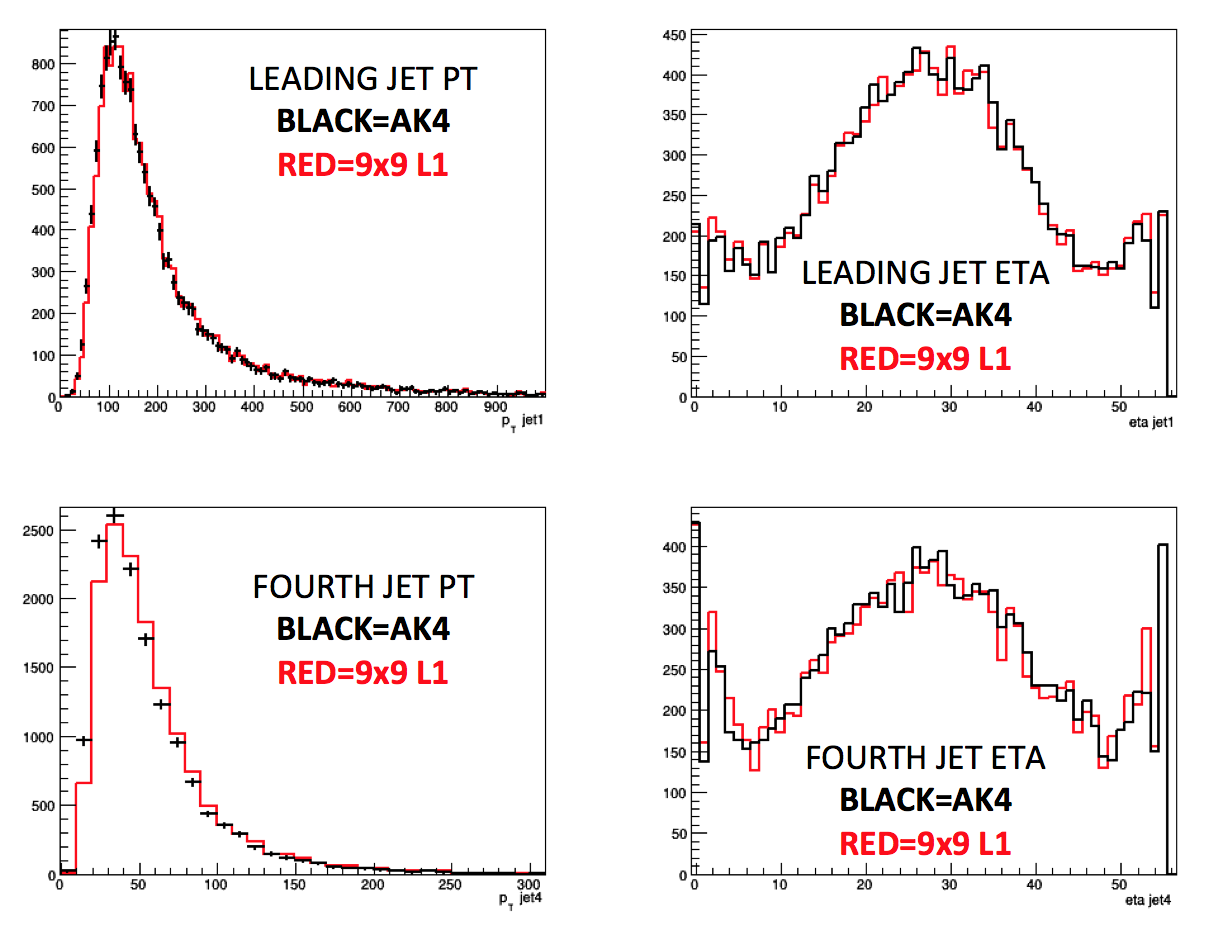
\includegraphics[width=0.8\linewidth]{jet_l1s2_compak4}
	\end{center}
	\caption{A comparison between the proposed Level 1 Stage 2 jet algorithm and anti-kt with R=0.4 with the Trigger Towers as input. These plots are produced from a $t\bar{t}$ Monte Carlo simulation at $13$~TeV with pileup $\sim40$ \cite{jad-l1jets}}
	\label{fig:ak4_comp}
\end{figure}
\\\\
The veto conditions applied on the central TT ensure that no two overlapping jets are reconstructed, avoiding the duplication of energy deposits. However, the algorithm can introduce inefficiencies in very specific jet topologies. In these cases a high energy TT vetoes a medium energy TT which then vetoes a lower energy TT. In this case the medium TT is included in the jet constructed by the high energy TT, however the lower energy TT is lost. This is not usually a problem from the L1 Trigger point of view, as the high energy TT will usually ensure that the event is triggered, despite energy being lost.

%Downsides-> fixed window -> lack of substructure (nsubjettyness)

\subsection{Pileup Subtraction Algorithms}
During or after the creation of L1 jets with the algorithm described in Section~\ref{sec:stage2_jetalgo}, PUS is performed. The purpose of this is to remove jets that originate from soft QCD scattering events and to correct the energy of jets from hard physics processes that have been contaminated by PU. The ideal scenario is one in which the energy of interesting jets is not dependent on the number of collisions during a bunch crossing. Three forms of PUS at L1 are outlined in here and investigated in Section~\ref{sec:jet_algo_performance}. These algorithms are designed to operate on an event-by-event basis, allowing the performance to change dynamically based on differing PU conditions. 
%cite global rho

\subsubsection{Global \boldmath $\rho$}
A prominent method of PUS is to find the average energy per unit area in the calorimeter due to PU, $\rho$, and subtract it from each reconstructed jet. A favoured estimator for this quantity is \cite{global_rho}:
\begin{equation}
\rho\equiv median(\frac{p_{Tj}}{A_j}),
\end{equation}
where $p_{Tj}$ is the transverse momentum of a jet $j$, $A_j$ is its area and the median is taken over all reconstructed jets in an event. This form of PUS is known as global $\rho$ and acts to remove the low energy half of jets in an event and correct the remaining high energy half. It works particularly well high PU cases as $\rho$ is insensitive to fluctuations in the energy of interesting physics events. 
\\\\
A disadvantage of global $\rho$ PUS is the fact that it is non local, it does not account for $\eta$ dependence of PU. In an ideal case PU on average has no $\eta$ dependence, although the response of the calorimeter trigger inputs is not fully independent. It is possible to calculate $\rho$ for particular ranges of $\eta$, local $\rho$, but this method loses robustness as the number of jets that are sampled is lowered for each $\rho$ calculation. 
%At L1, global $\rho$ subtraction also has a latency penalty in hardware, the jets must be found before it can be calculated and subtracted from their energies. Depending on available hardware resources this can present a problem.

\subsubsection{Seed Threshold}
A simple way of reducing the number of soft QCD jets is by introducing an energy threshold on the TT that can form a jet. The TT that is considered for a jet candidate in the algorithm outlined in Section~\ref{sec:stage2_jetalgo} is required to be above a certain energy, known as the seed threshold. This is very easy to implement in hardware, and has the potential to save latency as it reduces the number of jets that need to be made. A disadvantage is that it can kill soft jets that originate from a primary vertex. It is also not $\eta$ dependent, although this possibility is being investigated. For the following studies a seed of $2.5$~GeV (5 in L1 units) was chosen as a benchmark that appeared to kill PU jets without removing jets above 10~GeV from a zero PU $t\bar{t}$ test sample, the optimisation of this seed is to be studied. 

\subsubsection{Donut Subtraction}
The seed threshold does the job of removing PU jets, but does not correct the energy of the reconstructed high energy jets. As hard jets are boosted objects, it is assumed that they most of their energy is deposited very close to the central TT \cite{JetProfile_pileup}. Therefore, in the case of isolated jets, the ring $5$ TT from the centre of the jet can be assumed to contain only PU, see Figure~\ref{fig:stage2_jetalgo}(b). It is therefore proposed to take the energy per unit area in this ring, known as a donut, scale it up by the area of the jet and subtract the resulting energy from the jet. 
\\\\
This approach only works for correcting isolated jets, if one jet is in the vicinity of another the energy in the donut is inflated above that of PU as can be seen in Fig.~\ref{fig:donut_energies}(a). To mitigate this, only the median two $4\times1$ TT strips of the four that make up the donut are used to calculate the PU energy density. This lessens the effect of the contamination, shown in Fig.~\ref{fig:donut_energies}(b). To confirm that this final energy is a measure of the PU in the event, it is plotted against the number of interactions for a Monte Carlo (MC) simulation of $t\bar{t}$ 13~TeV data in Fig.~\ref{fig:donut_nint}. There is a good correlation, implying the donut energy should be a good measure of PU.
\\\\
%donut energy vs nint, response
\begin{figure}
	\begin{center}
		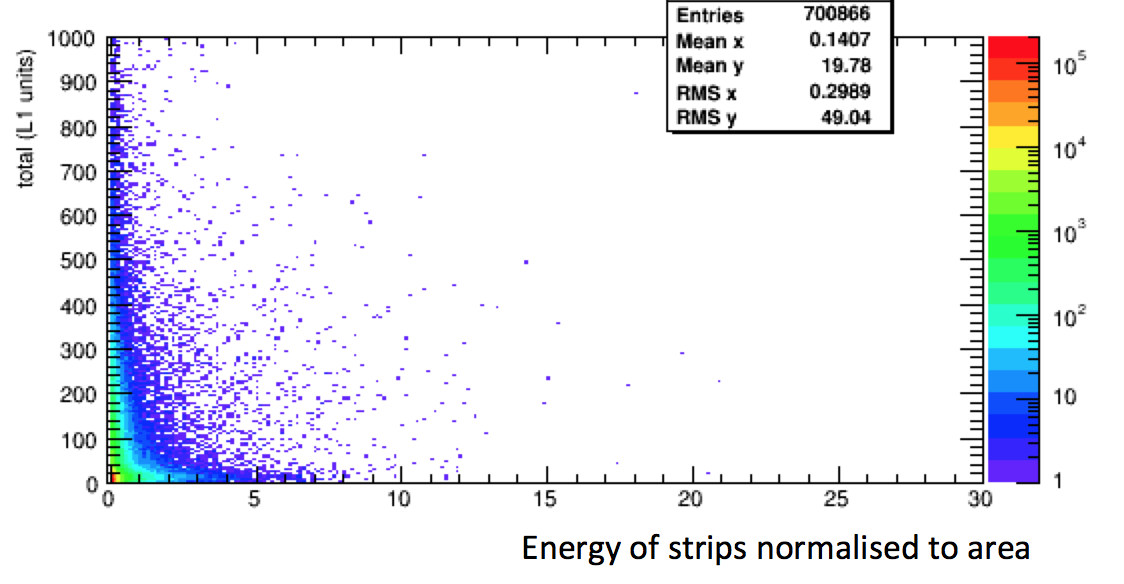
\includegraphics[width=0.5\linewidth]{Donut_plots/noniso_donut_energy}\put(-32,133){(a)}
		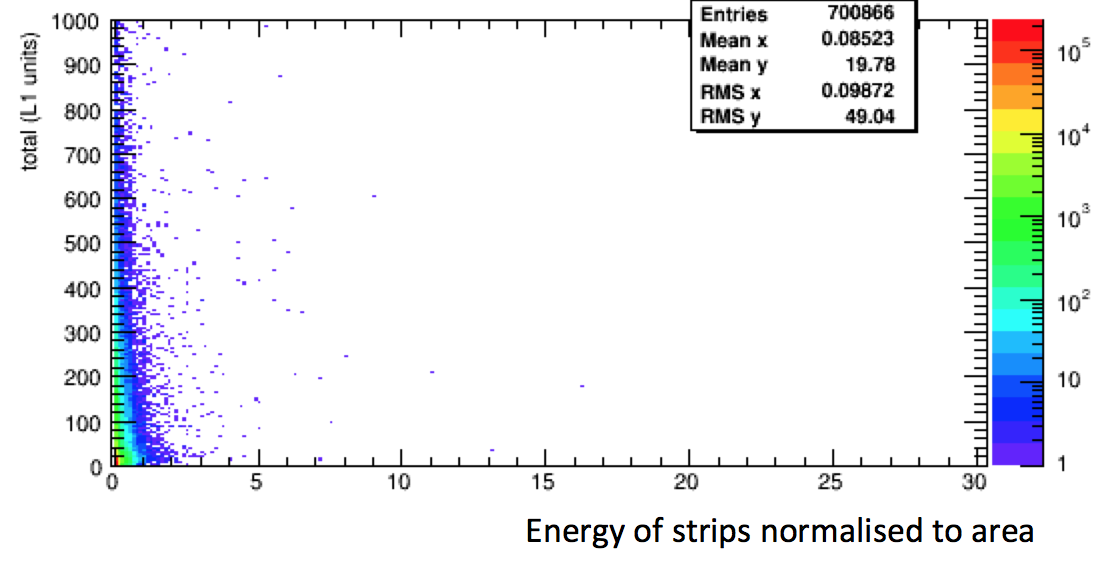
\includegraphics[width=0.5\linewidth]{Donut_plots/noniso_finaldonut_energy}\put(-32,133){(b)}
	\end{center}
	\caption{(a) The energy per unit area in units of $0.5$~GeV/TT of the donut ring taken around the jet. (b) The energy per unit area in units of $0.5$~GeV/TT of the median two strips of the donut ring taken around the jet}
	\label{fig:donut_energies}
\end{figure}
\begin{figure}
	\begin{center}
		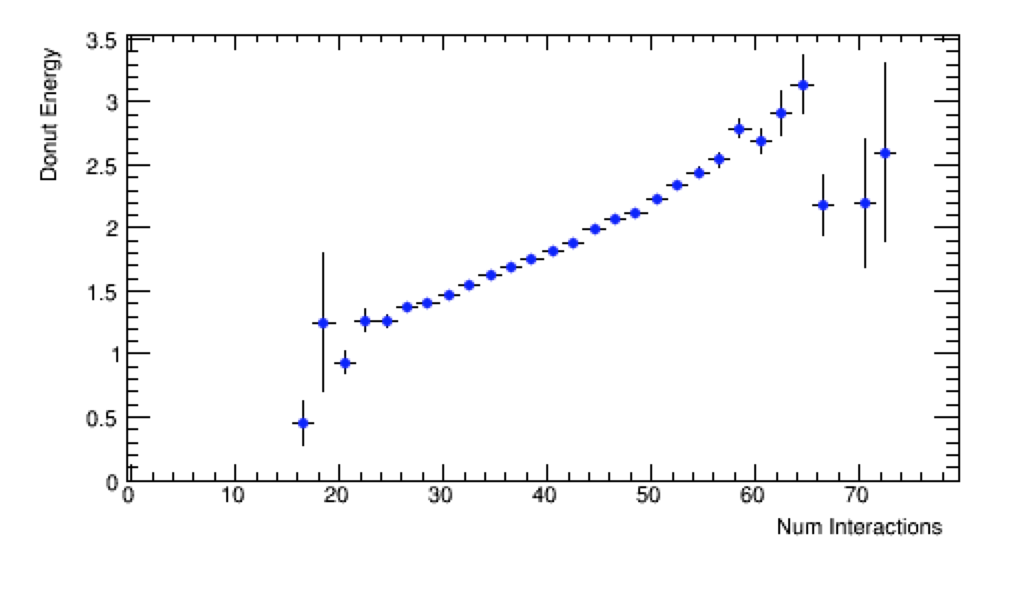
\includegraphics[width=0.6\linewidth]{Donut_plots/donut_nint}
	\end{center}
	\caption{The mean energy of the median two strips of the donut against the number of interactions in an event of $t\bar{t}$ Monte Carlo simulation. Energy is in L1 Units (0.5~GeV)}
	\label{fig:donut_nint}
\end{figure}
\noindent The way L1 hardware carries out the jet finding algorithm, the TT that make up the donut are already available in memory. This means donut subtraction has a very low latency penalty. The main disadvantage is in the sensitivity of the donut energy to fluctuations. Contamination from other close hard jets cause an over subtraction of energy, and in the case that there is no PU within the donut there is an under subtraction. 

\subsection{Performance of the Algorithms}
\label{sec:jet_algo_performance}
The performance of the jet algorithm with the above methods of PUS was tested on 13~TeV MC simulation. A comparison is made to the jets produced by the GCT as it was in 2012. To investigate rates a zero bias neutrino gun sample was used. To test physics performance and compare to AK4 generator level jets (Gen) a $t\bar{t}$ signal sample was used . L1 jets are calibrated with the method as outlined in Section~\ref{sec:pu140_calib}.
%\footnote{/Neutrino\_Pt-2to20\_gun/Fall13dr-tsg\_PU40bx50\_POSTLS162\_V2-v1/GEN-SIM-RAW}
%\footnote{/TT\_Tune4C\_13TeV-pythia8-tauola/Fall13dr-tsg\_PU40bx50\_POSTLS162\_V2-v1/GEN-SIM-RAW}
\\\\
Fig.~\ref{fig:matchingeff} shows the efficiency of Gen jets being reproduced at L1 as a function of their $p_T$. If a Gen jet has a corresponding L1 jet within a radius $R=0.5$ it is counted as matched. This radius is chosen as the distance from the centre of a L1 jet to the corner of its $9\times9$ square. With the proposed Stage 2 jet algorithm, there is close to $100\%$ efficiency above $70$~GeV. The seed appears to be quite aggressive for low $p_T$ jets, but the donut subtraction does not remove any signal jets. The improved granularity greatly improves the performance over the GCT.
%Checked matching to gen, dr 32, inefficiencies caused by algorithm - gct bad
\begin{figure}
	\begin{center}
		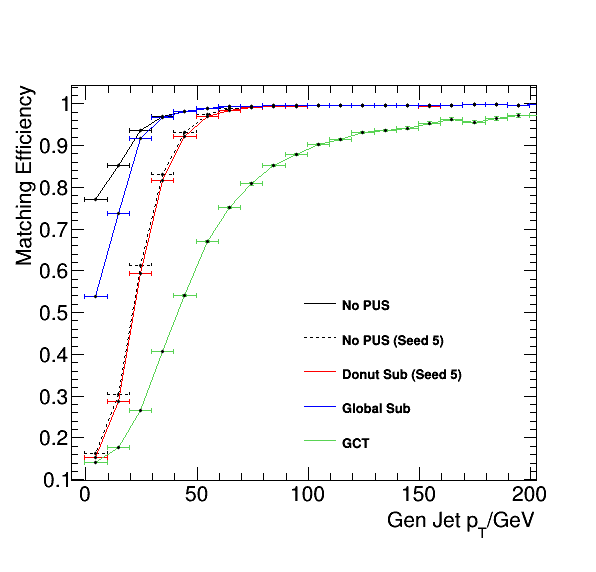
\includegraphics[width=0.6\linewidth]{performance/matchingeff_alljet}
	\end{center}
	\caption{The efficiency with which a Gen jet has a corresponding L1 jet within a radius, $R=0.5$. This is carried out for all Gen jets in 70~000 $t\bar{t}$ events.}
	\label{fig:matchingeff}
\end{figure}
\\\\
\noindent To characterise the energy performance of the L1 jets, turnon curves are plotted in Fig.~\ref{fig:turnons}. These are made by matching the Gen jets to L1 jets, requiring $\Delta R<0.5$ and taking the matched Gen $p_T$ distribution without a cut on L1 jets and one with a cut on the L1 jets, then dividing the two histograms. The fourth leading jet of a $t\bar{t}$ sample is used as it displays the biggest discrepancy between algorithms. By $80$~GeV the PUS doesn't affect the resolution except for donut subtraction which appears to be over subtracting energy in a small number of cases.
\begin{figure}
	\begin{center}
		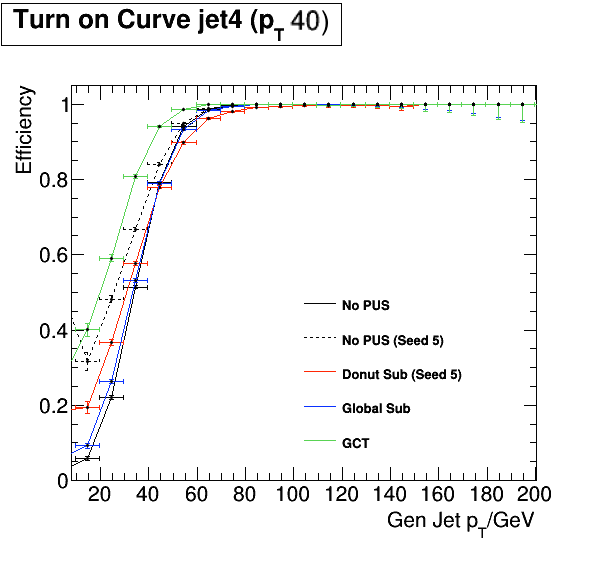
\includegraphics[width=0.5\linewidth]{performance/turnon_jet4_40}\put(-42,203){(a)}
		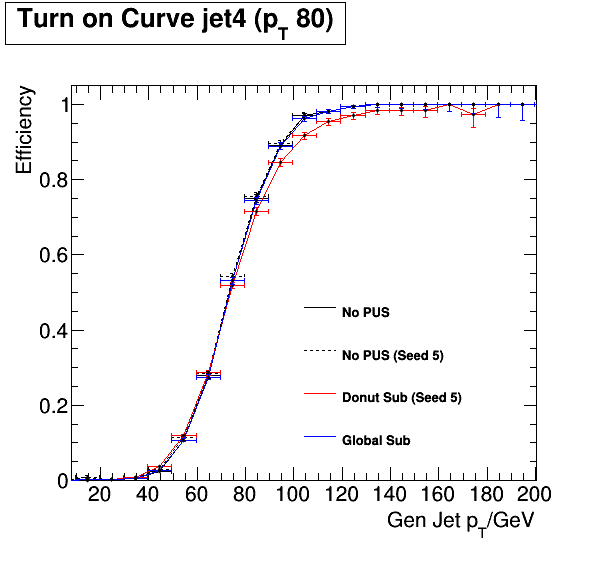
\includegraphics[width=0.5\linewidth]{performance/turnon_jet4_80}\put(-42,203){(b)}
	\end{center}
	\caption{The proportion of remaining Gen jets matched to fourth leading L1 jets after performing a cut on L1 of (a) 40GeV, (b) 80GeV.}
	\label{fig:turnons}
\end{figure}
%turnons - how energy matched to gen - gct bad
\\\\
\noindent To measure the performance of the PUS algorithms removing soft QCD PU jets, the rate against the number of interactions is plotted for the zero bias sample for a representative $p_T$ cut of $30$~GeV, Fig.~\ref{fig:ratenvtx}. The PUS clearly lowers the dependence on the number of interactions and reduces the rate of jets passing the cut, it is performing as it should. It seems that the seed threshold is the most effective at killing soft QCD, with donut subtraction on top not making much difference. GCT jets are incredibly sensitive to PU, further motivating the trigger upgrade.
\begin{figure}
	\begin{center}
		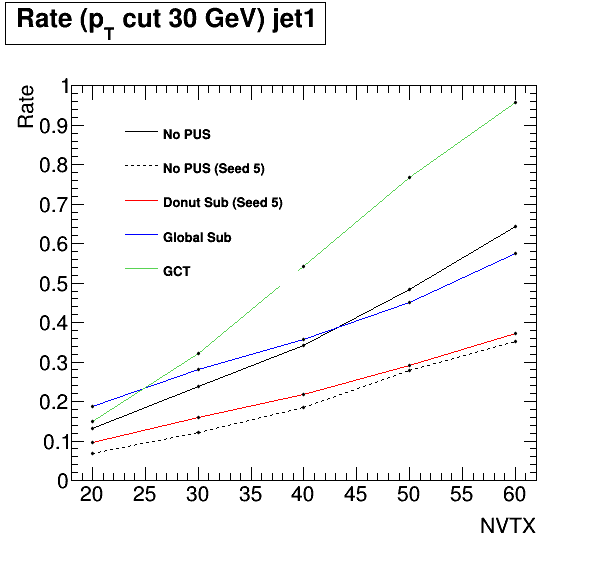
\includegraphics[width=0.5\linewidth]{performance/ratenvtx_neutrino_jet1}\put(-42,203){(a)}
		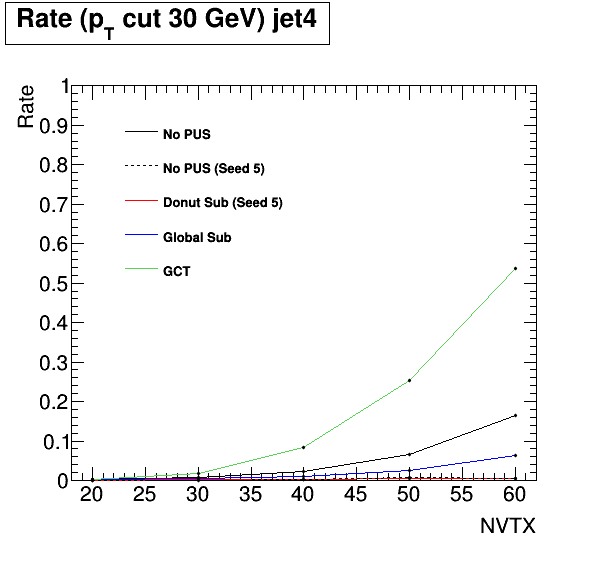
\includegraphics[width=0.5\linewidth]{performance/ratenvtx_neutrino_jet4}\put(-42,203){(b)}
	\end{center}
	\caption{The relative rate of L1 jets with $p_T>30$~GeV after PUS for the leading jet, (a), and fourth leading jet, (b), for $70 000$ zero bias events as a function of the number of interactions (NVTX)}
	\label{fig:ratenvtx}
\end{figure}
%level of soft qcd pileup subtraction- rate vs nvtx
\\\\
\noindent To ensure that the PUS algorithms are not too aggressive, efficiency is plotted against the rate from a zero bias sample given a certain $p_T$ cut. Efficiency is defined as the fraction of events with a lead Gen jet of $p_T>50$~GeV that have a lead L1 jet that is matched to a Gen jet ($\Delta R<0.5$). Ideally the efficiency remains close to one while reducing as much rate as possible. It can be seen in Figure~\ref{fig:rateeff} that for the leading jet very good efficiency is retained in all cases, with the fluctuations in donut subtraction affecting it.
\begin{figure}
	\begin{center}
		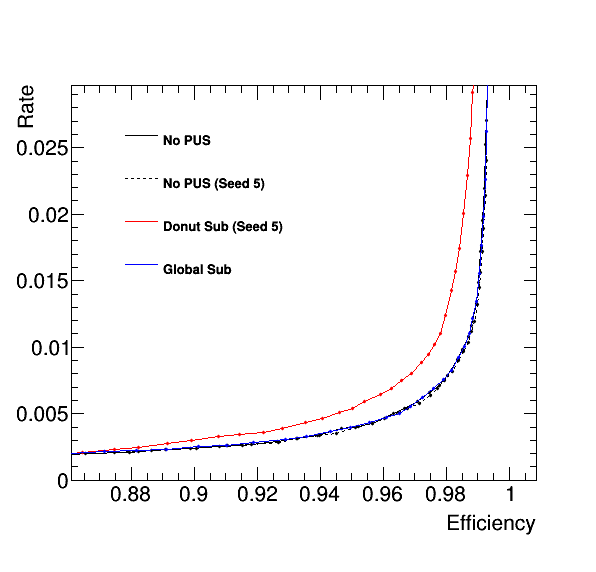
\includegraphics[width=0.6\linewidth]{performance/jet1RateEff}
	\end{center}
	\caption{The normalised rate against efficiency for various PUS schemes. Efficiency is defined as the fraction of events with a lead Gen jet of $p_T>50$~GeV that have a lead L1 jet that is matched to a Gen jet (dR<0.5). Based on a $t\bar{t}$ and zero bias sample.}
	\label{fig:rateeff}
\end{figure}
%\begin{figure}
%	\begin{center}
%		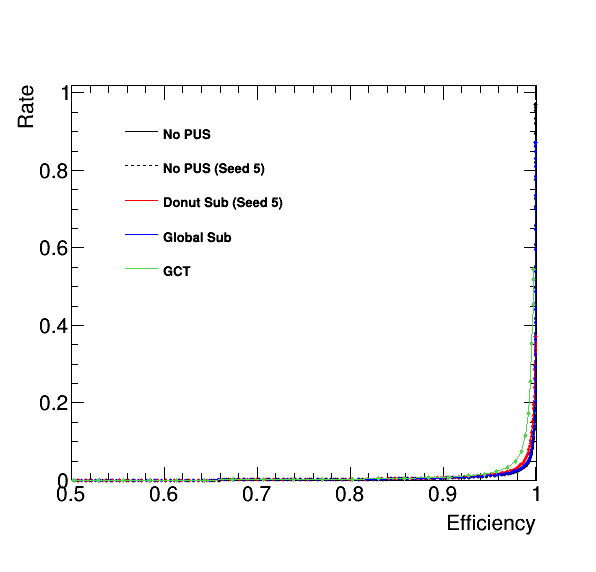
\includegraphics[width=0.5\linewidth]{performance/rateseff_jet1}\put(-42,203){(a)}
%		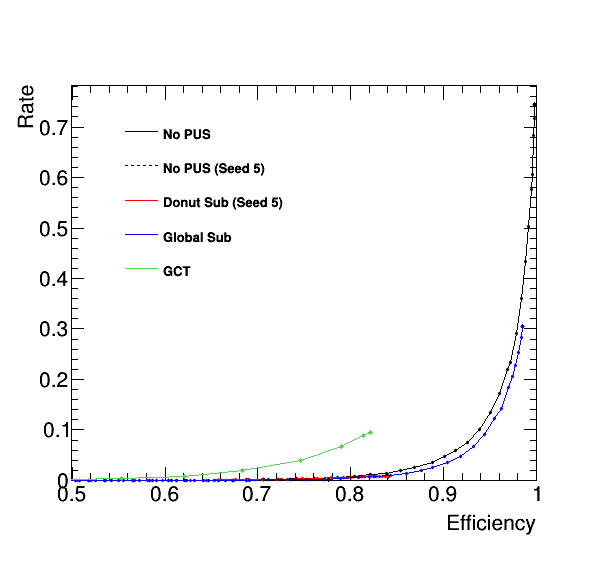
\includegraphics[width=0.5\linewidth]{performance/rateseff_jet4}\put(-42,203){(b)}
% 	\end{center}
%	\caption{Given a particular $p_T$ cut on a level 1 jet the proportion of remaining leading, (a), and fourth %leading, (b), jets is plotted for a zero bias sample against a $t\bar{t}$ sample. The rate is represented by the %zero bias sample and the efficiency by the $t\bar{t}$}
%	\label{fig:rateeff}
%\end{figure}
%maintaining signal- rateseff
\\\\
\noindent The other purpose of PUS is to correct the energy of L1 jets contaminated with PU. The resolution of the jets as compared to Gen is defined as $\frac{p_T^{L1}-p_T^{Gen}}{p_T^{Gen}}$, being zero for perfect agreement. The PUS should act to remove the dependence of the resolution on the number of interactions in an event. In Figure~\ref{fig:resolution} it can be seen that the donut and global $\rho$ subtraction do flatten out the resolution for a representative bin of $p_T$ and $\eta$, whereas the seed on its own does not. 
\begin{figure}
	\begin{center}
		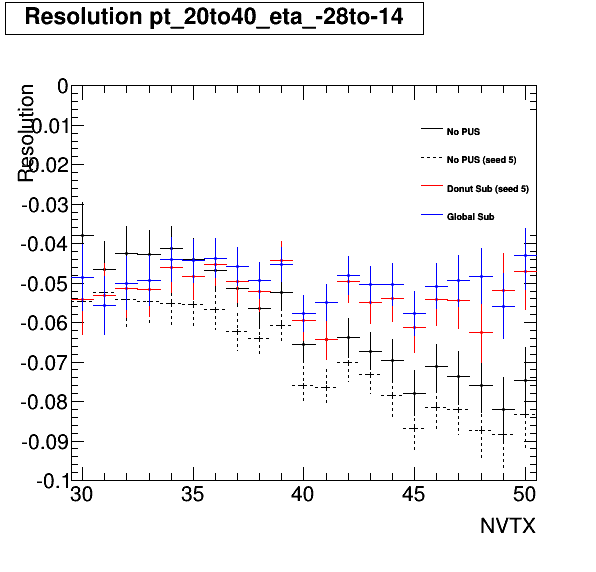
\includegraphics[width=0.6\linewidth]{performance/pt_20to40_eta_-28to-14}
	\end{center}
	\caption{The resolution of L1 jets with $20<p_T<40$~GeV and with $-3<\eta<-1.2$ as a function of the number of interactions (NVTX)}
	\label{fig:resolution}
\end{figure}
%correcting hard jets- response
\\\\
\noindent As a final performance test, the $H_T$ and $\cancel{H}_T$ as defined in Section~\ref{sec:alphaT} are plotted. If the PUS is too aggressive the $H_T$ will be too low when compared to Gen, or too high if it under subtracts. Figure~\ref{fig:htmht} shows that jets with a seed threshold most closely reproduce the $H_T$. Overall the PUS methods are under subtracting, however. The PUS does not improve the $\cancel{H}_T$ distribution, this is expected in the case that PU is distributed evenly.
\begin{figure}
	\begin{center}
		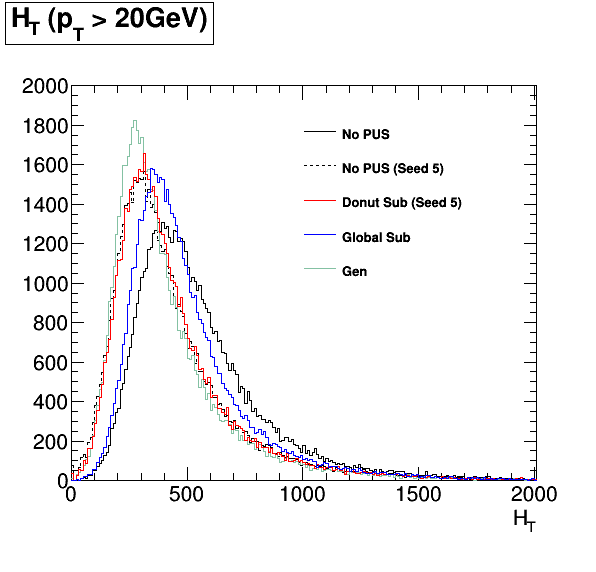
\includegraphics[width=0.5\linewidth]{performance/ht_ttbar}\put(-42,203){(a)}
		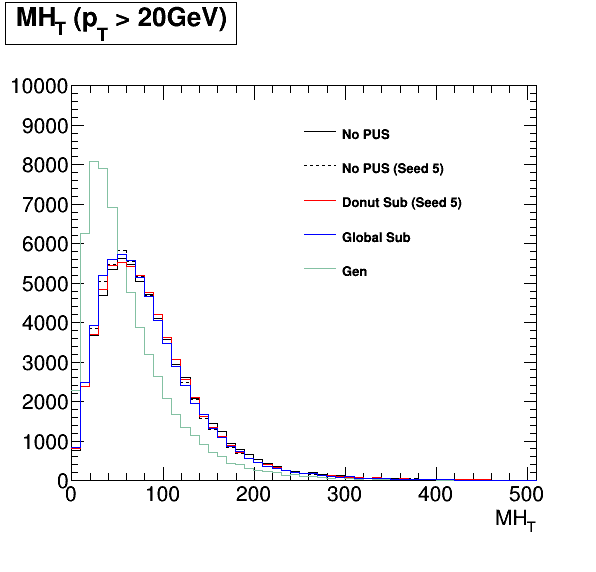
\includegraphics[width=0.5\linewidth]{performance/mht_ttbar}\put(-42,203){(b)}
	\end{center}
	\caption{(a) The distribution of the total energy of jets in each event ($H_T$). (b) The distribution of the missing momentum of jets in an event ($\cancel{H}_T$).}
	\label{fig:htmht}
\end{figure}
%not killing important jets- ht mht
\\\\
\noindent The proposed Stage 2 jet algorithm performs well with respect to the previous GCT algorithm. With the introduction of PUS, the more challenging conditions at 13TeV in Run 2 can start to be tamed. The rate of reconstructed jets can be reduced without sacrificing too much efficiency. Global subtraction and donut subtraction both help to remove the dependence of the energy of signal jets on PU. Due to fluctuations in the donut subtraction, the efficiency takes a hit, but it is better at reproducing the $H_T$ distribution than global $\rho$. This is just the beginning of the investigation of PUS for L1 jets, further investigation is required to optimise the parameters used and compare to other PUS schemes.
%conclusion

\section{Level 1 Jet Calibration for the High Luminosity LHC}
\label{sec:pu140_calib}
The inputs to the trigger do not exactly represent the offline quantities and the L1 jets have an more rigid size than the simulated Gen jets. By correcting the energy of the L1 jets through calibration it is possible to scale there energy to be closer to that of the Gen jets in an event \cite{l1jet-calibration}. It was necessary to produce a set of calibrations for L1 jets made with simulated data for the High Luminosity upgrade of the LHC, with PU of $\sim140$ per bunch crossing, for studies on the upgrade.
\\\\
To perform the calibration, L1 jets are matched to Gen jets produced from MC truth quantities (required to have $\Delta R<0.3$) for a collection of MC simulated events. For a particular bin of Gen $p_T$, a Gaussian is fit to the distribution of L1 jet $p_T$, giving a mean and its standard deviation. This value is plotted on the $x$ axis of the plot in Fig.~\ref{fig:calibfit}. The $y$ value is found by fitting in the same bin the ratio of the Gen and L1 $p_T$. The result is a set of points that can be fit with an appropriate function. To calibrate L1 jets in the future, the correction factor can be calculated by reading off the value of the fit function at a certain L1 $p_T$. 
\\\\
The performance of this calibration can be seen in Fig.~\ref{fig:calibclosure}. In this case the calibration is effective down to around $30$~GeV. This is expected as the fit was only valid until this value. In high PU samples the low energy L1 jets are heavily contaminated. This results in the Gen jets not being matched to the correct corresponding L1 jet, characterised by the turn over in the ratio as the $p_T$ decreases.
%why calibrate
%calibration theory- fit
\begin{figure}
	\begin{center}
		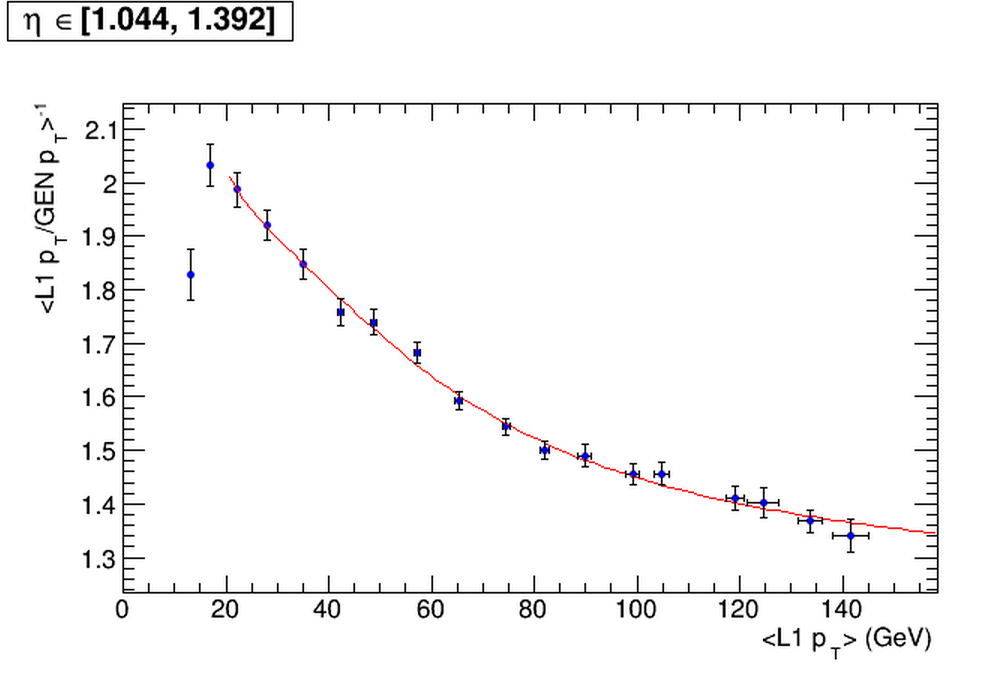
\includegraphics[width=0.6\linewidth]{pu140_calibrationfit}
	\end{center}
	\caption{A fit to the L1 $p_T$ against its ratio with Gen for a particular $\eta$ bin. This fit is used to calculate calibration factors for the L1 jets.}
	\label{fig:calibfit}
\end{figure}
%explain turnover
%closure test- plots
\begin{figure}
	\begin{center}
		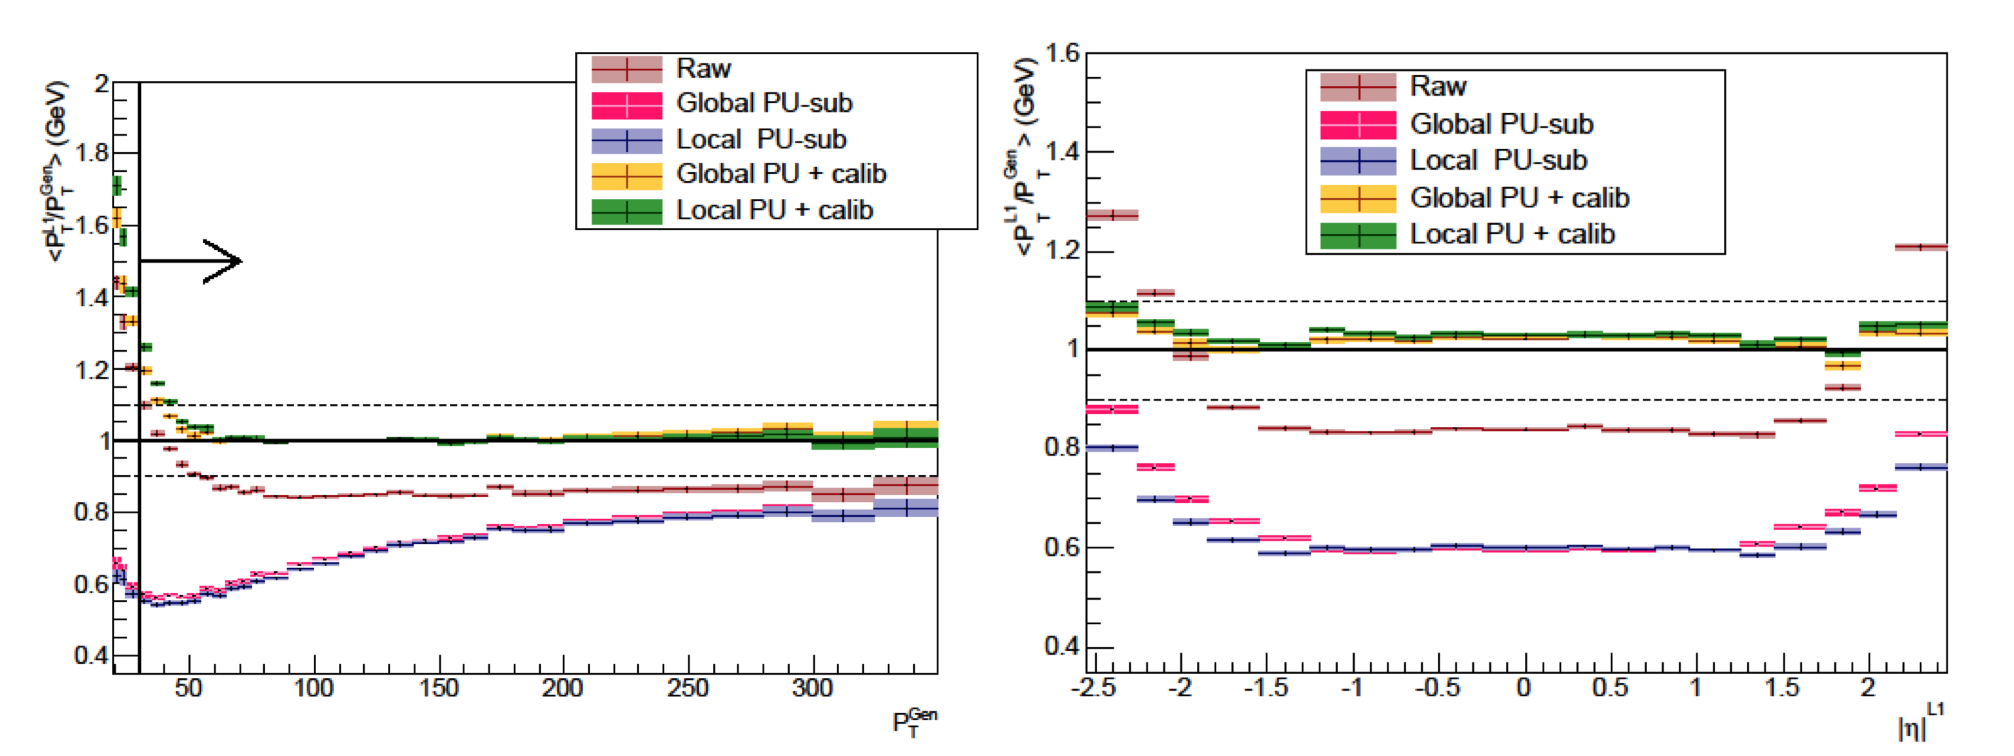
\includegraphics[width=1.0\linewidth]{pu140_calib_closure}
	\end{center}
	\caption{The ratio of L1 jets with Gen before and after they are calibrated, demonstrating the effectiveness of the calibration \cite{nick-pu140calib}}
	\label{fig:calibclosure}
\end{figure}


\section{Conclusions and further work}
\label{sec:conclusion}

The $\alpha_T$ analysis, investigates an important production channel of electroweak scale SUSY. The preparations of the $\alpha_T$ analysis framework for Run~2 of the LHC is nearing completion. Several analysis optimisations have been carried out, improving the sensitivity of the analysis on bench mark SUSY models. Along with this, the effect of new physics object reconstruction algorithms on the analysis have been investigated. In general a moderate improvement is observed.
\\\\
Further work is required to fully understand the implications of the categorisation of events by $\cancel{H_T}$. The change of the systematic error in this dimension, along with the statistical power of the control samples should be fully determined. The aim always being to ensure the $\alpha_T$ analysis is robust and data driven.
\\\\
With the advent of Run~2 data, the analysis methods and frameworks will be tested and validated. Once enough data has been collected, it will be possible to carry out the full analysis. From the preliminary look with $13$~TeV simulated data, it should be possible to start setting limits on the production of new SUSY processes early into Run~2. This gives a potential for discovery around 2016. 


% Do not include this in analysis note and conference reports
%\section*{Acknowledgements}

\noindent The text below are the acknowledgements as approved by the
collaboration board....


%% $Id: appendix.tex 40350 2013-08-07 13:01:10Z tgershon $
% ===============================================================================
% Purpose: appendix to the standard template: standard symbol alises from Ulrik
% Author: Tomasz Skwarnicki
% Created on: 2009-09-24
% ===============================================================================

\clearpage

{\noindent\bf\Large Appendices}

\appendix

\section{Standard References}
\label{sec:StandardReferences}
Below is a list of common references, as
well as a list of all \lhcb publications. 
As they are already in prepared bib files, they can be used as simply as
\texttt{\textbackslash cite\{Alves:2008zz\}} to get the \lhcb detector paper. 
The references are defined in the files \texttt{main.bib},  \texttt{LHCb-PAPER.bib}, \texttt{LHCb-CONF.bib} and \texttt{LHCb-DP.bib} files, with obvious contents.
Each of these have their {\tt LHCb-ZZZ-20XX-0YY} number as their cite code.
If you believe there is a problem with the formatting or
content of one of the entries, then get in contact with the Editorial
Board rather than just editing it in your local file,
since you are likely to need the latest version just before submiting the article.

\begin{center}
  \begin{tabular}{llc}
\hline
Description & \texttt{cite} code & Reference \\
\hline
\lhcb detector & \texttt{Alves:2008zz} & \cite{Alves:2008zz} \\
%% Trigger & \texttt{LHCb-DP-2012-004} & \cite{LHCb-DP-2012-004} \\
%% RICH & \texttt{LHCb-DP-2012-003} & \cite{LHCb-DP-2012-003} \\
PID performance & \texttt{LHCb-PROC-2011-008} & \cite{LHCb-PROC-2011-008} \\
\lhcb simulation & \texttt{LHCb-PROC-2011-006} & \cite{LHCb-PROC-2011-006} \\
PDG 2012 & \texttt{PDG2012} & \cite{PDG2012} \\
HFAG     & \texttt{HFAG} & \cite{HFAG} \\
\pythia6 & \texttt{Sjostrand:2006za} & \cite{Sjostrand:2006za} \\
\lhcb \pythia tuning & \texttt{LHCb-PROC-2010-056} & \cite{LHCb-PROC-2010-056} \\
\geant & \texttt{Allison:2006ve, *Agostinelli:2002hh} & \cite{Allison:2006ve, *Agostinelli:2002hh} \\
\evtgen & \texttt{Lange:2001uf}  & \cite{Lange:2001uf} \\
\photos & \texttt{Golonka:2005pn}  & \cite{Golonka:2005pn} \\
Crystal Ball function & \texttt{Skwarnicki:1986xj} & \cite{Skwarnicki:1986xj} \\
BDT & \texttt{Breiman} & \cite{Breiman} \\
BDT training & \texttt{AdaBoost} & \cite{AdaBoost} \\
HLT2 topo & \texttt{BBDT} & \cite{BBDT} \\
DecayTreeFitter & \texttt{Hulsbergen:2005pu} & \cite{Hulsbergen:2005pu} \\
\sPlot & \texttt{Pivk:2004ty} & \cite{Pivk:2004ty} \\
Punzi's optimization & \texttt{Punzi:2003bu} & \cite{Punzi:2003bu} \\
\hline
  \end{tabular}
\end{center}

\begin{center}
  %% \caption{\small
  %%   LHCb detector performance papers.
  %% }
  %% \label{tab:LHCb-DPs}
  \begin{tabular}{ll}
    \hline
    \texttt{LHCb-DP} number & Title \\
    \hline
    \texttt{LHCb-DP-2013-001}~\cite{LHCb-DP-2013-001} &
    {\small Performance of the muon identification at LHCb} \\
    \texttt{LHCb-DP-2012-005}~\cite{LHCb-DP-2012-005} &
    {\small Radiation damage in the LHCb Vertex Locator} \\
    \texttt{LHCb-DP-2012-004}~\cite{LHCb-DP-2012-004} &
    {\small The \lhcb trigger and its performance in 2011} \\
    \texttt{LHCb-DP-2012-003}~\cite{LHCb-DP-2012-003} &
    {\small Performance of the \lhcb RICH detector at the LHC} \\
    \texttt{LHCb-DP-2012-002}~\cite{LHCb-DP-2012-002} &
    {\small Performance of the LHCb muon system} \\
    \texttt{LHCb-DP-2012-001}~\cite{LHCb-DP-2012-001} &
    {\small Radiation hardness of the LHCb Outer Tracker} \\
    \texttt{LHCb-DP-2011-002}~\cite{LHCb-DP-2011-002} &
    {\small Simulation of machine induced background ...} \\
    \texttt{LHCb-DP-2011-001}~\cite{LHCb-DP-2011-001} &
    {\small Performance of the LHCb muon system with cosmic rays} \\
    \texttt{LHCb-DP-2010-001}~\cite{LHCb-DP-2010-001} &
    {\small First spatial alignment of the LHCb VELO ...} \\
    \hline
  \end{tabular}
\end{center}

\begin{center}
%  \begin{tabular}{l|l}
\begin{longtable}{ll}
\caption{\small
  LHCb-PAPERs (which have their identifier as their cite code).  
  Note that LHCb-PAPER-2011-039 does not exist.
}
\label{tab:LHCb-PAPERs}
\endfirsthead
\multicolumn{2}{c}{ -- continued from previous page.}
\endhead
\endfoot
\endlastfoot
\hline
\texttt{LHCb-PAPER-2013-054}~\cite{LHCb-PAPER-2013-054} &
\texttt{LHCb-PAPER-2013-053}~\cite{LHCb-PAPER-2013-053} \\
\texttt{LHCb-PAPER-2013-052}~\cite{LHCb-PAPER-2013-052} &
\texttt{LHCb-PAPER-2013-051}~\cite{LHCb-PAPER-2013-051} \\
\texttt{LHCb-PAPER-2013-050}~\cite{LHCb-PAPER-2013-050} &
\texttt{LHCb-PAPER-2013-049}~\cite{LHCb-PAPER-2013-049} \\
\texttt{LHCb-PAPER-2013-048}~\cite{LHCb-PAPER-2013-048} &
\texttt{LHCb-PAPER-2013-047}~\cite{LHCb-PAPER-2013-047} \\
\texttt{LHCb-PAPER-2013-046}~\cite{LHCb-PAPER-2013-046} &
\texttt{LHCb-PAPER-2013-045}~\cite{LHCb-PAPER-2013-045} \\
\texttt{LHCb-PAPER-2013-044}~\cite{LHCb-PAPER-2013-044} &
\texttt{LHCb-PAPER-2013-043}~\cite{LHCb-PAPER-2013-043} \\
\texttt{LHCb-PAPER-2013-042}~\cite{LHCb-PAPER-2013-042} &
\texttt{LHCb-PAPER-2013-041}~\cite{LHCb-PAPER-2013-041} \\
\texttt{LHCb-PAPER-2013-040}~\cite{LHCb-PAPER-2013-040} &
\texttt{LHCb-PAPER-2013-039}~\cite{LHCb-PAPER-2013-039} \\
\texttt{LHCb-PAPER-2013-038}~\cite{LHCb-PAPER-2013-038} &
\texttt{LHCb-PAPER-2013-037}~\cite{LHCb-PAPER-2013-037} \\
\texttt{LHCb-PAPER-2013-036}~\cite{LHCb-PAPER-2013-036} &
\texttt{LHCb-PAPER-2013-035}~\cite{LHCb-PAPER-2013-035} \\
\texttt{LHCb-PAPER-2013-034}~\cite{LHCb-PAPER-2013-034} &
\texttt{LHCb-PAPER-2013-033}~\cite{LHCb-PAPER-2013-033} \\
\texttt{LHCb-PAPER-2013-032}~\cite{LHCb-PAPER-2013-032} &
\texttt{LHCb-PAPER-2013-031}~\cite{LHCb-PAPER-2013-031} \\
\texttt{LHCb-PAPER-2013-030}~\cite{LHCb-PAPER-2013-030} &
\texttt{LHCb-PAPER-2013-029}~\cite{LHCb-PAPER-2013-029} \\
\texttt{LHCb-PAPER-2013-028}~\cite{LHCb-PAPER-2013-028} &
\texttt{LHCb-PAPER-2013-027}~\cite{LHCb-PAPER-2013-027} \\
\texttt{LHCb-PAPER-2013-026}~\cite{LHCb-PAPER-2013-026} &
\texttt{LHCb-PAPER-2013-025}~\cite{LHCb-PAPER-2013-025} \\
\texttt{LHCb-PAPER-2013-024}~\cite{LHCb-PAPER-2013-024} &
\texttt{LHCb-PAPER-2013-023}~\cite{LHCb-PAPER-2013-023} \\
\texttt{LHCb-PAPER-2013-022}~\cite{LHCb-PAPER-2013-022} &
\texttt{LHCb-PAPER-2013-021}~\cite{LHCb-PAPER-2013-021} \\
\texttt{LHCb-PAPER-2013-020}~\cite{LHCb-PAPER-2013-020} &
\texttt{LHCb-PAPER-2013-019}~\cite{LHCb-PAPER-2013-019} \\
\texttt{LHCb-PAPER-2013-018}~\cite{LHCb-PAPER-2013-018} &
\texttt{LHCb-PAPER-2013-017}~\cite{LHCb-PAPER-2013-017} \\
\texttt{LHCb-PAPER-2013-016}~\cite{LHCb-PAPER-2013-016} &
\texttt{LHCb-PAPER-2013-015}~\cite{LHCb-PAPER-2013-015} \\
\texttt{LHCb-PAPER-2013-014}~\cite{LHCb-PAPER-2013-014} &
\texttt{LHCb-PAPER-2013-013}~\cite{LHCb-PAPER-2013-013} \\
\texttt{LHCb-PAPER-2013-012}~\cite{LHCb-PAPER-2013-012} &
\texttt{LHCb-PAPER-2013-011}~\cite{LHCb-PAPER-2013-011} \\
\texttt{LHCb-PAPER-2013-010}~\cite{LHCb-PAPER-2013-010} &
\texttt{LHCb-PAPER-2013-009}~\cite{LHCb-PAPER-2013-009} \\
\texttt{LHCb-PAPER-2013-008}~\cite{LHCb-PAPER-2013-008} &
\texttt{LHCb-PAPER-2013-007}~\cite{LHCb-PAPER-2013-007} \\
\texttt{LHCb-PAPER-2013-006}~\cite{LHCb-PAPER-2013-006} &
\texttt{LHCb-PAPER-2013-005}~\cite{LHCb-PAPER-2013-005} \\
\texttt{LHCb-PAPER-2013-004}~\cite{LHCb-PAPER-2013-004} &
\texttt{LHCb-PAPER-2013-003}~\cite{LHCb-PAPER-2013-003} \\
\texttt{LHCb-PAPER-2013-002}~\cite{LHCb-PAPER-2013-002} &
\texttt{LHCb-PAPER-2013-001}~\cite{LHCb-PAPER-2013-001} \\
\hline
\texttt{LHCb-PAPER-2012-057}~\cite{LHCb-PAPER-2012-057} \\
\texttt{LHCb-PAPER-2012-056}~\cite{LHCb-PAPER-2012-056} & 
\texttt{LHCb-PAPER-2012-055}~\cite{LHCb-PAPER-2012-055} \\
\texttt{LHCb-PAPER-2012-054}~\cite{LHCb-PAPER-2012-054} & 
\texttt{LHCb-PAPER-2012-053}~\cite{LHCb-PAPER-2012-053} \\
\texttt{LHCb-PAPER-2012-052}~\cite{LHCb-PAPER-2012-052} & 
\texttt{LHCb-PAPER-2012-051}~\cite{LHCb-PAPER-2012-051} \\
\texttt{LHCb-PAPER-2012-050}~\cite{LHCb-PAPER-2012-050} & 
\texttt{LHCb-PAPER-2012-049}~\cite{LHCb-PAPER-2012-049} \\
\texttt{LHCb-PAPER-2012-048}~\cite{LHCb-PAPER-2012-048} & 
\texttt{LHCb-PAPER-2012-047}~\cite{LHCb-PAPER-2012-047} \\
\texttt{LHCb-PAPER-2012-046}~\cite{LHCb-PAPER-2012-046} & 
\texttt{LHCb-PAPER-2012-045}~\cite{LHCb-PAPER-2012-045} \\
\texttt{LHCb-PAPER-2012-044}~\cite{LHCb-PAPER-2012-044} & 
\texttt{LHCb-PAPER-2012-043}~\cite{LHCb-PAPER-2012-043} \\
\texttt{LHCb-PAPER-2012-042}~\cite{LHCb-PAPER-2012-042} & 
\texttt{LHCb-PAPER-2012-041}~\cite{LHCb-PAPER-2012-041} \\
\texttt{LHCb-PAPER-2012-040}~\cite{LHCb-PAPER-2012-040} & 
\texttt{LHCb-PAPER-2012-039}~\cite{LHCb-PAPER-2012-039} \\
\texttt{LHCb-PAPER-2012-038}~\cite{LHCb-PAPER-2012-038} & 
\texttt{LHCb-PAPER-2012-037}~\cite{LHCb-PAPER-2012-037} \\
\texttt{LHCb-PAPER-2012-036}~\cite{LHCb-PAPER-2012-036} & 
\texttt{LHCb-PAPER-2012-035}~\cite{LHCb-PAPER-2012-035} \\
\texttt{LHCb-PAPER-2012-034}~\cite{LHCb-PAPER-2012-034} & 
\texttt{LHCb-PAPER-2012-033}~\cite{LHCb-PAPER-2012-033} \\
\texttt{LHCb-PAPER-2012-032}~\cite{LHCb-PAPER-2012-032} & 
\texttt{LHCb-PAPER-2012-031}~\cite{LHCb-PAPER-2012-031} \\
\texttt{LHCb-PAPER-2012-030}~\cite{LHCb-PAPER-2012-030} & 
\texttt{LHCb-PAPER-2012-029}~\cite{LHCb-PAPER-2012-029} \\
\texttt{LHCb-PAPER-2012-028}~\cite{LHCb-PAPER-2012-028} & 
\texttt{LHCb-PAPER-2012-027}~\cite{LHCb-PAPER-2012-027} \\
\texttt{LHCb-PAPER-2012-026}~\cite{LHCb-PAPER-2012-026} & 
\texttt{LHCb-PAPER-2012-025}~\cite{LHCb-PAPER-2012-025} \\
\texttt{LHCb-PAPER-2012-024}~\cite{LHCb-PAPER-2012-024} & 
\texttt{LHCb-PAPER-2012-023}~\cite{LHCb-PAPER-2012-023} \\
\texttt{LHCb-PAPER-2012-022}~\cite{LHCb-PAPER-2012-022} & 
\texttt{LHCb-PAPER-2012-021}~\cite{LHCb-PAPER-2012-021} \\
\texttt{LHCb-PAPER-2012-020}~\cite{LHCb-PAPER-2012-020} & 
\texttt{LHCb-PAPER-2012-019}~\cite{LHCb-PAPER-2012-019} \\
\texttt{LHCb-PAPER-2012-018}~\cite{LHCb-PAPER-2012-018} & 
\texttt{LHCb-PAPER-2012-017}~\cite{LHCb-PAPER-2012-017} \\
\texttt{LHCb-PAPER-2012-016}~\cite{LHCb-PAPER-2012-016} & 
\texttt{LHCb-PAPER-2012-015}~\cite{LHCb-PAPER-2012-015} \\
\texttt{LHCb-PAPER-2012-014}~\cite{LHCb-PAPER-2012-014} & 
\texttt{LHCb-PAPER-2012-013}~\cite{LHCb-PAPER-2012-013} \\
\texttt{LHCb-PAPER-2012-012}~\cite{LHCb-PAPER-2012-012} & 
\texttt{LHCb-PAPER-2012-011}~\cite{LHCb-PAPER-2012-011} \\
\texttt{LHCb-PAPER-2012-010}~\cite{LHCb-PAPER-2012-010} & 
\texttt{LHCb-PAPER-2012-009}~\cite{LHCb-PAPER-2012-009} \\
\texttt{LHCb-PAPER-2012-008}~\cite{LHCb-PAPER-2012-008} & 
\texttt{LHCb-PAPER-2012-007}~\cite{LHCb-PAPER-2012-007} \\
\texttt{LHCb-PAPER-2012-006}~\cite{LHCb-PAPER-2012-006} & 
\texttt{LHCb-PAPER-2012-005}~\cite{LHCb-PAPER-2012-005} \\
\texttt{LHCb-PAPER-2012-004}~\cite{LHCb-PAPER-2012-004} & 
\texttt{LHCb-PAPER-2012-003}~\cite{LHCb-PAPER-2012-003} \\
\texttt{LHCb-PAPER-2012-002}~\cite{LHCb-PAPER-2012-002} & 
\texttt{LHCb-PAPER-2012-001}~\cite{LHCb-PAPER-2012-001} \\
\hline
\texttt{LHCb-PAPER-2011-045}~\cite{LHCb-PAPER-2011-045} & 
\texttt{LHCb-PAPER-2011-044}~\cite{LHCb-PAPER-2011-044} \\
\texttt{LHCb-PAPER-2011-043}~\cite{LHCb-PAPER-2011-043} & 
\texttt{LHCb-PAPER-2011-042}~\cite{LHCb-PAPER-2011-042} \\
\texttt{LHCb-PAPER-2011-041}~\cite{LHCb-PAPER-2011-041} & 
\texttt{LHCb-PAPER-2011-040}~\cite{LHCb-PAPER-2011-040} \\
% \texttt{LHCb-PAPER-2011-039}~\cite{LHCb-PAPER-2011-039} &
\texttt{LHCb-PAPER-2011-038}~\cite{LHCb-PAPER-2011-038} &
\texttt{LHCb-PAPER-2011-037}~\cite{LHCb-PAPER-2011-037} \\
\texttt{LHCb-PAPER-2011-036}~\cite{LHCb-PAPER-2011-036} &
\texttt{LHCb-PAPER-2011-035}~\cite{LHCb-PAPER-2011-035} \\
\texttt{LHCb-PAPER-2011-034}~\cite{LHCb-PAPER-2011-034} &
\texttt{LHCb-PAPER-2011-033}~\cite{LHCb-PAPER-2011-033} \\
\texttt{LHCb-PAPER-2011-032}~\cite{LHCb-PAPER-2011-032} & 
\texttt{LHCb-PAPER-2011-031}~\cite{LHCb-PAPER-2011-031} \\
\texttt{LHCb-PAPER-2011-031}~\cite{LHCb-PAPER-2011-030} &
\texttt{LHCb-PAPER-2011-029}~\cite{LHCb-PAPER-2011-029} \\
\texttt{LHCb-PAPER-2011-028}~\cite{LHCb-PAPER-2011-028} &
\texttt{LHCb-PAPER-2011-027}~\cite{LHCb-PAPER-2011-027} \\
\texttt{LHCb-PAPER-2011-026}~\cite{LHCb-PAPER-2011-026} &
\texttt{LHCb-PAPER-2011-025}~\cite{LHCb-PAPER-2011-025} \\
\texttt{LHCb-PAPER-2011-024}~\cite{LHCb-PAPER-2011-024} &
\texttt{LHCb-PAPER-2011-023}~\cite{LHCb-PAPER-2011-023} \\
\texttt{LHCb-PAPER-2011-023}~\cite{LHCb-PAPER-2011-022} &
\texttt{LHCb-PAPER-2011-021}~\cite{LHCb-PAPER-2011-021} \\
\texttt{LHCb-PAPER-2011-020}~\cite{LHCb-PAPER-2011-020} &
\texttt{LHCb-PAPER-2011-019}~\cite{LHCb-PAPER-2011-019} \\
\texttt{LHCb-PAPER-2011-018}~\cite{LHCb-PAPER-2011-018} &
\texttt{LHCb-PAPER-2011-017}~\cite{LHCb-PAPER-2011-017} \\
\texttt{LHCb-PAPER-2011-016}~\cite{LHCb-PAPER-2011-016} &
\texttt{LHCb-PAPER-2011-015}~\cite{LHCb-PAPER-2011-015} \\
\texttt{LHCb-PAPER-2011-014}~\cite{LHCb-PAPER-2011-014} &
\texttt{LHCb-PAPER-2011-013}~\cite{LHCb-PAPER-2011-013} \\
\texttt{LHCb-PAPER-2011-012}~\cite{LHCb-PAPER-2011-012} &
\texttt{LHCb-PAPER-2011-011}~\cite{LHCb-PAPER-2011-011} \\
\texttt{LHCb-PAPER-2011-010}~\cite{LHCb-PAPER-2011-010} &
\texttt{LHCb-PAPER-2011-009}~\cite{LHCb-PAPER-2011-009} \\
\texttt{LHCb-PAPER-2011-008}~\cite{LHCb-PAPER-2011-008} &
\texttt{LHCb-PAPER-2011-007}~\cite{LHCb-PAPER-2011-007} \\
\texttt{LHCb-PAPER-2011-006}~\cite{LHCb-PAPER-2011-006} &
\texttt{LHCb-PAPER-2011-005}~\cite{LHCb-PAPER-2011-005} \\
\texttt{LHCb-PAPER-2011-004}~\cite{LHCb-PAPER-2011-004} &
\texttt{LHCb-PAPER-2011-003}~\cite{LHCb-PAPER-2011-003} \\
\texttt{LHCb-PAPER-2011-002}~\cite{LHCb-PAPER-2011-002} &
\texttt{LHCb-PAPER-2011-001}~\cite{LHCb-PAPER-2011-001} \\
\hline
\texttt{LHCb-PAPER-2010-002}~\cite{LHCb-PAPER-2010-002} &
\texttt{LHCb-PAPER-2010-001}~\cite{LHCb-PAPER-2010-001} \\
\hline
%  \end{tabular}
\end{longtable}
\end{center}

Some \lhcb papers quoted together will look
like~\cite{LHCb-PAPER-2011-007,LHCb-PAPER-2011-006,
  LHCb-PAPER-2011-005,LHCb-PAPER-2011-004,LHCb-PAPER-2011-003}.
The combination of CMS and LHCb results on $B^0_{(s)} \to \mumu$ should be cited like~\cite{LHCb-CONF-2013-012}.

\section{Standard symbols}

As explained in Sect.~\ref{sec:typography} this appendix contains standard
typesetting of symbols, particle names, units etc.\ in \lhcb
documents. 

In the file \texttt{lhcb-symbols-def.tex}, which is included, a
large number of symbols is defined. While they can lead to quicker
typing, the main reason is to ensure a uniform notation within a
document and between different \lhcb documents. If a symbol
like \texttt{\textbackslash CP} to typeset \CP violation is available
for a unit, particle name, process or whatever, it should be used.  If
you do not agree with the notation you should ask to get the
definition in \texttt{lhcb-symbols-def.tex} changed rather than just
ignoring it.

All the main particles have been given symbols. The \B mesons are thus
named \Bp, \Bd, \Bs, and \Bc. There is no need to go into math mode to
use particle names, thus saving the typing of many \$ signs. By
default particle names are typeset in italic type to agree with the
PDG preference. To get roman particle
names you can just change 
\texttt{\textbackslash setboolean\{uprightparticles\}\{false\}}
to \texttt{true} at the top of this template.

There is a large number of units typeset that ensures the correct use
of fonts, capitals and spacing. As an example we have
$\mBs=5366.3\pm0.6\mevcc$. Note that \mum is typeset with an upright
$\upmu$, even if the particle names have slanted greek letters.

A set of useful symbols are defined for working groups. More of these
symbols can be included later. As an example in the Rare Decay group
we have several different analyses looking for a measurement of
\Cpeff7 and \Opep7.

% This is an automatically generated appendix to template.tex. 
% When included it will show all the symbols defined in lhcb-symbols-def.tex.
%
% To regenerate with the latest definitions run the script ./listsymbols

\section{List of all symbols}
\label{sec:listofsymbols}
\subsection{Experiments}
\begin{tabular*}{\linewidth}{@{\extracolsep{\fill}}l@{\extracolsep{0.5cm}}l@{\extracolsep{\fill}}l@{\extracolsep{0.5cm}}l@{\extracolsep{\fill}}l@{\extracolsep{0.5cm}}l}
\texttt{\textbackslash lhcb} & \lhcb & \texttt{\textbackslash atlas} & \atlas & \texttt{\textbackslash cms} & \cms \\
\texttt{\textbackslash alice} & \alice & \texttt{\textbackslash babar} & \babar & \texttt{\textbackslash belle} & \belle \\
\texttt{\textbackslash cleo} & \cleo & \texttt{\textbackslash cdf} & \cdf & \texttt{\textbackslash dzero} & \dzero \\
\texttt{\textbackslash aleph} & \aleph & \texttt{\textbackslash delphi} & \delphi & \texttt{\textbackslash opal} & \opal \\
\texttt{\textbackslash lthree} & \lthree & \texttt{\textbackslash sld} & \sld & \texttt{\textbackslash cern} & \cern \\
\texttt{\textbackslash lhc} & \lhc & \texttt{\textbackslash lep} & \lep & \texttt{\textbackslash tevatron} & \tevatron \\
\end{tabular*}

\subsubsection{LHCb sub-detectors and sub-systems}
\begin{tabular*}{\linewidth}{@{\extracolsep{\fill}}l@{\extracolsep{0.5cm}}l@{\extracolsep{\fill}}l@{\extracolsep{0.5cm}}l@{\extracolsep{\fill}}l@{\extracolsep{0.5cm}}l}
\texttt{\textbackslash velo} & \velo & \texttt{\textbackslash rich} & \rich & \texttt{\textbackslash richone} & \richone \\
\texttt{\textbackslash richtwo} & \richtwo & \texttt{\textbackslash ttracker} & \ttracker & \texttt{\textbackslash intr} & \intr \\
\texttt{\textbackslash st} & \st & \texttt{\textbackslash ot} & \ot & \texttt{\textbackslash spd} & \spd \\
\texttt{\textbackslash presh} & \presh & \texttt{\textbackslash ecal} & \ecal & \texttt{\textbackslash hcal} & \hcal \\
\end{tabular*}

\subsection{Particles}
\subsubsection{Leptons}
\begin{tabular*}{\linewidth}{@{\extracolsep{\fill}}l@{\extracolsep{0.5cm}}l@{\extracolsep{\fill}}l@{\extracolsep{0.5cm}}l@{\extracolsep{\fill}}l@{\extracolsep{0.5cm}}l}
\texttt{\textbackslash electron} & \electron & \texttt{\textbackslash en} & \en & \texttt{\textbackslash ep} & \ep \\
\texttt{\textbackslash epm} & \epm & \texttt{\textbackslash epem} & \epem & \texttt{\textbackslash mmu} & \mmu \\
\texttt{\textbackslash mup} & \mup & \texttt{\textbackslash mun} & \mun & \texttt{\textbackslash mumu} & \mumu \\
\texttt{\textbackslash mtau} & \mtau & \texttt{\textbackslash taup} & \taup & \texttt{\textbackslash taum} & \taum \\
\texttt{\textbackslash tautau} & \tautau & \texttt{\textbackslash ellm} & \ellm & \texttt{\textbackslash ellp} & \ellp \\
\texttt{\textbackslash neu} & \neu & \texttt{\textbackslash neub} & \neub & \texttt{\textbackslash neue} & \neue \\
\texttt{\textbackslash neueb} & \neueb & \texttt{\textbackslash neum} & \neum & \texttt{\textbackslash neumb} & \neumb \\
\texttt{\textbackslash neut} & \neut & \texttt{\textbackslash neutb} & \neutb & \texttt{\textbackslash neul} & \neul \\
\texttt{\textbackslash neulb} & \neulb &  \\
\end{tabular*}

\subsubsection{Gauge bosons and scalars}
\begin{tabular*}{\linewidth}{@{\extracolsep{\fill}}l@{\extracolsep{0.5cm}}l@{\extracolsep{\fill}}l@{\extracolsep{0.5cm}}l@{\extracolsep{\fill}}l@{\extracolsep{0.5cm}}l}
\texttt{\textbackslash g} & \g & \texttt{\textbackslash H} & \H & \texttt{\textbackslash Hp} & \Hp \\
\texttt{\textbackslash Hm} & \Hm & \texttt{\textbackslash Hpm} & \Hpm & \texttt{\textbackslash W} & \W \\
\texttt{\textbackslash Wp} & \Wp & \texttt{\textbackslash Wm} & \Wm & \texttt{\textbackslash Wpm} & \Wpm \\
\texttt{\textbackslash Z} & \Z &  \\
\end{tabular*}

\subsubsection{Quarks}
\begin{tabular*}{\linewidth}{@{\extracolsep{\fill}}l@{\extracolsep{0.5cm}}l@{\extracolsep{\fill}}l@{\extracolsep{0.5cm}}l@{\extracolsep{\fill}}l@{\extracolsep{0.5cm}}l}
\texttt{\textbackslash quark} & \quark & \texttt{\textbackslash quarkbar} & \quarkbar & \texttt{\textbackslash qqbar} & \qqbar \\
\texttt{\textbackslash uquark} & \uquark & \texttt{\textbackslash uquarkbar} & \uquarkbar & \texttt{\textbackslash uubar} & \uubar \\
\texttt{\textbackslash dquark} & \dquark & \texttt{\textbackslash dquarkbar} & \dquarkbar & \texttt{\textbackslash ddbar} & \ddbar \\
\texttt{\textbackslash squark} & \squark & \texttt{\textbackslash squarkbar} & \squarkbar & \texttt{\textbackslash ssbar} & \ssbar \\
\texttt{\textbackslash cquark} & \cquark & \texttt{\textbackslash cquarkbar} & \cquarkbar & \texttt{\textbackslash ccbar} & \ccbar \\
\texttt{\textbackslash bquark} & \bquark & \texttt{\textbackslash bquarkbar} & \bquarkbar & \texttt{\textbackslash bbbar} & \bbbar \\
\texttt{\textbackslash tquark} & \tquark & \texttt{\textbackslash tquarkbar} & \tquarkbar & \texttt{\textbackslash ttbar} & \ttbar \\
\end{tabular*}

\subsubsection{Light mesons}
\begin{tabular*}{\linewidth}{@{\extracolsep{\fill}}l@{\extracolsep{0.5cm}}l@{\extracolsep{\fill}}l@{\extracolsep{0.5cm}}l@{\extracolsep{\fill}}l@{\extracolsep{0.5cm}}l}
\texttt{\textbackslash pion} & \pion & \texttt{\textbackslash piz} & \piz & \texttt{\textbackslash pizs} & \pizs \\
\texttt{\textbackslash pip} & \pip & \texttt{\textbackslash pim} & \pim & \texttt{\textbackslash pipm} & \pipm \\
\texttt{\textbackslash pimp} & \pimp & \texttt{\textbackslash kaon} & \kaon & \texttt{\textbackslash Kb} & \Kb \\
\texttt{\textbackslash Kz} & \Kz & \texttt{\textbackslash Kzb} & \Kzb & \texttt{\textbackslash Kp} & \Kp \\
\texttt{\textbackslash Km} & \Km & \texttt{\textbackslash Kpm} & \Kpm & \texttt{\textbackslash Kmp} & \Kmp \\
\texttt{\textbackslash KS} & \KS & \texttt{\textbackslash KL} & \KL & \texttt{\textbackslash Kstarz} & \Kstarz \\
\texttt{\textbackslash Kstarzb} & \Kstarzb & \texttt{\textbackslash Kstar} & \Kstar & \texttt{\textbackslash Kstarb} & \Kstarb \\
\texttt{\textbackslash Kstarp} & \Kstarp & \texttt{\textbackslash Kstarm} & \Kstarm & \texttt{\textbackslash Kstarpm} & \Kstarpm \\
\texttt{\textbackslash Kstarmp} & \Kstarmp & \texttt{\textbackslash etapr} & \etapr &  \\
\end{tabular*}

\subsubsection{Heavy mesons}
\begin{tabular*}{\linewidth}{@{\extracolsep{\fill}}l@{\extracolsep{0.5cm}}l@{\extracolsep{\fill}}l@{\extracolsep{0.5cm}}l@{\extracolsep{\fill}}l@{\extracolsep{0.5cm}}l}
\texttt{\textbackslash D} & \D & \texttt{\textbackslash Db} & \Db & \texttt{\textbackslash Dz} & \Dz \\
\texttt{\textbackslash Dzb} & \Dzb & \texttt{\textbackslash Dp} & \Dp & \texttt{\textbackslash Dm} & \Dm \\
\texttt{\textbackslash Dpm} & \Dpm & \texttt{\textbackslash Dmp} & \Dmp & \texttt{\textbackslash Dstar} & \Dstar \\
\texttt{\textbackslash Dstarb} & \Dstarb & \texttt{\textbackslash Dstarz} & \Dstarz & \texttt{\textbackslash Dstarzb} & \Dstarzb \\
\texttt{\textbackslash Dstarp} & \Dstarp & \texttt{\textbackslash Dstarm} & \Dstarm & \texttt{\textbackslash Dstarpm} & \Dstarpm \\
\texttt{\textbackslash Dstarmp} & \Dstarmp & \texttt{\textbackslash Ds} & \Ds & \texttt{\textbackslash Dsp} & \Dsp \\
\texttt{\textbackslash Dsm} & \Dsm & \texttt{\textbackslash Dspm} & \Dspm & \texttt{\textbackslash Dsmp} & \Dsmp \\
\texttt{\textbackslash Dss} & \Dss & \texttt{\textbackslash Dssp} & \Dssp & \texttt{\textbackslash Dssm} & \Dssm \\
\texttt{\textbackslash Dsspm} & \Dsspm & \texttt{\textbackslash Dssmp} & \Dssmp & \texttt{\textbackslash B} & \B \\
\texttt{\textbackslash Bbar} & \Bbar & \texttt{\textbackslash Bb} & \Bb & \texttt{\textbackslash Bz} & \Bz \\
\texttt{\textbackslash Bzb} & \Bzb & \texttt{\textbackslash Bu} & \Bu & \texttt{\textbackslash Bub} & \Bub \\
\texttt{\textbackslash Bp} & \Bp & \texttt{\textbackslash Bm} & \Bm & \texttt{\textbackslash Bpm} & \Bpm \\
\texttt{\textbackslash Bmp} & \Bmp & \texttt{\textbackslash Bd} & \Bd & \texttt{\textbackslash Bs} & \Bs \\
\texttt{\textbackslash Bsb} & \Bsb & \texttt{\textbackslash Bdb} & \Bdb & \texttt{\textbackslash Bc} & \Bc \\
\texttt{\textbackslash Bcp} & \Bcp & \texttt{\textbackslash Bcm} & \Bcm & \texttt{\textbackslash Bcpm} & \Bcpm \\
\end{tabular*}

\subsubsection{Onia}
\begin{tabular*}{\linewidth}{@{\extracolsep{\fill}}l@{\extracolsep{0.5cm}}l@{\extracolsep{\fill}}l@{\extracolsep{0.5cm}}l@{\extracolsep{\fill}}l@{\extracolsep{0.5cm}}l}
\texttt{\textbackslash jpsi} & \jpsi & \texttt{\textbackslash psitwos} & \psitwos & \texttt{\textbackslash psiprpr} & \psiprpr \\
\texttt{\textbackslash etac} & \etac & \texttt{\textbackslash chiczero} & \chiczero & \texttt{\textbackslash chicone} & \chicone \\
\texttt{\textbackslash chictwo} & \chictwo & \texttt{\textbackslash OneS} & \OneS & \texttt{\textbackslash TwoS} & \TwoS \\
\texttt{\textbackslash ThreeS} & \ThreeS & \texttt{\textbackslash FourS} & \FourS & \texttt{\textbackslash FiveS} & \FiveS \\
\texttt{\textbackslash chic} & \chic &  \\
\end{tabular*}

\subsubsection{Baryons}
\begin{tabular*}{\linewidth}{@{\extracolsep{\fill}}l@{\extracolsep{0.5cm}}l@{\extracolsep{\fill}}l@{\extracolsep{0.5cm}}l@{\extracolsep{\fill}}l@{\extracolsep{0.5cm}}l}
\texttt{\textbackslash proton} & \proton & \texttt{\textbackslash antiproton} & \antiproton & \texttt{\textbackslash neutron} & \neutron \\
\texttt{\textbackslash antineutron} & \antineutron & \texttt{\textbackslash Deltares} & \Deltares & \texttt{\textbackslash Deltaresbar} & \Deltaresbar \\
\texttt{\textbackslash Xires} & \Xires & \texttt{\textbackslash Xiresbar} & \Xiresbar & \texttt{\textbackslash Lz} & \Lz \\
\texttt{\textbackslash Lbar} & \Lbar & \texttt{\textbackslash Lambdares} & \Lambdares & \texttt{\textbackslash Lambdaresbar} & \Lambdaresbar \\
\texttt{\textbackslash Sigmares} & \Sigmares & \texttt{\textbackslash Sigmaresbar} & \Sigmaresbar & \texttt{\textbackslash Omegares} & \Omegares \\
\texttt{\textbackslash Omegaresbar} & \Omegaresbar & \texttt{\textbackslash Lb} & \Lb & \texttt{\textbackslash Lbbar} & \Lbbar \\
\texttt{\textbackslash Lc} & \Lc & \texttt{\textbackslash Lcbar} & \Lcbar &  \\
\end{tabular*}

\subsection{Physics symbols}
\subsubsection{Decays}
\begin{tabular*}{\linewidth}{@{\extracolsep{\fill}}l@{\extracolsep{0.5cm}}l@{\extracolsep{\fill}}l@{\extracolsep{0.5cm}}l@{\extracolsep{\fill}}l@{\extracolsep{0.5cm}}l}
\texttt{\textbackslash BF} & \BF & \texttt{\textbackslash BRvis} & \BRvis & \texttt{\textbackslash BR} & \BR \\
\texttt{\textbackslash decay[2] \textbackslash decay\{\Pa\}\{\Pb \Pc\}} & \decay{\Pa}{\Pb \Pc} & \texttt{\textbackslash ra} & \ra & \texttt{\textbackslash to} & \to \\
\end{tabular*}

\subsubsection{Lifetimes}
\begin{tabular*}{\linewidth}{@{\extracolsep{\fill}}l@{\extracolsep{0.5cm}}l@{\extracolsep{\fill}}l@{\extracolsep{0.5cm}}l@{\extracolsep{\fill}}l@{\extracolsep{0.5cm}}l}
\texttt{\textbackslash tauBs} & \tauBs & \texttt{\textbackslash tauBd} & \tauBd & \texttt{\textbackslash tauBz} & \tauBz \\
\texttt{\textbackslash tauBu} & \tauBu & \texttt{\textbackslash tauDp} & \tauDp & \texttt{\textbackslash tauDz} & \tauDz \\
\texttt{\textbackslash tauL} & \tauL & \texttt{\textbackslash tauH} & \tauH &  \\
\end{tabular*}

\subsubsection{Masses}
\begin{tabular*}{\linewidth}{@{\extracolsep{\fill}}l@{\extracolsep{0.5cm}}l@{\extracolsep{\fill}}l@{\extracolsep{0.5cm}}l@{\extracolsep{\fill}}l@{\extracolsep{0.5cm}}l}
\texttt{\textbackslash mBd} & \mBd & \texttt{\textbackslash mBp} & \mBp & \texttt{\textbackslash mBs} & \mBs \\
\texttt{\textbackslash mBc} & \mBc & \texttt{\textbackslash mLb} & \mLb &  \\
\end{tabular*}

\subsubsection{EW theory, groups}
\begin{tabular*}{\linewidth}{@{\extracolsep{\fill}}l@{\extracolsep{0.5cm}}l@{\extracolsep{\fill}}l@{\extracolsep{0.5cm}}l@{\extracolsep{\fill}}l@{\extracolsep{0.5cm}}l}
\texttt{\textbackslash grpsuthree} & \grpsuthree & \texttt{\textbackslash grpsutw} & \grpsutw & \texttt{\textbackslash grpuone} & \grpuone \\
\texttt{\textbackslash ssqtw} & \ssqtw & \texttt{\textbackslash csqtw} & \csqtw & \texttt{\textbackslash stw} & \stw \\
\texttt{\textbackslash ctw} & \ctw & \texttt{\textbackslash ssqtwef} & \ssqtwef & \texttt{\textbackslash csqtwef} & \csqtwef \\
\texttt{\textbackslash stwef} & \stwef & \texttt{\textbackslash ctwef} & \ctwef & \texttt{\textbackslash gv} & \gv \\
\texttt{\textbackslash ga} & \ga & \texttt{\textbackslash order} & \order & \texttt{\textbackslash ordalph} & \ordalph \\
\texttt{\textbackslash ordalsq} & \ordalsq & \texttt{\textbackslash ordalcb} & \ordalcb &  \\
\end{tabular*}

\subsubsection{QCD parameters}
\begin{tabular*}{\linewidth}{@{\extracolsep{\fill}}l@{\extracolsep{0.5cm}}l@{\extracolsep{\fill}}l@{\extracolsep{0.5cm}}l@{\extracolsep{\fill}}l@{\extracolsep{0.5cm}}l}
\texttt{\textbackslash as} & \as & \texttt{\textbackslash MSb} & \MSb & \texttt{\textbackslash lqcd} & \lqcd \\
\texttt{\textbackslash qsq} & \qsq &  \\
\end{tabular*}

\subsubsection{CKM, CP violation}
\begin{tabular*}{\linewidth}{@{\extracolsep{\fill}}l@{\extracolsep{0.5cm}}l@{\extracolsep{\fill}}l@{\extracolsep{0.5cm}}l@{\extracolsep{\fill}}l@{\extracolsep{0.5cm}}l}
\texttt{\textbackslash eps} & \eps & \texttt{\textbackslash epsK} & \epsK & \texttt{\textbackslash epsB} & \epsB \\
\texttt{\textbackslash epsp} & \epsp & \texttt{\textbackslash CP} & \CP & \texttt{\textbackslash CPT} & \CPT \\
\texttt{\textbackslash rhobar} & \rhobar & \texttt{\textbackslash etabar} & \etabar & \texttt{\textbackslash Vud} & \Vud \\
\texttt{\textbackslash Vcd} & \Vcd & \texttt{\textbackslash Vtd} & \Vtd & \texttt{\textbackslash Vus} & \Vus \\
\texttt{\textbackslash Vcs} & \Vcs & \texttt{\textbackslash Vts} & \Vts & \texttt{\textbackslash Vub} & \Vub \\
\texttt{\textbackslash Vcb} & \Vcb & \texttt{\textbackslash Vtb} & \Vtb &  \\
\end{tabular*}

\subsubsection{Oscillations}
\begin{tabular*}{\linewidth}{@{\extracolsep{\fill}}l@{\extracolsep{0.5cm}}l@{\extracolsep{\fill}}l@{\extracolsep{0.5cm}}l@{\extracolsep{\fill}}l@{\extracolsep{0.5cm}}l}
\texttt{\textbackslash dm} & \dm & \texttt{\textbackslash dms} & \dms & \texttt{\textbackslash dmd} & \dmd \\
\texttt{\textbackslash DG} & \DG & \texttt{\textbackslash DGs} & \DGs & \texttt{\textbackslash DGd} & \DGd \\
\texttt{\textbackslash Gs} & \Gs & \texttt{\textbackslash Gd} & \Gd & \texttt{\textbackslash MBq} & \MBq \\
\texttt{\textbackslash DGq} & \DGq & \texttt{\textbackslash Gq} & \Gq & \texttt{\textbackslash dmq} & \dmq \\
\texttt{\textbackslash GL} & \GL & \texttt{\textbackslash GH} & \GH & \texttt{\textbackslash DGsGs} & \DGsGs \\
\texttt{\textbackslash Delm} & \Delm & \texttt{\textbackslash ACP} & \ACP & \texttt{\textbackslash Adir} & \Adir \\
\texttt{\textbackslash Amix} & \Amix & \texttt{\textbackslash ADelta} & \ADelta & \texttt{\textbackslash phid} & \phid \\
\texttt{\textbackslash sinphid} & \sinphid & \texttt{\textbackslash phis} & \phis & \texttt{\textbackslash betas} & \betas \\
\texttt{\textbackslash sbetas} & \sbetas & \texttt{\textbackslash stbetas} & \stbetas & \texttt{\textbackslash stphis} & \stphis \\
\texttt{\textbackslash sinphis} & \sinphis &  \\
\end{tabular*}

\subsubsection{Tagging}
\begin{tabular*}{\linewidth}{@{\extracolsep{\fill}}l@{\extracolsep{0.5cm}}l@{\extracolsep{\fill}}l@{\extracolsep{0.5cm}}l@{\extracolsep{\fill}}l@{\extracolsep{0.5cm}}l}
\texttt{\textbackslash edet} & \edet & \texttt{\textbackslash erec} & \erec & \texttt{\textbackslash esel} & \esel \\
\texttt{\textbackslash etrg} & \etrg & \texttt{\textbackslash etot} & \etot & \texttt{\textbackslash mistag} & \mistag \\
\texttt{\textbackslash wcomb} & \wcomb & \texttt{\textbackslash etag} & \etag & \texttt{\textbackslash etagcomb} & \etagcomb \\
\texttt{\textbackslash effeff} & \effeff & \texttt{\textbackslash effeffcomb} & \effeffcomb & \texttt{\textbackslash efftag} & \efftag \\
\texttt{\textbackslash effD} & \effD & \texttt{\textbackslash etagprompt} & \etagprompt & \texttt{\textbackslash etagLL} & \etagLL \\
\end{tabular*}

\subsubsection{Key decay channels}
\begin{tabular*}{\linewidth}{@{\extracolsep{\fill}}l@{\extracolsep{0.5cm}}l@{\extracolsep{\fill}}l@{\extracolsep{0.5cm}}l@{\extracolsep{\fill}}l@{\extracolsep{0.5cm}}l}
\texttt{\textbackslash BdToKstmm} & \BdToKstmm & \texttt{\textbackslash BdbToKstmm} & \BdbToKstmm & \texttt{\textbackslash BsToJPsiPhi} & \BsToJPsiPhi \\
\texttt{\textbackslash BdToJPsiKst} & \BdToJPsiKst & \texttt{\textbackslash BdbToJPsiKst} & \BdbToJPsiKst & \texttt{\textbackslash BsPhiGam} & \BsPhiGam \\
\texttt{\textbackslash BdKstGam} & \BdKstGam & \texttt{\textbackslash BTohh} & \BTohh & \texttt{\textbackslash BdTopipi} & \BdTopipi \\
\texttt{\textbackslash BdToKpi} & \BdToKpi & \texttt{\textbackslash BsToKK} & \BsToKK & \texttt{\textbackslash BsTopiK} & \BsTopiK \\
\end{tabular*}

\subsubsection{Rare decays}
\begin{tabular*}{\linewidth}{@{\extracolsep{\fill}}l@{\extracolsep{0.5cm}}l@{\extracolsep{\fill}}l@{\extracolsep{0.5cm}}l@{\extracolsep{\fill}}l@{\extracolsep{0.5cm}}l}
\texttt{\textbackslash BdKstee} & \BdKstee & \texttt{\textbackslash BdbKstee} & \BdbKstee & \texttt{\textbackslash bsll} & \bsll \\
\texttt{\textbackslash AFB} & \AFB & \texttt{\textbackslash FL} & \FL & \texttt{\textbackslash AT\#1 \textbackslash AT2} & \AT2 \\
\texttt{\textbackslash btosgam} & \btosgam & \texttt{\textbackslash btodgam} & \btodgam & \texttt{\textbackslash Bsmm} & \Bsmm \\
\texttt{\textbackslash Bdmm} & \Bdmm & \texttt{\textbackslash ctl} & \ctl & \texttt{\textbackslash ctk} & \ctk \\
\end{tabular*}

\subsubsection{Wilson coefficients and operators}
\begin{tabular*}{\linewidth}{@{\extracolsep{\fill}}l@{\extracolsep{0.5cm}}l@{\extracolsep{\fill}}l@{\extracolsep{0.5cm}}l@{\extracolsep{\fill}}l@{\extracolsep{0.5cm}}l}
\texttt{\textbackslash C\#1 \textbackslash C9} & \C9 & \texttt{\textbackslash Cp\#1 \textbackslash Cp7} & \Cp7 & \texttt{\textbackslash Ceff\#1 \textbackslash Ceff9  } & \Ceff9   \\
\texttt{\textbackslash Cpeff\#1 \textbackslash Cpeff7} & \Cpeff7 & \texttt{\textbackslash Ope\#1 \textbackslash Ope2} & \Ope2 & \texttt{\textbackslash Opep\#1 \textbackslash Opep7} & \Opep7 \\
\end{tabular*}

\subsubsection{Charm}
\begin{tabular*}{\linewidth}{@{\extracolsep{\fill}}l@{\extracolsep{0.5cm}}l@{\extracolsep{\fill}}l@{\extracolsep{0.5cm}}l@{\extracolsep{\fill}}l@{\extracolsep{0.5cm}}l}
\texttt{\textbackslash xprime} & \xprime & \texttt{\textbackslash yprime} & \yprime & \texttt{\textbackslash ycp} & \ycp \\
\texttt{\textbackslash agamma} & \agamma & \texttt{\textbackslash dkpicf} & \dkpicf &  \\
\end{tabular*}

\subsubsection{QM}
\begin{tabular*}{\linewidth}{@{\extracolsep{\fill}}l@{\extracolsep{0.5cm}}l@{\extracolsep{\fill}}l@{\extracolsep{0.5cm}}l@{\extracolsep{\fill}}l@{\extracolsep{0.5cm}}l}
\texttt{\textbackslash bra[1] \textbackslash bra\{a\}} & \bra{a} & \texttt{\textbackslash ket[1] \textbackslash ket\{b\}} & \ket{b} & \texttt{\textbackslash braket[2] \textbackslash braket\{a\}\{b\}} & \braket{a}{b} \\
\end{tabular*}

\subsection{Units}
\begin{tabular*}{\linewidth}{@{\extracolsep{\fill}}l@{\extracolsep{0.5cm}}l@{\extracolsep{\fill}}l@{\extracolsep{0.5cm}}l@{\extracolsep{\fill}}l@{\extracolsep{0.5cm}}l}
\texttt{\textbackslash unit[1] \textbackslash unit\{kg\}} & \unit{kg} &  \\
\end{tabular*}

\subsubsection{Energy and momentum}
\begin{tabular*}{\linewidth}{@{\extracolsep{\fill}}l@{\extracolsep{0.5cm}}l@{\extracolsep{\fill}}l@{\extracolsep{0.5cm}}l@{\extracolsep{\fill}}l@{\extracolsep{0.5cm}}l}
\texttt{\textbackslash tev} & \tev & \texttt{\textbackslash gev} & \gev & \texttt{\textbackslash mev} & \mev \\
\texttt{\textbackslash kev} & \kev & \texttt{\textbackslash ev} & \ev & \texttt{\textbackslash gevc} & \gevc \\
\texttt{\textbackslash mevc} & \mevc & \texttt{\textbackslash gevcc} & \gevcc & \texttt{\textbackslash gevgevcccc} & \gevgevcccc \\
\texttt{\textbackslash mevcc} & \mevcc &  \\
\end{tabular*}

\subsubsection{Distance and area}
\begin{tabular*}{\linewidth}{@{\extracolsep{\fill}}l@{\extracolsep{0.5cm}}l@{\extracolsep{\fill}}l@{\extracolsep{0.5cm}}l@{\extracolsep{\fill}}l@{\extracolsep{0.5cm}}l}
\texttt{\textbackslash km} & \km & \texttt{\textbackslash m} & \m & \texttt{\textbackslash cm} & \cm \\
\texttt{\textbackslash cma} & \cma & \texttt{\textbackslash mm} & \mm & \texttt{\textbackslash mma} & \mma \\
\texttt{\textbackslash mum} & \mum & \texttt{\textbackslash muma} & \muma & \texttt{\textbackslash nm} & \nm \\
\texttt{\textbackslash fm} & \fm & \texttt{\textbackslash barn} & \barn & \texttt{\textbackslash mbarn} & \mbarn \\
\texttt{\textbackslash mub} & \mub & \texttt{\textbackslash nb} & \nb & \texttt{\textbackslash invnb} & \invnb \\
\texttt{\textbackslash pb} & \pb & \texttt{\textbackslash invpb} & \invpb & \texttt{\textbackslash fb} & \fb \\
\texttt{\textbackslash invfb} & \invfb &  \\
\end{tabular*}

\subsubsection{Time }
\begin{tabular*}{\linewidth}{@{\extracolsep{\fill}}l@{\extracolsep{0.5cm}}l@{\extracolsep{\fill}}l@{\extracolsep{0.5cm}}l@{\extracolsep{\fill}}l@{\extracolsep{0.5cm}}l}
\texttt{\textbackslash sec} & \sec & \texttt{\textbackslash ms} & \ms & \texttt{\textbackslash mus} & \mus \\
\texttt{\textbackslash ns} & \ns & \texttt{\textbackslash ps} & \ps & \texttt{\textbackslash fs} & \fs \\
\texttt{\textbackslash mhz} & \mhz & \texttt{\textbackslash khz} & \khz & \texttt{\textbackslash hz} & \hz \\
\texttt{\textbackslash invps} & \invps & \texttt{\textbackslash yr} & \yr & \texttt{\textbackslash hr} & \hr \\
\end{tabular*}

\subsubsection{Temperature}
\begin{tabular*}{\linewidth}{@{\extracolsep{\fill}}l@{\extracolsep{0.5cm}}l@{\extracolsep{\fill}}l@{\extracolsep{0.5cm}}l@{\extracolsep{\fill}}l@{\extracolsep{0.5cm}}l}
\texttt{\textbackslash degc} & \degc & \texttt{\textbackslash degk} & \degk &  \\
\end{tabular*}

\subsubsection{Material lengths, radiation}
\begin{tabular*}{\linewidth}{@{\extracolsep{\fill}}l@{\extracolsep{0.5cm}}l@{\extracolsep{\fill}}l@{\extracolsep{0.5cm}}l@{\extracolsep{\fill}}l@{\extracolsep{0.5cm}}l}
\texttt{\textbackslash Xrad} & \Xrad & \texttt{\textbackslash NIL} & \NIL & \texttt{\textbackslash mip} & \mip \\
\texttt{\textbackslash neutroneq} & \neutroneq & \texttt{\textbackslash neqcmcm} & \neqcmcm & \texttt{\textbackslash kRad} & \kRad \\
\texttt{\textbackslash MRad} & \MRad & \texttt{\textbackslash ci} & \ci & \texttt{\textbackslash mci} & \mci \\
\end{tabular*}

\subsubsection{Uncertainties}
\begin{tabular*}{\linewidth}{@{\extracolsep{\fill}}l@{\extracolsep{0.5cm}}l@{\extracolsep{\fill}}l@{\extracolsep{0.5cm}}l@{\extracolsep{\fill}}l@{\extracolsep{0.5cm}}l}
\texttt{\textbackslash sx} & \sx & \texttt{\textbackslash sy} & \sy & \texttt{\textbackslash sz} & \sz \\
\texttt{\textbackslash stat} & \stat & \texttt{\textbackslash syst} & \syst &  \\
\end{tabular*}

\subsubsection{Maths}
\begin{tabular*}{\linewidth}{@{\extracolsep{\fill}}l@{\extracolsep{0.5cm}}l@{\extracolsep{\fill}}l@{\extracolsep{0.5cm}}l@{\extracolsep{\fill}}l@{\extracolsep{0.5cm}}l}
\texttt{\textbackslash order} & \order & \texttt{\textbackslash chisq} & \chisq & \texttt{\textbackslash chisqndf} & \chisqndf \\
\texttt{\textbackslash chisqip} & \chisqip & \texttt{\textbackslash chisqvs} & \chisqvs & \texttt{\textbackslash chisqvtx} & \chisqvtx \\
\texttt{\textbackslash deriv} & \deriv & \texttt{\textbackslash gsim} & \gsim & \texttt{\textbackslash lsim} & \lsim \\
\texttt{\textbackslash mean[1] \textbackslash mean\{x\}} & \mean{x} & \texttt{\textbackslash abs[1] \textbackslash abs\{x\}} & \abs{x} & \texttt{\textbackslash Real} & \Real \\
\texttt{\textbackslash Imag} & \Imag & \texttt{\textbackslash PDF} & \PDF & \texttt{\textbackslash sPlot} & \sPlot \\
\texttt{\textbackslash sWeight} & \sWeight &  \\
\end{tabular*}

\subsection{Kinematics}
\subsubsection{Energy, Momenta}
\begin{tabular*}{\linewidth}{@{\extracolsep{\fill}}l@{\extracolsep{0.5cm}}l@{\extracolsep{\fill}}l@{\extracolsep{0.5cm}}l@{\extracolsep{\fill}}l@{\extracolsep{0.5cm}}l}
\texttt{\textbackslash Ebeam} & \Ebeam & \texttt{\textbackslash sqs} & \sqs & \texttt{\textbackslash ptot} & \ptot \\
\texttt{\textbackslash pt} & \pt & \texttt{\textbackslash et} & \et & \texttt{\textbackslash mt} & \mt \\
\texttt{\textbackslash dpp} & \dpp & \texttt{\textbackslash dedx} & \dedx &  \\
\end{tabular*}

\subsubsection{PID}
\begin{tabular*}{\linewidth}{@{\extracolsep{\fill}}l@{\extracolsep{0.5cm}}l@{\extracolsep{\fill}}l@{\extracolsep{0.5cm}}l@{\extracolsep{\fill}}l@{\extracolsep{0.5cm}}l}
\texttt{\textbackslash dllkpi} & \dllkpi & \texttt{\textbackslash dllppi} & \dllppi & \texttt{\textbackslash dllepi} & \dllepi \\
\texttt{\textbackslash dllmupi} & \dllmupi &  \\
\end{tabular*}

\subsubsection{Geometry}
\begin{tabular*}{\linewidth}{@{\extracolsep{\fill}}l@{\extracolsep{0.5cm}}l@{\extracolsep{\fill}}l@{\extracolsep{0.5cm}}l@{\extracolsep{\fill}}l@{\extracolsep{0.5cm}}l}
\texttt{\textbackslash degrees} & \degrees & \texttt{\textbackslash krad} & \krad & \texttt{\textbackslash mrad} & \mrad \\
\texttt{\textbackslash rad} & \rad &  \\
\end{tabular*}

\subsubsection{Accelerator}
\begin{tabular*}{\linewidth}{@{\extracolsep{\fill}}l@{\extracolsep{0.5cm}}l@{\extracolsep{\fill}}l@{\extracolsep{0.5cm}}l@{\extracolsep{\fill}}l@{\extracolsep{0.5cm}}l}
\texttt{\textbackslash betastar} & \betastar & \texttt{\textbackslash lum} & \lum & \texttt{\textbackslash intlum[1] \textbackslash intlum\{2 \,\invfb\}} & \intlum{2 \,\invfb} \\
\end{tabular*}

\subsection{Software}
\subsubsection{Programs}
\begin{tabular*}{\linewidth}{@{\extracolsep{\fill}}l@{\extracolsep{0.5cm}}l@{\extracolsep{\fill}}l@{\extracolsep{0.5cm}}l@{\extracolsep{\fill}}l@{\extracolsep{0.5cm}}l}
\texttt{\textbackslash bcvegpy} & \bcvegpy & \texttt{\textbackslash boole} & \boole & \texttt{\textbackslash brunel} & \brunel \\
\texttt{\textbackslash davinci} & \davinci & \texttt{\textbackslash dirac} & \dirac & \texttt{\textbackslash evtgen} & \evtgen \\
\texttt{\textbackslash fewz} & \fewz & \texttt{\textbackslash fluka} & \fluka & \texttt{\textbackslash ganga} & \ganga \\
\texttt{\textbackslash gaudi} & \gaudi & \texttt{\textbackslash gauss} & \gauss & \texttt{\textbackslash geant} & \geant \\
\texttt{\textbackslash hepmc} & \hepmc & \texttt{\textbackslash herwig} & \herwig & \texttt{\textbackslash moore} & \moore \\
\texttt{\textbackslash neurobayes} & \neurobayes & \texttt{\textbackslash photos} & \photos & \texttt{\textbackslash powheg} & \powheg \\
\texttt{\textbackslash pythia} & \pythia & \texttt{\textbackslash resbos} & \resbos & \texttt{\textbackslash roofit} & \roofit \\
\texttt{\textbackslash root} & \root & \texttt{\textbackslash spice} & \spice & \texttt{\textbackslash urania} & \urania \\
\end{tabular*}

\subsubsection{Languages}
\begin{tabular*}{\linewidth}{@{\extracolsep{\fill}}l@{\extracolsep{0.5cm}}l@{\extracolsep{\fill}}l@{\extracolsep{0.5cm}}l@{\extracolsep{\fill}}l@{\extracolsep{0.5cm}}l}
\texttt{\textbackslash cpp} & \cpp & \texttt{\textbackslash ruby} & \ruby & \texttt{\textbackslash fortran} & \fortran \\
\texttt{\textbackslash svn} & \svn &  \\
\end{tabular*}

\subsubsection{Data processing}
\begin{tabular*}{\linewidth}{@{\extracolsep{\fill}}l@{\extracolsep{0.5cm}}l@{\extracolsep{\fill}}l@{\extracolsep{0.5cm}}l@{\extracolsep{\fill}}l@{\extracolsep{0.5cm}}l}
\texttt{\textbackslash kbytes} & \kbytes & \texttt{\textbackslash kbsps} & \kbsps & \texttt{\textbackslash kbits} & \kbits \\
\texttt{\textbackslash kbsps} & \kbsps & \texttt{\textbackslash mbsps} & \mbsps & \texttt{\textbackslash mbytes} & \mbytes \\
\texttt{\textbackslash mbps} & \mbps & \texttt{\textbackslash mbsps} & \mbsps & \texttt{\textbackslash gbsps} & \gbsps \\
\texttt{\textbackslash gbytes} & \gbytes & \texttt{\textbackslash gbsps} & \gbsps & \texttt{\textbackslash tbytes} & \tbytes \\
\texttt{\textbackslash tbpy} & \tbpy & \texttt{\textbackslash dst} & \dst &  \\
\end{tabular*}

\subsection{Detector related}
\subsubsection{Detector technologies}
\begin{tabular*}{\linewidth}{@{\extracolsep{\fill}}l@{\extracolsep{0.5cm}}l@{\extracolsep{\fill}}l@{\extracolsep{0.5cm}}l@{\extracolsep{\fill}}l@{\extracolsep{0.5cm}}l}
\texttt{\textbackslash nonn} & \nonn & \texttt{\textbackslash ponn} & \ponn & \texttt{\textbackslash nonp} & \nonp \\
\texttt{\textbackslash cvd} & \cvd & \texttt{\textbackslash mwpc} & \mwpc & \texttt{\textbackslash gem} & \gem \\
\end{tabular*}

\subsubsection{Detector components, electronics}
\begin{tabular*}{\linewidth}{@{\extracolsep{\fill}}l@{\extracolsep{0.5cm}}l@{\extracolsep{\fill}}l@{\extracolsep{0.5cm}}l@{\extracolsep{\fill}}l@{\extracolsep{0.5cm}}l}
\texttt{\textbackslash tell1} & \tell1 & \texttt{\textbackslash ukl1} & \ukl1 & \texttt{\textbackslash beetle} & \beetle \\
\texttt{\textbackslash otis} & \otis & \texttt{\textbackslash croc} & \croc & \texttt{\textbackslash carioca} & \carioca \\
\texttt{\textbackslash dialog} & \dialog & \texttt{\textbackslash sync} & \sync & \texttt{\textbackslash cardiac} & \cardiac \\
\texttt{\textbackslash gol} & \gol & \texttt{\textbackslash vcsel} & \vcsel & \texttt{\textbackslash ttc} & \ttc \\
\texttt{\textbackslash ttcrx} & \ttcrx & \texttt{\textbackslash hpd} & \hpd & \texttt{\textbackslash pmt} & \pmt \\
\texttt{\textbackslash specs} & \specs & \texttt{\textbackslash elmb} & \elmb & \texttt{\textbackslash fpga} & \fpga \\
\texttt{\textbackslash plc} & \plc & \texttt{\textbackslash rasnik} & \rasnik & \texttt{\textbackslash elmb} & \elmb \\
\texttt{\textbackslash can} & \can & \texttt{\textbackslash lvds} & \lvds & \texttt{\textbackslash ntc} & \ntc \\
\texttt{\textbackslash adc} & \adc & \texttt{\textbackslash led} & \led & \texttt{\textbackslash ccd} & \ccd \\
\texttt{\textbackslash hv} & \hv & \texttt{\textbackslash lv} & \lv & \texttt{\textbackslash pvss} & \pvss \\
\texttt{\textbackslash cmos} & \cmos & \texttt{\textbackslash fifo} & \fifo & \texttt{\textbackslash ccpc} & \ccpc \\
\end{tabular*}

\subsubsection{Chemical symbols}
\begin{tabular*}{\linewidth}{@{\extracolsep{\fill}}l@{\extracolsep{0.5cm}}l@{\extracolsep{\fill}}l@{\extracolsep{0.5cm}}l@{\extracolsep{\fill}}l@{\extracolsep{0.5cm}}l}
\texttt{\textbackslash cfourften} & \cfourften & \texttt{\textbackslash cffour} & \cffour & \texttt{\textbackslash cotwo} & \cotwo \\
\texttt{\textbackslash csixffouteen} & \csixffouteen & \texttt{\textbackslash mgftwo} & \mgftwo & \texttt{\textbackslash siotwo} & \siotwo \\
\end{tabular*}

\subsection{Special Text }
\begin{tabular*}{\linewidth}{@{\extracolsep{\fill}}l@{\extracolsep{0.5cm}}l@{\extracolsep{\fill}}l@{\extracolsep{0.5cm}}l@{\extracolsep{\fill}}l@{\extracolsep{0.5cm}}l}
\texttt{\textbackslash eg} & \eg & \texttt{\textbackslash ie} & \ie & \texttt{\textbackslash etal} & \etal \\
\texttt{\textbackslash etc} & \etc & \texttt{\textbackslash cf} & \cf & \texttt{\textbackslash ffp} & \ffp \\
\texttt{\textbackslash vs} & \vs &  \\
\end{tabular*}





%Bibtex or Biblatex style
%\addcontentsline{toc}{section}{References}
%\setboolean{inbibliography}{true}
%\bibliographystyle{LHCb}
\printbibliography

\end{document}
